\documentclass[a4paper, 11pt, twoside, openright, onecolumn, english]{memoir}

\usepackage{mypreamble}
\usepackage{pdfpages}
\usepackage{hyperref}
\usepackage{color}
\usepackage[top=1in, bottom=1.2in, left=1in, right=1in]{geometry}

\usepackage{listings}
\usepackage{color}
\usepackage[justification=centering]{caption}
\usepackage{subcaption}
\usepackage{pgfplots}
\usepackage{multirow}
\usepackage{setspace}

\usepackage[gen]{eurosym}

\usepackage{tikz}
\usetikzlibrary{shapes,arrows,calc,positioning,decorations.markings,shadows}

\usepackage[figuresright]{rotating}

\usepackage{longtable}

\pdfpageattr {/Group << /S /Transparency /I true /CS /DeviceRGB>>} 

% For MATLAB Code

\lstset{frame=tb,
  language=Matlab,
  aboveskip=3mm,
  belowskip=3mm,
  showstringspaces=false,
  columns=flexible,
  basicstyle={\small\ttfamily},
  numbers=none,
  numberstyle=\tiny\color{blue},
  frame=single,
  keywordstyle=\color{black},
  commentstyle=\color{dkgreen},
  % stringstyle=\color{mauve},
  breaklines=true,
  breakatwhitespace=true,
  tabsize=3
}

\lstset{frame=tb,
  language=Matlab,
  aboveskip=3mm,
  belowskip=2mm,
  showstringspaces=false,
  columns=flexible,
  basicstyle={\small\ttfamily},
  numbers=none,
  numberstyle=\tiny\color{gray},
  keywordstyle=\color{blue},
  commentstyle=\color{dkgreen},
  stringstyle=\color{mauve},
  breaklines=true,
  breakatwhitespace=true
  tabsize=3
}


\hypersetup{
linkcolor = blue
}

% SVN info for this file
\svnidlong
{$HeadURL$}
{$LastChangedDate$}
{$LastChangedRevision$}
{$LastChangedBy$}

%\includeonly{%
%  titlepage,
%  candt,
%  abstract,
%  evolvDSO,
%  toc,
%  introduction,
%  chap2,
%  chap3,
%  appendix,
%  bibliography,
%}


\newcommand{\ts}{\textsuperscript}
\setlength{\parindent}{0pt}

\begin{document}

\definecolor{links}{rgb}{0.01,0.42,0.83}

\frontmatter

\includepdf{Titlev3.pdf}
\newpage
\thispagestyle{empty}
\mbox{}
\newpage
% SVN info for this file
%!TEX root = report.tex
\svnidlong
{$HeadURL$}
{$LastChangedDate$}
{$LastChangedRevision$}
{$LastChangedBy$}

% Remove header and footer
\thispagestyle{titlepage}

\begin{center}
  \newlength{\parSepLength}
  \setlength{\parSepLength}{10ex}

  \Large
  \centering

  % Main title
  \thinRule\par
  \par\vspace{0.15\parSepLength}
  \begin{minipage}{\textwidth}
    \centering
    \fontsize{33pt}{37pt}\selectfont\titleColor\scshape
    Optimal Configuration of Distribution Networks under Technical Constraints based on Predictive Methods
  \end{minipage}
  \par\vspace{0.25\parSepLength}
  \par\thinRule

  \vspace{0.25\parSepLength}

  \begin{minipage}{\textwidth}
    \centering
    \Large
    \textbf{Bhargav Prasanna Swaminathan}
  \end{minipage}

  \vfill

  \begin{minipage}[!h]{.3\textwidth}
  \centering
  \newlength\figureheight
  \newlength\figurewidth
  \setlength\figureheight{1cm}
  \setlength\figurewidth{1cm}
  \definecolor{ye}{RGB}{242,148,0}
\definecolor{bl}{RGB}{1,148,217}
\definecolor{gr}{RGB}{151,192,14}
\definecolor{bl2}{RGB}{1,74,153}
\definecolor{bl3}{RGB}{0,77,155}
\definecolor{bl4}{RGB}{1,74,153}
\definecolor{ge}{RGB}{132,133,135}
\definecolor{ma}{RGB}{148,16,126}
\definecolor{re}{RGB}{189,19,32}


\begin{tikzpicture}[y=0.80pt,x=0.80pt,yscale=-1, inner sep=0pt, outer sep=0pt, scale=0.2]
\begin{scope}[shift={(0,502.0)},xscale=0.100,yscale=-0.100,fill=black]
  \path[fill=ye] (4555.0000,4944.0000) .. controls (4506.0000,4903.0000) and
    (4463.0000,4865.0000) .. (4461.0000,4859.0000) .. controls
    (4459.0000,4853.0000) and (4467.0000,4839.0000) .. (4478.0000,4827.0000) ..
    controls (4519.0000,4782.0000) and (4636.0000,4620.0000) ..
    (4725.0000,4485.0000) .. controls (4871.0000,4264.0000) and
    (4976.0000,4071.0000) .. (5080.0000,3835.0000) .. controls
    (5109.0000,3769.0000) and (5134.0000,3714.0000) .. (5135.0000,3712.0000) ..
    controls (5138.0000,3708.0000) and (5363.0000,3800.0000) ..
    (5372.0000,3808.0000) .. controls (5392.0000,3828.0000) and
    (5148.0000,4314.0000) .. (5002.0000,4544.0000) .. controls
    (4874.0000,4747.0000) and (4675.0000,5019.0000) .. (4655.0000,5019.0000) ..
    controls (4650.0000,5019.0000) and (4605.0000,4985.0000) ..
    (4555.0000,4944.0000) -- cycle;
  \path[fill=bl] (6075.0000,4449.0000) .. controls (6004.0000,4423.0000) and
    (5941.0000,4400.0000) .. (5936.0000,4398.0000) .. controls
    (5932.0000,4396.0000) and (5949.0000,4331.0000) .. (5975.0000,4255.0000) ..
    controls (6023.0000,4111.0000) and (6084.0000,3901.0000) ..
    (6115.0000,3773.0000) .. controls (6127.0000,3722.0000) and
    (6137.0000,3700.0000) .. (6147.0000,3700.0000) .. controls
    (6162.0000,3700.0000) and (6423.0000,3760.0000) .. (6427.0000,3764.0000) ..
    controls (6439.0000,3775.0000) and (6232.0000,4472.0000) ..
    (6211.0000,4491.0000) .. controls (6208.0000,4494.0000) and
    (6147.0000,4475.0000) .. (6075.0000,4449.0000) -- cycle;
  \path[fill=gr] (7032.0000,3710.0000) .. controls (6970.0000,3695.0000) and
    (6917.0000,3680.0000) .. (6914.0000,3677.0000) .. controls
    (6911.0000,3675.0000) and (6923.0000,3612.0000) .. (6939.0000,3539.0000) ..
    controls (7000.0000,3262.0000) and (7047.0000,2939.0000) ..
    (7071.0000,2625.0000) .. controls (7085.0000,2441.0000) and
    (7088.0000,2018.0000) .. (7077.0000,1814.0000) -- (7069.0000,1662.0000) --
    (7117.0000,1656.0000) .. controls (7143.0000,1653.0000) and
    (7201.0000,1648.0000) .. (7246.0000,1644.0000) -- (7327.0000,1638.0000) --
    (7334.0000,1687.0000) .. controls (7348.0000,1792.0000) and
    (7353.0000,2357.0000) .. (7341.0000,2545.0000) .. controls
    (7319.0000,2888.0000) and (7279.0000,3195.0000) .. (7214.0000,3510.0000) ..
    controls (7173.0000,3708.0000) and (7167.0000,3733.0000) ..
    (7154.0000,3736.0000) .. controls (7149.0000,3737.0000) and
    (7094.0000,3725.0000) .. (7032.0000,3710.0000) -- cycle;
  \path[fill=ge] (227.0000,3554.0000) .. controls (161.0000,3533.0000) and
    (97.0000,3469.0000) .. (82.0000,3408.0000) .. controls (64.0000,3338.0000) and
    (67.0000,3102.0000) .. (85.0000,3049.0000) .. controls (124.0000,2940.0000)
    and (246.0000,2880.0000) .. (370.0000,2910.0000) .. controls
    (410.0000,2920.0000) and (435.0000,2934.0000) .. (470.0000,2969.0000) ..
    controls (527.0000,3024.0000) and (540.0000,3062.0000) .. (540.0000,3178.0000)
    -- (540.0000,3260.0000) -- (419.0000,3260.0000) -- (299.0000,3260.0000) --
    (302.0000,3218.0000) -- (305.0000,3175.0000) -- (373.0000,3172.0000) --
    (440.0000,3169.0000) -- (440.0000,3139.0000) .. controls (440.0000,3096.0000)
    and (417.0000,3047.0000) .. (385.0000,3022.0000) .. controls
    (364.0000,3005.0000) and (344.0000,3000.0000) .. (303.0000,3000.0000) ..
    controls (254.0000,3000.0000) and (244.0000,3004.0000) .. (215.0000,3033.0000)
    .. controls (186.0000,3062.0000) and (181.0000,3075.0000) ..
    (175.0000,3134.0000) .. controls (164.0000,3232.0000) and (174.0000,3369.0000)
    .. (194.0000,3408.0000) .. controls (239.0000,3496.0000) and
    (387.0000,3488.0000) .. (426.0000,3395.0000) .. controls (440.0000,3362.0000)
    and (443.0000,3360.0000) .. (490.0000,3360.0000) .. controls
    (546.0000,3360.0000) and (550.0000,3367.0000) .. (527.0000,3423.0000) ..
    controls (507.0000,3469.0000) and (463.0000,3518.0000) .. (421.0000,3539.0000)
    .. controls (368.0000,3566.0000) and (285.0000,3573.0000) ..
    (227.0000,3554.0000) -- cycle;
  \path[fill=ge] (2990.0000,3235.0000) -- (2990.0000,2910.0000) --
    (3040.0000,2910.0000) .. controls (3078.0000,2910.0000) and
    (3090.0000,2914.0000) .. (3090.0000,2925.0000) .. controls
    (3090.0000,2944.0000) and (3088.0000,2944.0000) .. (3135.0000,2920.0000) ..
    controls (3227.0000,2873.0000) and (3333.0000,2918.0000) ..
    (3360.0000,3015.0000) .. controls (3378.0000,3078.0000) and
    (3369.0000,3255.0000) .. (3346.0000,3302.0000) .. controls
    (3312.0000,3372.0000) and (3204.0000,3401.0000) .. (3127.0000,3360.0000) --
    (3090.0000,3340.0000) -- (3090.0000,3450.0000) -- (3090.0000,3560.0000) --
    (3040.0000,3560.0000) -- (2990.0000,3560.0000) -- (2990.0000,3235.0000) --
    cycle(3244.0000,3267.0000) .. controls (3297.0000,3214.0000) and
    (3283.0000,3019.0000) .. (3225.0000,2996.0000) .. controls
    (3165.0000,2973.0000) and (3107.0000,3009.0000) .. (3094.0000,3075.0000) ..
    controls (3082.0000,3142.0000) and (3095.0000,3239.0000) ..
    (3121.0000,3266.0000) .. controls (3152.0000,3299.0000) and
    (3212.0000,3299.0000) .. (3244.0000,3267.0000) -- cycle;
  \path[fill=ge] (3580.0000,3290.0000) .. controls (3580.0000,2992.0000) and
    (3585.0000,2959.0000) .. (3639.0000,2927.0000) .. controls
    (3656.0000,2917.0000) and (3689.0000,2910.0000) .. (3719.0000,2910.0000) --
    (3770.0000,2910.0000) -- (3770.0000,2950.0000) .. controls
    (3770.0000,2989.0000) and (3769.0000,2990.0000) .. (3737.0000,2990.0000) ..
    controls (3719.0000,2990.0000) and (3699.0000,2995.0000) ..
    (3692.0000,3002.0000) .. controls (3683.0000,3011.0000) and
    (3680.0000,3088.0000) .. (3680.0000,3287.0000) -- (3680.0000,3560.0000) --
    (3630.0000,3560.0000) -- (3580.0000,3560.0000) -- (3580.0000,3290.0000) --
    cycle;
  \path[fill=ge] (905.0000,3360.0000) .. controls (858.0000,3336.0000) and
    (860.0000,3336.0000) .. (860.0000,3355.0000) .. controls (860.0000,3366.0000)
    and (848.0000,3370.0000) .. (810.0000,3370.0000) -- (760.0000,3370.0000) --
    (760.0000,3140.0000) -- (760.0000,2910.0000) -- (809.0000,2910.0000) --
    (859.0000,2910.0000) -- (862.0000,3076.0000) -- (865.0000,3242.0000) --
    (893.0000,3266.0000) .. controls (925.0000,3294.0000) and (975.0000,3298.0000)
    .. (1001.0000,3274.0000) .. controls (1016.0000,3260.0000) and
    (1021.0000,3262.0000) .. (1053.0000,3297.0000) .. controls
    (1073.0000,3317.0000) and (1086.0000,3338.0000) .. (1083.0000,3343.0000) ..
    controls (1074.0000,3359.0000) and (1012.0000,3380.0000) ..
    (977.0000,3380.0000) .. controls (959.0000,3380.0000) and (927.0000,3371.0000)
    .. (905.0000,3360.0000) -- cycle;
  \path[fill=ge] (1310.0000,3358.0000) .. controls (1230.0000,3317.0000) and
    (1194.0000,3236.0000) .. (1202.0000,3115.0000) .. controls
    (1210.0000,2994.0000) and (1257.0000,2931.0000) .. (1354.0000,2909.0000) ..
    controls (1423.0000,2894.0000) and (1486.0000,2904.0000) ..
    (1539.0000,2938.0000) .. controls (1586.0000,2968.0000) and
    (1587.0000,2984.0000) .. (1548.0000,3013.0000) .. controls
    (1521.0000,3033.0000) and (1520.0000,3033.0000) .. (1501.0000,3016.0000) ..
    controls (1475.0000,2992.0000) and (1399.0000,2984.0000) ..
    (1360.0000,3000.0000) .. controls (1328.0000,3013.0000) and
    (1300.0000,3055.0000) .. (1300.0000,3089.0000) .. controls
    (1300.0000,3109.0000) and (1307.0000,3110.0000) .. (1448.0000,3112.0000) --
    (1595.0000,3115.0000) -- (1592.0000,3175.0000) .. controls
    (1587.0000,3296.0000) and (1523.0000,3367.0000) .. (1413.0000,3377.0000) ..
    controls (1366.0000,3381.0000) and (1347.0000,3377.0000) ..
    (1310.0000,3358.0000) -- cycle(1434.0000,3290.0000) .. controls
    (1462.0000,3280.0000) and (1500.0000,3226.0000) .. (1500.0000,3198.0000) ..
    controls (1500.0000,3182.0000) and (1489.0000,3180.0000) ..
    (1400.0000,3180.0000) .. controls (1307.0000,3180.0000) and
    (1300.0000,3181.0000) .. (1300.0000,3200.0000) .. controls
    (1300.0000,3235.0000) and (1324.0000,3273.0000) .. (1355.0000,3286.0000) ..
    controls (1392.0000,3302.0000) and (1402.0000,3303.0000) ..
    (1434.0000,3290.0000) -- cycle;
  \path[fill=ge] (1945.0000,3360.0000) .. controls (1898.0000,3336.0000) and
    (1900.0000,3336.0000) .. (1900.0000,3355.0000) .. controls
    (1900.0000,3366.0000) and (1888.0000,3370.0000) .. (1850.0000,3370.0000) --
    (1800.0000,3370.0000) -- (1800.0000,3140.0000) -- (1800.0000,2910.0000) --
    (1849.0000,2910.0000) -- (1899.0000,2910.0000) -- (1902.0000,3076.0000) --
    (1905.0000,3242.0000) -- (1933.0000,3266.0000) .. controls
    (1963.0000,3292.0000) and (2008.0000,3297.0000) .. (2042.0000,3279.0000) ..
    controls (2080.0000,3259.0000) and (2090.0000,3210.0000) ..
    (2090.0000,3055.0000) -- (2090.0000,2910.0000) -- (2135.0000,2910.0000) --
    (2180.0000,2910.0000) -- (2180.0000,3088.0000) .. controls
    (2180.0000,3292.0000) and (2172.0000,3319.0000) .. (2105.0000,3357.0000) ..
    controls (2055.0000,3385.0000) and (1997.0000,3386.0000) ..
    (1945.0000,3360.0000) -- cycle;
  \path[fill=ge] (2512.0000,3367.0000) .. controls (2470.0000,3354.0000) and
    (2414.0000,3292.0000) .. (2401.0000,3243.0000) .. controls
    (2386.0000,3189.0000) and (2388.0000,3092.0000) .. (2405.0000,3034.0000) ..
    controls (2445.0000,2897.0000) and (2618.0000,2856.0000) ..
    (2721.0000,2959.0000) .. controls (2768.0000,3006.0000) and
    (2783.0000,3061.0000) .. (2778.0000,3165.0000) .. controls
    (2772.0000,3271.0000) and (2746.0000,3320.0000) .. (2676.0000,3355.0000) ..
    controls (2623.0000,3382.0000) and (2569.0000,3386.0000) ..
    (2512.0000,3367.0000) -- cycle(2647.0000,3266.0000) .. controls
    (2672.0000,3244.0000) and (2675.0000,3235.0000) .. (2678.0000,3161.0000) ..
    controls (2684.0000,3042.0000) and (2656.0000,2990.0000) ..
    (2585.0000,2990.0000) .. controls (2514.0000,2990.0000) and
    (2486.0000,3042.0000) .. (2492.0000,3161.0000) .. controls
    (2495.0000,3235.0000) and (2498.0000,3244.0000) .. (2523.0000,3266.0000) ..
    controls (2541.0000,3281.0000) and (2564.0000,3290.0000) ..
    (2585.0000,3290.0000) .. controls (2606.0000,3290.0000) and
    (2629.0000,3281.0000) .. (2647.0000,3266.0000) -- cycle;
  \path[fill=ge] (4045.0000,3369.0000) .. controls (3928.0000,3333.0000) and
    (3876.0000,3145.0000) .. (3942.0000,3002.0000) .. controls
    (3973.0000,2938.0000) and (4034.0000,2905.0000) .. (4125.0000,2905.0000) ..
    controls (4177.0000,2906.0000) and (4206.0000,2911.0000) ..
    (4236.0000,2927.0000) .. controls (4300.0000,2961.0000) and
    (4305.0000,2972.0000) .. (4270.0000,3005.0000) -- (4241.0000,3032.0000) --
    (4207.0000,3011.0000) .. controls (4156.0000,2980.0000) and
    (4089.0000,2982.0000) .. (4050.0000,3018.0000) .. controls
    (4034.0000,3033.0000) and (4017.0000,3060.0000) .. (4014.0000,3078.0000) --
    (4008.0000,3110.0000) -- (4159.0000,3110.0000) -- (4310.0000,3110.0000) --
    (4310.0000,3153.0000) .. controls (4310.0000,3315.0000) and
    (4189.0000,3413.0000) .. (4045.0000,3369.0000) -- cycle(4183.0000,3260.0000)
    .. controls (4198.0000,3243.0000) and (4210.0000,3219.0000) ..
    (4210.0000,3205.0000) .. controls (4210.0000,3180.0000) and
    (4210.0000,3180.0000) .. (4109.0000,3180.0000) -- (4008.0000,3180.0000) --
    (4014.0000,3212.0000) .. controls (4031.0000,3298.0000) and
    (4123.0000,3325.0000) .. (4183.0000,3260.0000) -- cycle;
  \path[fill=bl2] (4820.0000,3235.0000) -- (4820.0000,2910.0000) --
    (4900.0000,2910.0000) -- (4980.0000,2910.0000) -- (4980.0000,3235.0000) --
    (4980.0000,3560.0000) -- (4900.0000,3560.0000) -- (4820.0000,3560.0000) --
    (4820.0000,3235.0000) -- cycle;
  \path[fill=bl2] (5200.0000,3235.0000) -- (5200.0000,2910.0000) --
    (5280.0000,2910.0000) -- (5360.0000,2910.0000) -- (5362.0000,3070.0000) --
    (5365.0000,3230.0000) -- (5465.0000,3072.0000) -- (5566.0000,2915.0000) --
    (5638.0000,2912.0000) -- (5710.0000,2909.0000) -- (5710.0000,3235.0000) --
    (5710.0000,3560.0000) -- (5630.0000,3560.0000) -- (5550.0000,3560.0000) --
    (5548.0000,3400.0000) -- (5545.0000,3240.0000) -- (5445.0000,3398.0000) --
    (5344.0000,3555.0000) -- (5272.0000,3558.0000) -- (5200.0000,3561.0000) --
    (5200.0000,3235.0000) -- cycle;
  \path[fill=bl2] (5930.0000,3235.0000) -- (5930.0000,2910.0000) --
    (6010.0000,2910.0000) -- (6090.0000,2910.0000) -- (6090.0000,3025.0000) --
    (6090.0000,3140.0000) -- (6151.0000,3140.0000) .. controls
    (6244.0000,3140.0000) and (6297.0000,3157.0000) .. (6345.0000,3204.0000) ..
    controls (6432.0000,3287.0000) and (6432.0000,3413.0000) ..
    (6345.0000,3496.0000) .. controls (6290.0000,3550.0000) and
    (6245.0000,3560.0000) .. (6071.0000,3560.0000) -- (5930.0000,3560.0000) --
    (5930.0000,3235.0000) -- cycle(6231.0000,3391.0000) .. controls
    (6242.0000,3378.0000) and (6250.0000,3360.0000) .. (6250.0000,3350.0000) ..
    controls (6250.0000,3310.0000) and (6216.0000,3287.0000) ..
    (6151.0000,3282.0000) -- (6090.0000,3278.0000) -- (6090.0000,3350.0000) --
    (6090.0000,3422.0000) -- (6151.0000,3418.0000) .. controls
    (6200.0000,3414.0000) and (6217.0000,3409.0000) .. (6231.0000,3391.0000) --
    cycle;
  \path[fill=bl] (6445.0000,2804.0000) .. controls (6379.0000,2797.0000) and
    (6315.0000,2791.0000) .. (6303.0000,2791.0000) .. controls
    (6282.0000,2790.0000) and (6281.0000,2786.0000) .. (6285.0000,2748.0000) ..
    controls (6288.0000,2724.0000) and (6292.0000,2685.0000) ..
    (6295.0000,2660.0000) .. controls (6297.0000,2635.0000) and
    (6302.0000,2491.0000) .. (6306.0000,2340.0000) .. controls
    (6315.0000,1981.0000) and (6295.0000,1640.0000) .. (6246.0000,1290.0000) ..
    controls (6238.0000,1233.0000) and (6233.0000,1183.0000) ..
    (6236.0000,1181.0000) .. controls (6241.0000,1176.0000) and
    (6523.0000,1130.0000) .. (6527.0000,1134.0000) .. controls
    (6531.0000,1138.0000) and (6567.0000,1402.0000) .. (6575.0000,1485.0000) ..
    controls (6579.0000,1524.0000) and (6583.0000,1565.0000) ..
    (6585.0000,1576.0000) .. controls (6602.0000,1688.0000) and
    (6612.0000,2026.0000) .. (6606.0000,2323.0000) .. controls
    (6599.0000,2736.0000) and (6593.0000,2822.0000) .. (6573.0000,2819.0000) ..
    controls (6569.0000,2818.0000) and (6511.0000,2812.0000) ..
    (6445.0000,2804.0000) -- cycle;
  \path[fill=ma] (4920.0000,2756.0000) .. controls (4862.0000,2743.0000) and
    (4816.0000,2729.0000) .. (4817.0000,2723.0000) .. controls
    (4829.0000,2663.0000) and (4862.0000,2407.0000) .. (4871.0000,2301.0000) ..
    controls (4888.0000,2106.0000) and (4877.0000,1667.0000) ..
    (4851.0000,1474.0000) .. controls (4816.0000,1214.0000) and
    (4730.0000,851.0000) .. (4662.0000,672.0000) .. controls (4647.0000,634.0000)
    and (4645.0000,618.0000) .. (4653.0000,615.0000) .. controls
    (4660.0000,613.0000) and (4714.0000,593.0000) .. (4774.0000,570.0000) ..
    controls (4834.0000,548.0000) and (4884.0000,531.0000) .. (4885.0000,532.0000)
    .. controls (4892.0000,540.0000) and (4973.0000,801.0000) ..
    (4999.0000,900.0000) .. controls (5149.0000,1465.0000) and
    (5178.0000,2088.0000) .. (5084.0000,2673.0000) .. controls
    (5064.0000,2797.0000) and (5079.0000,2789.0000) .. (4920.0000,2756.0000) --
    cycle;
\path[fill=re] (5570.0000,2464.0000) .. controls (5507.0000,2457.0000) and
    (5454.0000,2451.0000) .. (5452.0000,2451.0000) .. controls
    (5450.0000,2450.0000) and (5451.0000,2442.0000) .. (5454.0000,2433.0000) ..
    controls (5457.0000,2423.0000) and (5464.0000,2316.0000) ..
    (5470.0000,2195.0000) .. controls (5502.0000,1533.0000) and
    (5383.0000,850.0000) .. (5127.0000,234.0000) -- (5073.0000,103.0000) --
    (5183.0000,54.0000) .. controls (5243.0000,27.0000) and (5296.0000,4.0000) ..
    (5300.0000,2.0000) .. controls (5312.0000,-3.0000) and (5405.0000,225.0000) ..
    (5475.0000,432.0000) .. controls (5661.0000,976.0000) and
    (5741.0000,1509.0000) .. (5726.0000,2100.0000) .. controls
    (5719.0000,2402.0000) and (5712.0000,2481.0000) .. (5696.0000,2479.0000) ..
    controls (5690.0000,2478.0000) and (5633.0000,2472.0000) ..
    (5570.0000,2464.0000) -- cycle;
  \path[fill=bl3] (1461.0000,2342.0000) .. controls (1439.0000,2325.0000) and
    (1439.0000,2320.0000) .. (1442.0000,2100.0000) .. controls
    (1446.0000,1838.0000) and (1451.0000,1818.0000) .. (1529.0000,1772.0000) ..
    controls (1574.0000,1745.0000) and (1577.0000,1745.0000) ..
    (1753.0000,1745.0000) .. controls (1918.0000,1745.0000) and
    (1933.0000,1746.0000) .. (1946.0000,1764.0000) .. controls
    (1961.0000,1785.0000) and (1965.0000,1837.0000) .. (1952.0000,1857.0000) ..
    controls (1936.0000,1881.0000) and (1885.0000,1890.0000) ..
    (1750.0000,1890.0000) .. controls (1618.0000,1890.0000) and
    (1610.0000,1891.0000) .. (1596.0000,1912.0000) .. controls
    (1587.0000,1924.0000) and (1580.0000,1945.0000) .. (1580.0000,1957.0000) ..
    controls (1580.0000,1980.0000) and (1582.0000,1980.0000) ..
    (1699.0000,1980.0000) .. controls (1798.0000,1980.0000) and
    (1821.0000,1983.0000) .. (1838.0000,1998.0000) .. controls
    (1866.0000,2020.0000) and (1873.0000,2059.0000) .. (1857.0000,2090.0000) ..
    controls (1845.0000,2114.0000) and (1841.0000,2115.0000) ..
    (1715.0000,2120.0000) -- (1585.0000,2125.0000) -- (1582.0000,2173.0000) --
    (1579.0000,2220.0000) -- (1747.0000,2220.0000) .. controls
    (1883.0000,2220.0000) and (1920.0000,2223.0000) .. (1938.0000,2236.0000) ..
    controls (1967.0000,2256.0000) and (1968.0000,2312.0000) ..
    (1940.0000,2340.0000) .. controls (1921.0000,2359.0000) and
    (1907.0000,2360.0000) .. (1701.0000,2360.0000) .. controls
    (1507.0000,2360.0000) and (1480.0000,2358.0000) .. (1461.0000,2342.0000) --
    cycle;
  \path[fill=bl3] (2077.0000,2342.0000) .. controls (2062.0000,2326.0000) and
    (2060.0000,2290.0000) .. (2060.0000,2048.0000) .. controls
    (2060.0000,1741.0000) and (2059.0000,1746.0000) .. (2127.0000,1746.0000) ..
    controls (2152.0000,1746.0000) and (2168.0000,1753.0000) ..
    (2181.0000,1769.0000) .. controls (2198.0000,1790.0000) and
    (2200.0000,1812.0000) .. (2200.0000,2006.0000) -- (2200.0000,2220.0000) --
    (2293.0000,2220.0000) .. controls (2435.0000,2220.0000) and
    (2428.0000,2232.0000) .. (2432.0000,1984.0000) .. controls
    (2435.0000,1782.0000) and (2435.0000,1778.0000) .. (2459.0000,1759.0000) ..
    controls (2491.0000,1733.0000) and (2526.0000,1735.0000) ..
    (2555.0000,1765.0000) .. controls (2580.0000,1789.0000) and
    (2580.0000,1791.0000) .. (2580.0000,1974.0000) .. controls
    (2580.0000,2199.0000) and (2571.0000,2252.0000) .. (2521.0000,2301.0000) ..
    controls (2471.0000,2351.0000) and (2430.0000,2360.0000) ..
    (2249.0000,2360.0000) .. controls (2111.0000,2360.0000) and
    (2091.0000,2358.0000) .. (2077.0000,2342.0000) -- cycle;
  \path[fill=bl3] (2798.0000,2350.0000) .. controls (2721.0000,2327.0000) and
    (2685.0000,2285.0000) .. (2675.0000,2204.0000) .. controls
    (2661.0000,2103.0000) and (2712.0000,2014.0000) .. (2795.0000,1991.0000) ..
    controls (2817.0000,1985.0000) and (2863.0000,1980.0000) ..
    (2898.0000,1980.0000) .. controls (2972.0000,1980.0000) and
    (3000.0000,1968.0000) .. (3000.0000,1936.0000) .. controls
    (3000.0000,1893.0000) and (2977.0000,1885.0000) .. (2833.0000,1882.0000) ..
    controls (2711.0000,1878.0000) and (2699.0000,1876.0000) ..
    (2685.0000,1857.0000) .. controls (2666.0000,1829.0000) and
    (2666.0000,1786.0000) .. (2685.0000,1766.0000) .. controls
    (2709.0000,1743.0000) and (2760.0000,1737.0000) .. (2890.0000,1742.0000) ..
    controls (3033.0000,1748.0000) and (3084.0000,1768.0000) ..
    (3119.0000,1831.0000) .. controls (3139.0000,1865.0000) and
    (3142.0000,1883.0000) .. (3138.0000,1945.0000) .. controls
    (3132.0000,2070.0000) and (3085.0000,2110.0000) .. (2932.0000,2120.0000) ..
    controls (2856.0000,2125.0000) and (2835.0000,2130.0000) ..
    (2824.0000,2145.0000) .. controls (2807.0000,2168.0000) and
    (2807.0000,2172.0000) .. (2824.0000,2196.0000) .. controls
    (2837.0000,2213.0000) and (2855.0000,2216.0000) .. (2980.0000,2220.0000) ..
    controls (3136.0000,2226.0000) and (3140.0000,2227.0000) ..
    (3140.0000,2291.0000) .. controls (3140.0000,2354.0000) and
    (3123.0000,2360.0000) .. (2964.0000,2359.0000) .. controls
    (2888.0000,2359.0000) and (2813.0000,2355.0000) .. (2798.0000,2350.0000) --
    cycle;
  \path[fill=bl3] (3260.0000,2340.0000) .. controls (3241.0000,2321.0000) and
    (3240.0000,2307.0000) .. (3240.0000,2114.0000) .. controls
    (3240.0000,1890.0000) and (3247.0000,1846.0000) .. (3289.0000,1804.0000) ..
    controls (3344.0000,1749.0000) and (3361.0000,1745.0000) ..
    (3553.0000,1745.0000) .. controls (3718.0000,1745.0000) and
    (3733.0000,1746.0000) .. (3746.0000,1764.0000) .. controls
    (3761.0000,1785.0000) and (3765.0000,1837.0000) .. (3752.0000,1857.0000) ..
    controls (3736.0000,1881.0000) and (3685.0000,1890.0000) ..
    (3550.0000,1890.0000) .. controls (3418.0000,1890.0000) and
    (3410.0000,1891.0000) .. (3396.0000,1912.0000) .. controls
    (3387.0000,1924.0000) and (3380.0000,1945.0000) .. (3380.0000,1957.0000) ..
    controls (3380.0000,1980.0000) and (3382.0000,1980.0000) ..
    (3500.0000,1980.0000) .. controls (3615.0000,1980.0000) and
    (3622.0000,1981.0000) .. (3645.0000,2005.0000) .. controls
    (3673.0000,2032.0000) and (3676.0000,2053.0000) .. (3657.0000,2090.0000) ..
    controls (3645.0000,2114.0000) and (3641.0000,2115.0000) ..
    (3515.0000,2120.0000) -- (3385.0000,2125.0000) -- (3382.0000,2173.0000) --
    (3379.0000,2220.0000) -- (3553.0000,2220.0000) .. controls
    (3709.0000,2220.0000) and (3729.0000,2222.0000) .. (3743.0000,2238.0000) ..
    controls (3766.0000,2263.0000) and (3764.0000,2316.0000) ..
    (3740.0000,2340.0000) .. controls (3721.0000,2359.0000) and
    (3707.0000,2360.0000) .. (3500.0000,2360.0000) .. controls
    (3293.0000,2360.0000) and (3279.0000,2359.0000) .. (3260.0000,2340.0000) --
    cycle;
  \path[fill=bl3] (3847.0000,2612.0000) .. controls (3826.0000,2589.0000) and
    (3825.0000,2531.0000) .. (3844.0000,2504.0000) .. controls
    (3857.0000,2487.0000) and (3875.0000,2484.0000) .. (3997.0000,2480.0000) --
    (4135.0000,2475.0000) -- (4135.0000,2440.0000) -- (4135.0000,2405.0000) --
    (4039.0000,2402.0000) .. controls (3929.0000,2399.0000) and
    (3909.0000,2387.0000) .. (3907.0000,2326.0000) .. controls
    (3905.0000,2264.0000) and (3928.0000,2251.0000) .. (4039.0000,2248.0000) --
    (4135.0000,2245.0000) -- (4138.0000,2202.0000) .. controls
    (4143.0000,2134.0000) and (4135.0000,2130.0000) .. (3994.0000,2130.0000) ..
    controls (3850.0000,2130.0000) and (3830.0000,2121.0000) ..
    (3830.0000,2051.0000) .. controls (3830.0000,1978.0000) and
    (3867.0000,1965.0000) .. (4049.0000,1972.0000) .. controls
    (4182.0000,1978.0000) and (4223.0000,1992.0000) .. (4260.0000,2048.0000) ..
    controls (4285.0000,2083.0000) and (4285.0000,2086.0000) ..
    (4288.0000,2338.0000) .. controls (4290.0000,2565.0000) and
    (4288.0000,2595.0000) .. (4274.0000,2612.0000) .. controls
    (4258.0000,2628.0000) and (4239.0000,2630.0000) .. (4060.0000,2630.0000) ..
    controls (3882.0000,2630.0000) and (3862.0000,2628.0000) ..
    (3847.0000,2612.0000) -- cycle;
  \path[fill=bl4] (7788.0000,2142.0000) -- (7660.0000,2139.0000) --
    (7660.0000,1907.0000) .. controls (7660.0000,1552.0000) and
    (7630.0000,1196.0000) .. (7570.0000,845.0000) .. controls (7554.0000,752.0000)
    and (7544.0000,672.0000) .. (7548.0000,669.0000) .. controls
    (7557.0000,661.0000) and (7782.0000,619.0000) .. (7787.0000,624.0000) ..
    controls (7793.0000,630.0000) and (7828.0000,832.0000) .. (7850.0000,984.0000)
    .. controls (7896.0000,1309.0000) and (7924.0000,1720.0000) ..
    (7918.0000,1990.0000) -- (7915.0000,2145.0000) -- (7788.0000,2142.0000) --
    cycle;
\end{scope}

\end{tikzpicture}

  \end{minipage}
  \begin{minipage}[!h]{.3\textwidth}
  \centering
  
\includegraphics[width=30mm]{Logos/g2elab_logo.jpg}
  \end{minipage}
  \begin{minipage}[!h]{.3\textwidth}
  \centering
  
\includegraphics[width=30mm]{Logos/evolvDSO_logo.eps}
  \end{minipage}

\vspace{0.25\parSepLength}

  \begin{minipage}{\textwidth}
    \centering
    \Large
    \textit{Submitted towards partial fulfilment of the degree of\\Master of Science in Electrical Engineering\\for Smart Grids and Buildings}

    \vspace{2\parSepLength}

    \normalsize\textit{Date: 25 June, 2014}
  \end{minipage}

  \vfill

  % Logo and other info
  \begin{minipage}{0.8\textwidth}
    \centering
    \normalsize
    
    % Examiner
    \begin{minipage}[t]{0.45\textwidth}
      \textsc{Supervisor} \\
      Dr. Rapha\"{e}l Caire\\
      Associate Professor\\ Grenoble INP (G2E Lab)
    \end{minipage}
    \hfill
    % Supervisor
    \begin{minipage}[t]{0.45\textwidth}
      \raggedleft
      \textsc{Supervisor} \\
      Dr. Vincent Debusschere\\
      Associate Professor\\ Grenoble INP (G2E Lab)
    \end{minipage}
  \end{minipage}
\end{center}



%\setlength{\oddsidemargin}{0.5cm}
%\setlength{\evensidemargin}{0.5cm}
%\setlength{\textwidth}{14cm}
%\setlength{\marginparwidth}{0cm}
%\setlength{\headsep}{1.0cm}
%\setlength{\trimtop}{0pt}
%\settrimmedsize{297mm}{210mm}{*}
%\setlength{\trimtop}{0pt}
%\setlength{\trimedge}{\stockwidth}
%\addtolength{\trimedge}{-\paperwidth}
%\settypeblocksize{634pt}{448.13pt}{*}
%\setulmargins{4cm}{*}{*}
%\setlrmargins{*}{*}{1}
%\setmarginnotes{17pt}{51pt}{\onelineskip}
%\setmarginnotes{0cm}{0cm}{\marginparsep}
%\setheadfoot{\onelineskip}{2\onelineskip}
%\setheaderspaces{*}{2\onelineskip}{*}

%\setlrmarginsandblock{4cm}{4cm}{*}
%\setulmarginsandblock{3.5cm}{4.5cm}{*}

%\isopage[12]
%\semiisopage\
%\addtolength{\textwidth}{\marginparsep}
%\addtolength{\textwidth}{\marginparwidth}
%\setlrmargins{*}{*}{1}
%\checkandfixthelayout


% Sample Quote Page
%
\newpage
\thispagestyle{empty}
\mbox{}
\newpage
\thispagestyle{empty}
\begin{center}
\begin{vplace}[1]
\large
\textit{Hamlet: To be or not to be?}
\par\vspace{3ex}
\textit{Deep Thought: 42.}
\end{vplace}
\end{center}
\clearpage



%
% Beginning of the Thesis
%
\renewcommand{\abstractname}{Acknowledgements}
% SVN info for this file
%!TEX root = report.tex
\svnidlong
{$HeadURL$}
{$LastChangedDate$}
{$LastChangedRevision$}
{$LastChangedBy$}

\begin{abstract}
I am indebted to several people who have helped me out during the course of my master's thesis, which in many ways was among my first attempts at doing real research. Writing the acknowledgement section is generally left to the back-end of the thesis, but I figured I'd thank people I should be thanking while I still remembered who I should be thanking; so here goes.\\

To my classmates, with whom, by pure chance, I had the greatest opportunity to study, work, interact during my free time in the lab (which was most of the time anyway), and become good friends - Stijn (pronounced [st$\epsilon$:n] or [st$\epsilon$in], for the uninitiated), Diego, Roald, Ruben, Niki, and Aregawi - a big thank you is in order. The coffee and lunch breaks will not be forgotten, nor will the weekend parties. Stijn and Roald, thank you for introducing me to everything Belgian (or Flemish); I'm sure I know more about Belgium than an average immigrant living there, thanks to you! Too bad RCB didn't qualify for the playoffs this IPL Stijn, Kohli the merciful gave it all away.\\

Whether or not you taught me any useful Spanish - Diego, Ruben, and Angelica, you've taught me enough to ask for directions to the nearest Taco shop, the library, or how to ask for water, and thank someone when they do! If you ever read a news article about an Indian guy who spoke hilarious Spanish while he was in Spain, you'll know who it is.\\

To my other friends and acquaintances in the lab: Ahmed, Angelica, Cristina, Schaninez, Matteo, Ioana, and several others whose names would take up this entire page, I would like to thank you all profusely as well. Time spent with you guys was time well spent!\\

To my professors - past and present, to my supervisors Rapha{\"e}l and Vincent, and to Marie-C{\'e}cile, I am forever in your debt for your guidance - both professional and personal - and for your constant encouragement. I would like to thank Gabriel Hjort Blinder for his preamble to the \textit{memoir} package in \LaTeX , based on which this document has been typeset.\\

To my parents, who stood by me through thick and thin, and who later kept sending me money when I moved to France, despite the depreciating value of the Indian Rupee, I have yet to find a word in any English dictionary that will sufficiently express my gratitude.\\

%{\color[rgb]{0.01,0.42,0.83}\LaTeX}
Last but not the least, I would like to thank the Oxford comma, the repeated and generous use of which not only removes any ambiguity in this document, but also makes it look scholarly, and the progressive discontinuation of which causes me great pain. If I wasn't doing what I'm doing now, I'd be out on the streets protesting against the discontinuation of this much-needed punctuation mark.\\


\end{abstract}

\renewcommand{\abstractname}{Abstract}
% SVN info for this file
%!TEX root = report.tex
\svnidlong
{$HeadURL$}
{$LastChangedDate$}
{$LastChangedRevision$}
{$LastChangedBy$}

\begin{abstract}
The large-scale integration of Distributed Renewable Energy Sources (DRES) into electrical power systems, specifically distribution networks, is creating problems that have to be dealt with in future. A complete tear-down-rebuild-from-scratch approach for distribution networks might not be the best way to solve this problem. This calls for research into other possible solutions. One such solution is to counter this problem by innovatively managing the available flexibility inherent to distribution networks, which are normally open (NO) tie lines or load reduction, or reactive power injection through the converters connected to DRES. This work proposes a multi-temporal, multi-objective algorithm that makes use of forecast values of DRES production and load consumption for different distribution networks, and utilizes the aforementioned flexibilities, to provide a day-ahead optimal schedule for those networks. Some forecasting methods for loads and DRES, useful for future work, are also studied.\\
\newline
\newline
\newline
\newline
\newline
\newline
\newline

L'int\'{e}gration \`{a} grande \'{e}chelle des G\'{e}n\'{e}rateurs d'\'{E}nergie Distribu\'{e}s (GED) dans les r\'{e}seaux \'{e}lectriques, et en particulier dans les r\'{e}seaux de distribution cr\'{e}e des probl\`{e}mes qui doivent \^{e}tre trait\'{e}s \`{a} l'avenir. Une approche qui d\'{e}truit et reconstruit les r\'{e}seaux de distribution n'est pas forcement la meilleure fa\c{c}on de r\'{e}soudre ce probl\`{e}me. Cela n\'{e}cessite de rechercher d'autres solutions. Une de ces solutions est de g\'{e}rer ce probl\`{e}me en jouant d'une mani\`{e}re innovante avec la flexibilit\'{e} d\'{e}j\`{a} pr\'{e}sente dans les r\'{e}seaux de distribution, tels que des lignes normalement ouvertes (NO), la r\'{e}duction des charges, ou la puissance r\'{e}active fournit pas les convertisseurs des GED. Dans ce rapport, un algorithme multi-temporelle et multi-objectif est propos\'{e}. Il utilise les valeurs de pr\'{e}vision de la production des GED et de la consommation des charges dans diff\'{e}rents r\'{e}seaux de distribution. Il prend aussi en compte les flexibilit\'{e}s mentionn\'{e}es ci-dessus afin de fournir une planification optimale \textsc{j}-1 pour ces r\'{e}seaux. Quelques m\'{e}thodes de pr\'{e}vision des GED et des charges, utiles pour le travail \`{a} venir, sont \'{e}galement \'{e}tudi\'{e}s.
\end{abstract}

\renewcommand{\abstractname}{The \textup{evolvDSO} Project}
% SVN info for this file
%!TEX root = report.tex
\svnidlong
{$HeadURL$}
{$LastChangedDate$}
{$LastChangedRevision$}
{$LastChangedBy$}

\begin{abstract}

\begin{figure}[ht!]
\centering

\includegraphics[width=30mm]{Logos/evolvDSO_logo.eps}
\end{figure}
\par\vspace{5ex}

This thesis is a part of evolvDSO (Development of methodologies and tools for new and \textbf{evolv}ing \textbf{DSO} roles for efficient DRES integration in distribution networks), a three year pan-European project funded partly by the 7\ts{th} Framework Program, and launched in September 2013 with 16 partners from both academia and the industry. With the penetration of DRES and pro-active demand for electricity increasing, the power system needs to evolve in order to keep up. DSOs, the actors who are affected the most by this change have to take on new roles and responsibilities in order to continue operating distribution networks reliably and securely.\\


The evolvDSO project aims to address the main research and technology gaps that have to be solved in order to help DSOs fulfil their new responsibilities by proposing new tools and methodologies. There are eight work packages (WPs) in the project and Grenoble INP is involved in WP3 - Development of New Methods and Tools Including Simulations. The first two work packages, results of which have been used in order to perform the research leading to this thesis are \textit{Scenario writing, regulatory framework and market architectures} and \textit{Definition of use cases} respectively.\\


The major R\&D challenges in this project have been broadly clustered into four areas namely: Planning \& Network Development, Forecasting, Operational Scheduling \& Grid Optimization, Real Time Operation Maintenance, and Regulation Market Design. The scope of this work is mainly within the second area, on Grid Optimization.
\end{abstract}

\renewcommand{\abstractname}{G2E Lab}
% SVN info for this file
%!TEX root = report.tex
\svnidlong
{$HeadURL$}
{$LastChangedDate$}
{$LastChangedRevision$}
{$LastChangedBy$}

\begin{abstract}

\begin{figure}[ht!]
\centering

\includegraphics[width=30mm]{Logos/g2elab_logo.jpg}
\end{figure}
\par\vspace{5ex}

The research work leading to this thesis was carried out in the Grenoble Electrical Engineering Laboratory (G2E Lab) in the Grenoble Institute of Technology. The laboratory has several departments and teams working on varied research fields, including power electronics, magnetic materials, and microsystems. The team which carries out research in Electrical Power Systems is called SYREL (\textit{Syst\`{e}mes et R\'{e}seaux ELectriques}).\\

SYREL is the largest team in France that deals with Electrical Power Systems. Its core competencies encompass the entire electricity chain: from generation through transmission and distribution, till end-user consumption. The team focuses on the development, optimization and control of power systems, and works on many aspects and future technologies in this domain, while considering several other aspects like the economy, ecology and quality of energy.\\

There are three main axes in which research is carried out at SYREL:\\
\begin{itemize}
\item Non-conventional Connected Systems
\item Advanced Analysis and Optimization of Power Systems and
\item Advanced methods for Understanding and Securing Complex Infrastructures
\end{itemize}
\par\vspace{3ex}

The Non-conventional connected systems group deals with the control of non-conventional sources/sinks of energy connected to power networks, like renewable energies, electric vehicles etc., The second axis deals with the optimization of power systems, particularly distribution networks, and proposes methods to exploit flexibilities in these networks, forecast consumption using smart meters etc., The third axis deals with the issues like protection of large power systems, fault identification and localization and intelligent distribution. The research work done is in the second axis of research, concerning the management of the effect of integration of renewable energies into distribution networks.\\

More information about the SYREL team (in French, PDF only) is available \href{http://www.g2elab.grenoble-inp.fr/recherche/l-equipe-systemes-et-reseaux-electriques-217211.kjsp?RH=G2ELAB_R-SYREL}{{\color[rgb]{0.01,0.42,0.83} here}}.

\end{abstract}

%\renewcommand{\abstractname}{Abstract}
% SVN info for this file
%!TEX root = report.tex
\svnidlong
{$HeadURL$}
{$LastChangedDate$}
{$LastChangedRevision$}
{$LastChangedBy$}

\cleardoublepage
\renewcommand\contentsname{Table of Contents}
\tableofcontents
% SVN info for this file
%!TEX root = report.tex
\svnidlong
{$HeadURL$}
{$LastChangedDate$}
{$LastChangedRevision$}
{$LastChangedBy$}

\cleardoublepage
\listoffigures

% SVN info for this file
%!TEX root = report.tex
\svnidlong
{$HeadURL$}
{$LastChangedDate$}
{$LastChangedRevision$}
{$LastChangedBy$}

\cleardoublepage
\listoftables
\cleardoublepage
\pagenumbering{arabic}

\mainmatter
\setcounter{page}{1} 
% SVN info for this file
%!TEX root = report.tex
\svnidlong
{$HeadURL$}
{$LastChangedDate$}
{$LastChangedRevision$}
{$LastChangedBy$}

\chapter{Introduction}
\labelChapter{introduction}

\lettrine[findent=0pt, nindent=0pt]{T}{here} will come a time in the near future, when the age-old concept of power delivery from large generation sites to far-away consumer centres ceases to be true. The concept, which is as old as the electric power system itself, is being challenged by a large-scale adoption of Distributed Renewable Energy Sources (DRES) across the planet. This adoption sets severe constraints on power systems, specifically distribution networks, many of which are either too old, or were designed in a manner that could not have sustained intermittent power injection from DRES in load centres. In many countries and states, legislature supports this adoption or even partially funds it through subsidies, but often fails to understand entirely the effects it can have, and therefore leaves it to research to find solutions to tackle this problem.\\

The traditional problems distribution networks had with respect to their observability were earlier solved or managed by operating distribution networks with a reactive approach, responding to issues as they arose during real-time operation, although a lot of planning also went into it. This was sufficient as power flow was unidirectional (i.e. from the sub-station to loads) and it allowed distribution networks to be operated in radial configurations without much care for optimization. Transmission networks on the other hand, were built to be inherently intelligent, observable and controllable, and were operated in meshed configurations.\\

With high DRES penetration, transmission networks can continue to be operated in the same manner, but the approach used for distribution networks will no longer suffice when the unidirectional property of power flow is endangered. The operation of these networks will then require some intelligence, real-time and advance decision-making, and to a great extent, optimization. Smart Grids has been the keyword researchers have been using to identify solutions to this problem, among several others.\\

As already explained, the evolvDSO project aims to target a specific area of research that will help Distribution System Operators (DSOs) fulfil new responsibilities in the efficient operation of distribution networks. The work leading to this thesis has been concentrated on finding a generic algorithm that provides an optimal configuration for distribution networks while taking into account the intermittence and the unpredictable nature of DRES. The envisaged algorithm will aim to take many factors and constraints into account, and initially develop a simplified solution, with further possibility of research and development. These factors include controllable loads, control of reactive power injected by DRES, On-load Tap Changing (OTLC), and network reconfiguration. This algorithm will propose a set of configurations for a given distribution network for a specified time horizon, usually a day.\\

\refChapterOnly{stateofart} of this thesis deals with the state-of-the-art as far as operation of distribution networks under power injection from DRES is concerned. It will also outline the gaps identified in the state-of-the-art and explain how the algorithm proposed in this thesis can fill these gaps. \refChapterOnly{model} discusses the predictive and forecasting methods that can be used in order to have DRES production and load consumption values in advance for distribution networks. \refChapterOnly{algo} elaborates on the development of the multi-temporal algorithm for optimization of distribution networks which can, for any given distribution network, make use of the the factors mentioned previously and also the results from \refChapterOnly{model}. \refChapterOnly{results} shows the results obtained on two different distribution networks using the developed algorithm, followed by a conclusion, appendices, and references.
% SVN info for this file
%!TEX root = report.tex
\svnidlong
{$HeadURL$}
{$LastChangedDate$}
{$LastChangedRevision$}
{$LastChangedBy$}

\chapter{State of the Art}
\labelChapter{stateofart}

\begin{introduction}
In this chapter, the current state of research in/close to the topic of the thesis is elaborated upon. The shortcomings of current research are highlighted where applicable, and how the research leading to this thesis aims to solve them is discussed. Forecasting methods are briefly elaborated, with the aim being a more detailed presentation of the current state of research in the actual topic - distribution network optimization.
\end{introduction}



\section{Load Forecasting}

\lettrine{L}{oad} forecasting for transmission networks, done for economic dispatch, has been around for a long time now. It does help that transmission networks are almost completely observable, flexible, and built to handle problems faced by distribution networks with respect to integration of DRES. Investments to that end have been possible primarily because the cumulative length of transmission lines is less than that of distribution lines. In France, the installed length of transmission lines is about 105,000 kilometres as compared to distribution network lines, which amount to about 1.4 million kilometres. This also explains why the approach towards building transmission networks cannot be followed for distribution networks.\\

Traditionally, load forecasting has been done in transmission networks by using a multi-variable formula designed to take into account several factors. Some of them are listed below:

\begin{itemize}
\item \textbf{The season}. In France, as in several other countries present in the temperate zone of the earth, winters see consumption peaking, while during summers the consumption decreases.\\
\item \textbf{The day of the week}. Weekdays and weekends have different historic load consumption patterns.\\
\item \textbf{Holidays}. Holidays usually see a decrease in loads.\\
\item \textbf{The weather}. The forecast for the next day is always factored into the prediction method. A colder-than-normal day means more consumption while a pleasant day means lesser consumption.\\
\item \textbf{Major events}. Major sports and political events cause changes in consumption patterns and this has to be taken into account too.
\end{itemize}

Of course, this can all be done on distribution networks as well. However, the biggest problem in these networks that prevents this is their observability, rather the lack of observability in these networks. With the advent of smart meters, some of this is assuaged. Networks which see massive roll-outs of smart meters normal have better observability than their counterparts without smart meters. However, there is still a long way to go before these meters begin to be used on a large-scale.\\

Right now, one has to rely on outputs from remote terminal units (RTUs) to ascertain the various parameters in distribution networks. State estimation of distribution networks has also advanced particularly well, with researchers being able to predict the state of the network based on scarce real-time data from the networks. Research on real-time estimation of loads in distribution networks can be found from the end of the last century. In \cite{Falcao2001}, neural networks and fuzzy techniques are used to construct load curves for consumers based on their monthly consumption in kWh, and then historical load curves are used to adjust these curves to attain better accuracy. Forecast methods that don't rely on historical data are less cumbersome to design, for example, in \cite{Nose2011}, two methods for forecasting are proposed. The authors first forecast individual loads and then forecast the global load using load participation factors.

\section{Distributed Generation Forecasting}

\lettrine{F}{orecasting} of distributed generation is comparatively more difficult than forecasting of loads, owing to its intermittent, and varied nature. Different approaches have to be followed for forecasting of different types of distributed generators. The state of the art in forecasting of the production of the two major types of DRES - wind and solar, are discussed here. Generally, it is easier to forecast with only reasonable error, the production of large DRES in the short-term. As the size of DRES decreases, and as the time horizon increases, the error increases appreciably.\\

The major difference between approaches for forecasting solar and wind power is the centralized nature of parameter consideration for the latter, and the decentralized nature of parameter consideration for the former. For example, with wind power, the wind available will more or less be the same for all the generators in a wind farm. While solar irradiance will be the same too, the presence of clouds, passing objects, birds, trees, and even dust sediment can affect the production of individual solar panels. While this is not much of an issue in large solar farms that are connected at the transmission level, they affect local solar production systems on rooftops and in residential areas, and will therefore have to be taken into account in the during the formulation of the forecasting problem. This makes global forecasting for solar production extremely difficult.\\

Short-term forecasts of wind power generation continue to consider the wind direction to be constant, even today. This method, called the persistence method, also assumes that wind power output will not change. This simple method is difficult to beat in the given time horizon, sometimes even for very advanced methods, which show only around 20\% increase in accuracy, as explained in Argonne National Laboratory's report \cite{Argonne2009}, which provides a comprehensive description of the various methods used to forecast wind, the uncertainties involved, and clearly demarcates the various methods based on time horizons and evaluation methods, and elaborates on everything from numerical weather prediction methods, to handling of uncertainties in forecasts. For day-ahead forecasts, the use of numerical weather prediction methods is mandated. Some developments have been made in this domain later, with newer methods based on numerical weather prediction (\cite{Ghadi2012}) and on other methods like the one described in \cite{Bracale2013}, based on Bayesian probability.\\\ \\

For solar power forecasting, again the division can be made in terms of the time-horizon (intra-day and day-ahead). Like in the case of wind power forecasting, day-ahead forecasts will have to rely upon numerical weather prediction, and the current algorithms have about 50 km spatial resolution. In \cite{PVPS2013}, the authors explore various state-of-the-art methods for solar power forecasting, including improvement of NWP models through post-processing methods like spatio-temporal interpolation and smoothing or through combination of several NWP models. Unfortunately, the methods they describe only account for cloud shadows. Of course, as explained, in area forecasts, one cannot factor point criteria very easily. Work on this will hopefully be done in future.

\section{Distribution Network Optimization}

\lettrine{C}{lose} to forty years ago, French engineers A.\ Merlin and H.\ Back (\cite{MandB75}) devised a system to find a network configuration with reduced losses for urban distribution networks, by modifying the status of \emph{normally closed} (NC) and \emph{normally open} (NO) switches in lines. Their solution made use of a simple method that would start from a completely meshed network and progressively open lines that had the least current flowing through them, until radiality was restored. Considering the immense computational effort that would be needed for this type of an algorithm, methods based on branch exchanging among others, were also proposed (\cite{CinGra88}, \cite{ShiHon89}).\\

Computational methods today have shown that these do not provide the best solution, although in many cases, the solution is close to the best. A lot of work has been done on this topic since then, with reconfiguration methods evolving through the use of global optimization \cite{CavLyra97}. Several more advanced approaches were devised in the years that followed, ranging from heuristic methods, meta-heuristic methods, to mathematical programming. Expert system based methods have also been tried out where \emph{IF-THEN} rules are written for reacting to various conditions in the system. Predominant research has been done using meta-heuristic methods: neural networks, genetic algorithms, fuzzy theory, particle swarm optimization and other nature-inspired methods. Their advantage is that they take less time to find the optimal solution, when compared to exhaustive search methods. Other approaches use methods like mixed integer non-linear programming for reconfiguration.\\

It did not take long for researchers to realize that reconfiguration was not the only way to go in order to optimize distribution networks. Other methods, including capacitor placement, and DG allocation were tested by many researchers. Around $140$ of these research papers are tabulated and compared in \cite{KalAgn14}. A review of the literature here shows that while newer, more optimal methods have been devised for distribution networks, most of them treat the network as a static environment, i.e., only one `snapshot' of the load conditions in networks are taken into consideration for optimization. This problem is only compounded by the integration of DRES, something the available literature does not treat sufficiently. Even when DRES is considered, they are assumed to be dispatchable, which renders them next to useless in the real world.\\

As far as consideration of variability in loads is concerned for the optimization, \cite{Lopez2004} and \cite{Yin2009} use load models for one day, and solve the optimization problem using dynamic programming and binary particle swarm optimization respectively. In \cite{QueLyr2009}, the authors have used an adaptive hybrid genetic algorithm for optimizing six different networks, five of them being real-world networks. However, they have considered only loss reduction as a criterion.\\\ \\

The consideration of DRES as non-dispatchable is a certain requirement because this is what forms the core of the problem faced by DSOs today. In \cite{OlaNik2008} and \cite{SuLu2011}, the DRES are considered as non-dispatchable. Where the former fails is that it considers the DRES to produce half of their real rated power (which makes them quasi-dispatchable). The latter has only studied the effect of coordination between reconfiguration and voltage control, which can possibly increase the penetration of DRES. A more generic approach is made in \cite{Zidan2012}, where the loads for one year are modelled using the IEEE Reliability Testing System, and DRES production is modelled in different steps, with the association of a probability density function to create values for DRES production.\\

Only a few research articles have really considered creating a scheduling algorithm for distribution networks. The authors of \cite{Borghetti2010} have proposed a complete scheduling algorithm that makes use of day-ahead forecasts for renewable energy production and load consumption in distribution networks. They also add an intra-day scheduler that uses 15 minute forecasts during the day, and state estimation for unobservable, or partially observable distribution networks. The day-ahead scheduler is formulated using mixed-integer linear programming. However, the optimization is done without considering reconfiguration as one of the choices the DSO can make, and this potentially limits the options available. Load reduction is also not considered as a potential solution. Also, the optimization problem only minimizes the cost of  generation for $D-1$. In this sense, it is not complete. Therefore, there is a real need for a complete day-ahead scheduling algorithm.

% SVN info for this file
%!TEX root = report.tex
\svnidlong
{$HeadURL$}
{$LastChangedDate$}
{$LastChangedRevision$}
{$LastChangedBy$}

\chapter{Load and DRES Modeling}
\labelChapter{model}

\begin{introduction}
  In this chapter, day-ahead modeling of loads and DRES production is explained. While the modeling done here is for the purpose of this Master's thesis alone, models based on the state of the art in prediction (\refChapterOnly{stateofart}) are envisaged to be developed in future.
\end{introduction}

\lettrine[nindent=0pt]{I}{n} order to construct load models for one full day, with a temporal resolution of one hour, two different initial models were chosen. They are based on the models found in \cite{Lopez2004} and \cite{Yin2009}. They describe typical load curves for one day, and based on them, two load curves (Model 1 and Model 2) are constructed.\refAppendixOnly{loaddresmodels} elaborates on the load and DRES models, with explanations regarding their formulation.

\section{Test Networks}

\lettrine[nindent=0pt]{T}{wo} different distribution networks, one urban, and one rural were tested using the developed algorithm. One is an urban network and the other is a rural network. The urban network, called the PREDIS network, is a test network present at G2E Lab/Grenoble INP, and its details are shown in \refFigureOnly{fig:predisnw}, refTableOnly{predisbase}, and \refTableOnly{predisImax}. The other network is shown in \refFigureOnly{fig:dasnw}, and its other details are shown in \refTableOnly{dasbase} and \refTableOnly{dasImax}.\\

\begin{table}[!h]
    \begin{minipage}[!h]{.65\textwidth}
	\centering
	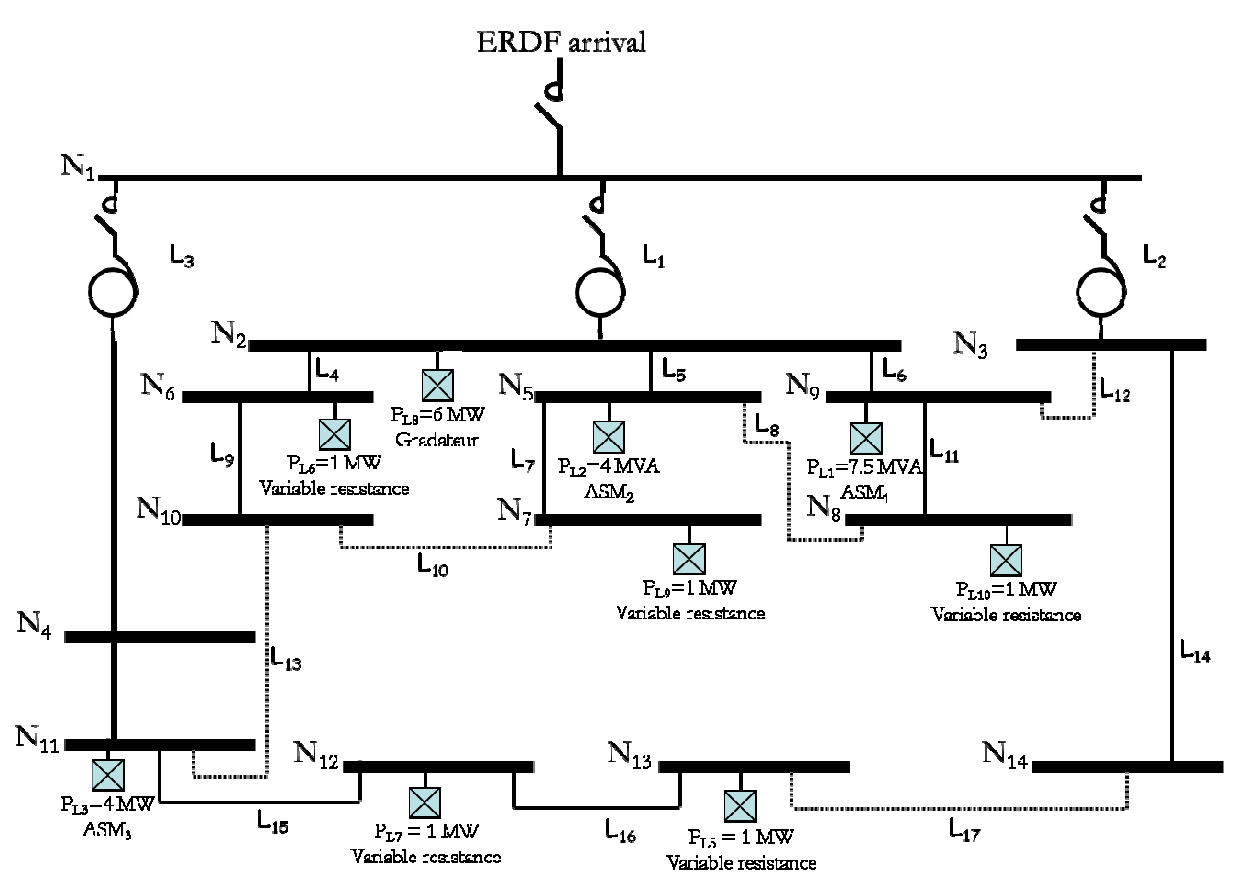
\includegraphics[width=1\textwidth]{NwImages/PREDIS}
	\captionof{figure}{The PREDIS/Urban Distribution Network}
	\labelFigure{fig:predisnw}
    \end{minipage}
    \begin{minipage}[h]{.35\textwidth }
    \centering
	\begin{tabular}{cc}
	\hline
	Voltage & $11$ kV\\
	% \hline
	\rowcolor{gray!15}
	Power & $100$ MVA\\
	% \hline
	Current &  $5248.6$ A\\
	% \hline
	\rowcolor{gray!15}
	Impedance & $1.21$ $\Omega$\\
	\hline
	\end{tabular}
	\caption{PREDIS - Base Values}
	\labelTable{predisbase}

	\vspace*{1 cm}

	\begin{tabular}{cc}
	% \hline
	\rowcolor{gray!25}
	\textbf{Lines} & \textbf{I max}\\
	\hline
	$7$, $8$, $10$ \& $11$ & $195$ A\\
	% \hline
	\rowcolor{gray!15}
	$14$ & $302$ A\\
	% \hline
	$4$, $9$ \& $15-17$ & $363$ A\\
	% \hline
	\rowcolor{gray!15}
	$6$ & $402$ A\\
	% \hline
	$5$ & $538$ A\\
	% \hline
	\rowcolor{gray!15}
	$1-3$, $12$ \& $13$ & $1$ pu\\
	\hline
	\end{tabular}
	\caption{PREDIS - $I_{max}$}
	\labelTable{predisImax}
    \end{minipage}%
\end{table}


\begin{table}[!h]
    \begin{minipage}[!h]{.5\textwidth}
	\centering
	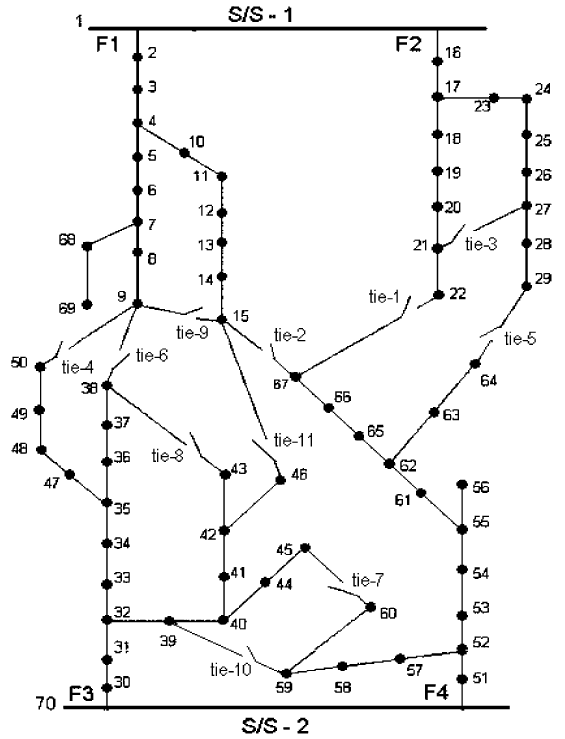
\includegraphics[width=0.8\textwidth]{NwImages/Rural_Network}
	\captionof{figure}{The Rural Distribution Network}
	\labelFigure{fig:dasnw}
    \end{minipage}
    \begin{minipage}[h]{.5\textwidth }
    \centering
	\begin{tabular}{cc}
	\hline
	Voltage & $11$ kV\\
	% \hline
	\rowcolor{gray!15}
	Power & $10$ MVA\\
	% \hline
	Current &  $524.86$ A\\
	% \hline
	\rowcolor{gray!15}
	Impedance & $12.1$ $\Omega$\\
	\hline
	\end{tabular}
	\caption{Rural Network - Base Values}
	\labelTable{dasbase}

	\vspace*{1 cm}

	\begin{tabular}{cc}
	% \hline
	\rowcolor{gray!25}
	\textbf{Lines} & \textbf{I max}\\
	\hline
	Tie Lines & $234$ A\\
	% \hline
	\rowcolor{gray!15}
	$1-18$, $17-23$ & $270$ A\\
	$31-39$, $52-57$ & $270$ A \\
	% \hline
	\rowcolor{gray!15}
	$9-16$, $24-30$ & $208$ A\\
	$40-51$, $58-68$ & $208$ A\\
	\hline
	\end{tabular}
	\caption{Rural Network - $I_{max}$}
	\labelTable{dasImax}
    \end{minipage}%
\end{table}

The two networks are varied in nature, and they were chosen with this very thought in mind. The urban network is smaller in size, with $14$ buses and $17$ lines. The rural network has $69$ buses and $79$ lines. The application of the developed algorithm to two different networks should ideally yield different results, and it would be interesting to compare and contrast them with one another.\\

The PREDIS network already has DRES connected. However, the rural network has no DRES data. Therefore, using a program developed by Marie-C\'{e}cile Alvarez-Herault\footnote{Marie-C\'{e}cile Alvarez-Herault is an associate professor at Grenoble INP, and a researcher at G2E Lab, where she works in the SYREL Team.}, DRES were randomly connected to the network for a $30\%$ insertion rate.\\

A load flow on the networks (using the applied models developed in \refSectionOnly{sec:appliedmodels}) showed that the problems associated with the two networks were indeed as thought. The urban network had many violations of current and voltage limits, while the rural network had fewer of the same.

\section {Models Applied to Test Networks}
\labelSection{sec:appliedmodels}

\lettrine[nindent=0pt]{T}{wo} load curves were created for each of the networks, based on the models explained earlier. The first one (model A) involved a simple association of one load type to each node in the networks.\\

In the second model (model B), for each node in both the test networks, a pseudo-random percentage of each of the load types was assigned. The assignment was pseudo-random in the sense that care was taken to see that the percentage of certain load types (for e.g.\ lighting) did not become unnaturally high. Typically, the load types were randomly assigned a percentage in the ranges shown in \refTableOnly{RICLperc}.\\

\begin{table}[H]
\centering
\begin{tabular}{ccc}
% \hline
\rowcolor{gray!25}
\textbf{Load Type} & \textbf{PREDIS Network} & \textbf{Rural Network}\\
\hline
Residential & $5-80$\% & $8-50$\% \\
% \hline
\rowcolor{gray!15}
Industrial & $5-50$\% & $20-75$\% \\
% \hline
Commercial & $0-50$\% & $5-70$\% \\
% \hline
\rowcolor{gray!15}
Lighting & $5-15$\% & $5-15$\% \\
\hline
\end{tabular}
\caption{Load Percentages}
\labelTable{RICLperc}
\end{table}

Based on these percentages, the two models were adapted to the two networks, and the day-ahead load curves were derived. The curves for both models are shown in \refFigureOnly{fig:dayaheadloadcurves}.\\

\begin{figure}[!h]
\begin{minipage}[!h]{.5\textwidth}
	\centering
    \setlength\figureheight{5cm}
    \setlength\figurewidth{6cm}
	% This file was created by matlab2tikz v0.4.6 running on MATLAB 8.2.
% Copyright (c) 2008--2014, Nico Schlömer <nico.schloemer@gmail.com>
% All rights reserved.
% Minimal pgfplots version: 1.3
% 
% The latest updates can be retrieved from
%   http://www.mathworks.com/matlabcentral/fileexchange/22022-matlab2tikz
% where you can also make suggestions and rate matlab2tikz.
% 
\begin{tikzpicture}

\begin{axis}[%
width=\figurewidth,
height=\figureheight,
scale only axis,
xmin=1,
xmax=24,
xtick={ 0,  4,  8, 12, 16, 20, 24},
xlabel={Time (hour)},
ymin=8,
ymax=28,
ytick={8, 12, 16, 20, 24, 28},
ylabel={Demand (MW)},
axis x line*=bottom,
axis y line*=left,
legend style={draw=black,fill=white,legend cell align=left, at={(0.5,-0.25)},anchor=north, legend columns=1}
]
\addplot [color=red,solid,mark=asterisk,mark options={solid}]
  table[row sep=crcr]{
0	13.075	\\
1	12.425	\\
2	11.2375	\\
3	11.5375	\\
4	10.6	\\
5	10.3	\\
6	11.475	\\
7	11.4625	\\
8	19.0625	\\
9	23.875	\\
10	24.6125	\\
11	24.9625	\\
12	25.5	\\
13	23.2875	\\
14	24.675	\\
15	24.475	\\
16	24.425	\\
17	23.7875	\\
18	23.325	\\
19	22.3125	\\
20	19.1375	\\
21	17.9625	\\
22	16.15	\\
23	15.5	\\
};
\addlegendentry{PREDIS Network - Model A};

\addplot [color=blue,solid,mark=+,mark options={solid}]
  table[row sep=crcr]{
0	18.496225	\\
1	17.036725	\\
2	15.260025	\\
3	16.0541	\\
4	15.161975	\\
5	14.386975	\\
6	14.802225	\\
7	13.498	\\
8	15.3973125	\\
9	17.417625	\\
10	18.01275	\\
11	18.69725	\\
12	18.995375	\\
13	17.869	\\
14	19.264625	\\
15	18.967625	\\
16	19.058125	\\
17	18.8933125	\\
18	23.422125	\\
19	24.88935	\\
20	24.3281	\\
21	23.91285	\\
22	23.380475	\\
23	21.920975	\\
};
\addlegendentry{PREDIS Network - Model B};

\end{axis}
\end{tikzpicture}%
\end{minipage}
\begin{minipage}[!h]{.5\textwidth}
	\centering
	\setlength\figureheight{5cm}
    \setlength\figurewidth{6cm}
	% This file was created by matlab2tikz v0.4.6 running on MATLAB 8.2.
% Copyright (c) 2008--2014, Nico Schlömer <nico.schloemer@gmail.com>
% All rights reserved.
% Minimal pgfplots version: 1.3
% 
% The latest updates can be retrieved from
%   http://www.mathworks.com/matlabcentral/fileexchange/22022-matlab2tikz
% where you can also make suggestions and rate matlab2tikz.
% 
\begin{tikzpicture}

\begin{axis}[%
width=\figurewidth,
height=\figureheight,
scale only axis,
xmin=1,
xmax=24,
xtick={ 0,  4,  8, 12, 16, 20, 24},
xlabel={Time (hour)},
ymin=1,
ymax=4,
ylabel={Demand (MW)},
axis x line*=bottom,
axis y line*=left,
legend style={draw=black,fill=white,legend cell align=left, at={(0.5,-0.25)},anchor=north, legend columns=1}
]

\addplot [color=red,solid,mark=triangle,mark options={solid}]
  table[row sep=crcr]{
0	2.349405	\\
1	2.20301	\\
2	2.042415	\\
3	1.99943	\\
4	1.99943	\\
5	1.95381	\\
6	2.00256	\\
7	2.59775	\\
8	1.699105	\\
9	1.8097	\\
10	2.518825	\\
11	2.59002	\\
12	2.384425	\\
13	2.64015	\\
14	2.469825	\\
15	1.85725	\\
16	2.234675	\\
17	2.170975	\\
18	3.533	\\
19	3.68714	\\
20	3.785935	\\
21	3.54921	\\
22	3.187735	\\
23	2.725685	\\
};
\addlegendentry{Rural Network - Model A};

\addplot [color=blue,solid,mark=square,mark options={solid}]
  table[row sep=crcr]{
0	2.05807563	\\
1	1.7963816	\\
2	1.57114753	\\
3	1.51164628	\\
4	1.51164628	\\
5	1.42596326	\\
6	1.47316896	\\
7	2.22160334	\\
8	1.91887959	\\
9	2.25947876	\\
10	2.86462259	\\
11	2.87541732	\\
12	2.67237475	\\
13	2.8661525	\\
14	2.84984517	\\
15	2.2010163	\\
16	2.69893055	\\
17	2.56839365	\\
18	3.556118	\\
19	3.66603836	\\
20	3.80485395	\\
21	3.65398318	\\
22	3.28427879	\\
23	2.68812165	\\
};
\addlegendentry{Rural Network - Model B};

\end{axis}
\end{tikzpicture}%
\end{minipage}
\caption{Day-ahead Load Curves (Models A \& B) for the Test Networks}
\labelFigure{fig:dayaheadloadcurves}
\end{figure}

As for the DRES production, the cumulative values are shown in \refFigureOnly{fig:dayaheadDREScurves}.\\

\begin{figure}[!h]
\begin{minipage}[!h]{.5\textwidth}
	\centering
    \setlength\figureheight{5cm}
    \setlength\figurewidth{6cm}
	% This file was created by matlab2tikz v0.4.6 running on MATLAB 8.2.
% Copyright (c) 2008--2014, Nico Schlömer <nico.schloemer@gmail.com>
% All rights reserved.
% Minimal pgfplots version: 1.3
% 
% The latest updates can be retrieved from
%   http://www.mathworks.com/matlabcentral/fileexchange/22022-matlab2tikz
% where you can also make suggestions and rate matlab2tikz.
% 
\begin{tikzpicture}

\begin{axis}[%
width=\figurewidth,
height=\figureheight,
scale only axis,
xmin=1,
xmax=24,
xlabel={Time (hour)},
ymin=0,
ymax=16,
ylabel={Production (MW)},
axis x line*=bottom,
axis y line*=left,
legend style={draw=black,fill=white,legend cell align=left, at={(0.5,-0.25)},anchor=north, legend columns=1}
]
\addplot [color=blue,solid]
  table[row sep=crcr]{
0	3.852	\\
1	5.728	\\
2	5.338	\\
3	4.864	\\
4	1.707	\\
5	2.045	\\
6	1.749	\\
7	0.532	\\
8	1.006	\\
9	8.0293793	\\
10	7.3152759	\\
11	11.8102414	\\
12	15.528	\\
13	9.4014483	\\
14	13.7370345	\\
15	10.3953103	\\
16	5.206	\\
17	1.792	\\
18	7.956	\\
19	3.652	\\
20	3.417	\\
21	6.016	\\
22	0.514	\\
23	8.088	\\
};
\addlegendentry{PREDIS Network};

\end{axis}
\end{tikzpicture}%
\end{minipage}
\begin{minipage}[!h]{.5\textwidth}
	\centering
	\setlength\figureheight{5cm}
    \setlength\figurewidth{6cm}
	% This file was created by matlab2tikz v0.4.6 running on MATLAB 8.2.
% Copyright (c) 2008--2014, Nico Schlömer <nico.schloemer@gmail.com>
% All rights reserved.
% Minimal pgfplots version: 1.3
% 
% The latest updates can be retrieved from
%   http://www.mathworks.com/matlabcentral/fileexchange/22022-matlab2tikz
% where you can also make suggestions and rate matlab2tikz.
% 
\begin{tikzpicture}

\begin{axis}[%
width=\figurewidth,
height=\figureheight,
scale only axis,
xmin=1,
xmax=24,
xlabel={Time (hour)},
ymin=0.8,
ymax=2,
ylabel={Production (MW)},
axis x line*=bottom,
axis y line*=left,
legend style={draw=black,fill=white,legend cell align=left, at={(0.5,-0.25)},anchor=north, legend columns=1}
]
\addplot [color=red,solid]
  table[row sep=crcr]{
0	1.3204366	\\
1	1.58013391	\\
2	1.67322503	\\
3	1.99318176	\\
4	1.4954867	\\
5	1.66521042	\\
6	1.43650239	\\
7	1.62284984	\\
8	1.60521016	\\
9	1.68773886	\\
10	1.51032673	\\
11	0.90721418	\\
12	1.61214652	\\
13	1.8977162	\\
14	1.95117643	\\
15	1.5312021	\\
16	1.76392663	\\
17	1.5445812	\\
18	1.98685491	\\
19	1.80166541	\\
20	1.5223008	\\
21	1.59099695	\\
22	1.76961399	\\
23	1.44837906	\\
};
\addlegendentry{Rural Network};

\end{axis}
\end{tikzpicture}%
\end{minipage}
\caption{Cumulative Day-ahead DRES Production Curves for the Test Networks}
\labelFigure{fig:dayaheadDREScurves}
\end{figure}

The curves show a major share of power coming from solar energy in the PREDIS network (understandably, given that it is an urban network) and a major share for wind power in the rural network (evident with a dip during midday, something that would have normally not happened with solar power). These are the models that have been utilized for the algorithm.\\

For the two networks, the maximum insertion rate of DRES is shown below. The values change every hour for both the networks.

\begin{table}[h]
\centering
\begin{tabular}{ccc}
% \hline
\rowcolor{gray!25}
& \textbf{Load Model A} & \textbf{Load Model B}\\
\hline
PREDIS Network & $60.89$\% (Hour $12$) & $81.75$\% (Hour $12$) \\
% \hline
\rowcolor{gray!15}
Rural Network & $99.69$\% (Hour $3$) & $131.86$\% (Hour $3$) \\
\hline
\end{tabular}
\caption{DRES Insertion Rates}
\labelTable{dresins}
\end{table}

In the case where the insertion rate is higher than $100$\%, there is a possibility for injection of power from the distribution network to the transmission network. This is unadvisable and causes other constraints, which will be treated in due course of development.



% SVN info for this file
%!TEX root = report.tex

\svnidlong
{$HeadURL$}
{$LastChangedDate$}
{$LastChangedRevision$}
{$LastChangedBy$}

\chapter{The Algorithm}
\labelChapter{algo}

\begin{introduction}
This chapter describes the multi-temporal day-ahead optimization algorithm for distribution networks, its various components, and also provides some insights into various development examples.
\end{introduction}


\section{Definition of Requirements}

\lettrine[nindent=-0pt]{T}{he} algorithm developed makes use of the results of forecasting of DRES and loads in a particular distribution network to provide a day-ahead schedule for that distribution network. Two main requirements were laid down in the beginning:\\

\begin{itemize}
\item The algorithm has to be multi-objective, making use of a combination several methods to achieve optimization.\\
\item The algorithm has to be modular in nature, so that other methods of optimization can be added, or the current methods modified, in future. This will also permit the addition of results from state estimation in unobservable or partially observable distribution networks.\\
\item The algorithm has to be user-friendly, providing outputs that an end-user can understand.
\end{itemize}

\section{Initial Development Ideas}
\lettrine[nindent=0pt]{B}{efore} developing the actual algorithm, a lot of initial ideas were developed and tested with respect to individual components in the algorithm. Some of the components, the successful development of which later led to the development of the  algorithm are elucidated below.\\

Right from the beginning, reconfiguration was envisaged to be one of the major components. As explained in \refChapterOnly{stateofart}, most of the current literature considers only a snapshot of the network conditions for reconfiguration. However, in real networks, conditions often change. This means that the reconfiguration performed once should continue to be the optimal for every condition that succeeds the condition for which it was performed. One solution for this problem could be to reconfigure every time the conditions in the network change. But since reconfiguration in distribution networks is a cumbersome, often expensive task, it is good that it is not done in that manner. Therefore, another solution which can maintain optimality without requiring frequent reconfigurations has to be chosen.\\

In order to find such a solution, means to decrease the number of reconfigurations were investigated. A simple reconfiguration function based on the well known Merlin and Back method was tested on two different networks with various inputs. As will be seen in \refChapterOnly{results}, one of the methods that made use of the maximum values of loads and DRES production for the entire time horizon under consideration performed consistently well, with results very close to that of hourly reconfiguration. This was also tested with the final reconfiguration algorithm, and with this working well, was implemented in the final solution. Once it was proven that the number of reconfigurations could potentially be reduced by using maximum values of load and DRES parameters, development of other optimization methods was undertaken.\\

The development of these methods was fairly simple too. Initially, only voltage violations were taken into account, with current violations being added later. For reactive power setting (VVC) of generators, a \textsc{matlab} function - \emph{fmincon} with objectives to eliminate the voltage violations was used. Each DRES has reactive power limits, which is a function of the active power it produces. These limits formed the upper and lower bounds for the optimization, while the objective function was the cumulative difference between the voltages of the affected nodes and an arbitrarily chosen constant which was within the acceptable voltage limits ($0.95\ \mathrm{pu} < V < 1.05\ \mathrm{pu}$). The input to the function `$x0$' started at a value of zero, which implied that the generators were generating only active power. \emph{fmincon} sets the reactive powers of these generators. Initially, irrespective of the location of the violations, all the generators were involved in this process. This was changed later with a selection routine, based on the type and location of the violation.\\

Load Reduction was developed using \emph{fmincon} as well. For simplicity, it was assumed that an arbitrary percentage of load could be reduced at arbitrarily chosen nodes in a given distribution network, if the need arose. The upper and lower bounds were the actual load on the node, and the reduced load (based on the arbitrarily chosen percentage) respectively. The objective function for load reduction is the same as the one used in VVC.\\

OLTC control was among the easiest to implement. The OLTCs to be operated were decided based on the localisation of violations to their respective feeders, each of which might or might not be serviced by OLTCs. In the \emph{fmincon} optimization for the OLTC setting, the input `$x0$' had to be modified during every iteration to the nearest OLTC setting available. The upper and lower bounds were the two extreme settings of the respective OTLCs. The only difference with using the OLTCs was that once any tap change was made, it would not automatically change the next hour (unlike DRES active power, or loads). Therefore, the input to the optimisation done next hour had to take into account the old positions of the tap.\\

With the merging of the three different methods into one optimisation, taking into account the respective constraints for each of the variables, a modular function was made and tested. All the three methods have costs associated to them. However, since their sole purpose is to get rid of violations, it was initially decided to not favour one method over another. This means that the objective of the \emph{fmincon} will be to solely use any method, or a combination of these methods, to rid the network of violations.\\

In future, the \emph{fmincon} function can be replaced with a multi-objective function that minimizes the cost while getting rid of violations. This will make the cost of each of the method very important as it can have a major effect on which methods are chosen.\\

The addition of current violations required a few changes to be made in the functions. Management of voltage violations was still implemented with nearby nodes only. But load reduction and VVC had to be activated for all the nodes downstream of the line with overcurrent. Also, since \emph{fmincon} cannot perform multi-objective optimization, three separate optimization routines had to be created, two for current and voltage violations each, and one for both violations (when they occur together). With all the individual components working, further development could be made.

\section{Components and Functions of the Final Algorithm}
\labelSection{algo:components}

\lettrine[nindent=-0pt]{T}{he} various components of the final algorithm, which make use of the functions developed initially are listed below, with a brief description about each of the components following it. The next section will elaborate on the use of these components, and thus complete the idea.

\begin{figure}[!h]
% A component diagram will have to be included here.
\pgfdeclarelayer{background}
\pgfdeclarelayer{foreground}
\pgfsetlayers{background,main,foreground}

\tikzstyle{lcomp}=[draw, fill=blue!20, text width=5em, 
    text centered, minimum height=2.5em,text centered]

\tikzstyle{ann} = [above, text width=5em]

\tikzstyle{program} = [lcomp, text width=6em, fill=red!20, 
    minimum height=6em, minimum width=10em, rounded corners,text centered, drop shadow]

\tikzstyle{global} = [lcomp, text width=6em,
    fill=green!20, minimum height=6em, minimum width=8em, rounded corners,text centered, drop shadow]

\tikzstyle{reconf} = [lcomp, text width=8em, fill=gray!10, 
    minimum height=4em, minimum width=8em, rounded corners,text centered, drop shadow]

\tikzstyle{lf} = [lcomp, text width=8em, fill=yellow!20, 
    minimum height=4em, minimum width=8em, rounded corners,text centered, drop shadow]

\tikzstyle{local} = [draw, circle, text width=3em, fill=blue!20,
	minimum height=3em, minimum width=3em, text centered, circular drop shadow]

\tikzstyle{blank} = [node distance=1cm,minimum width=-1cm]

\tikzstyle{vecArrow} = [thick, decoration={markings,mark=at position 0 with {\arrowreversed[semithick]{open triangle 60}},mark=at position
   1 with {\arrow[semithick]{open triangle 60}}},
   double distance=1.4pt, shorten >= 5.5pt, shorten <= -5.5pt,
   preaction = {decorate},
   postaction = {draw,line width=1.4pt, white,shorten >= 4.5pt, shorten <= 4.5pt}]
\tikzstyle{innerWhite} = [semithick, white,line width=1.4pt, shorten >= 4.5pt, shorten <= -7pt]

\centering
\begin{tikzpicture}
	% Main Program
    \node [program] (prog) {Main Program};

    % Reconfiguration
    \node [blank,right of=prog, node distance=1cm] (b1) {};
    \node [reconf,below of=prog, node distance=3.5cm] (rec) {Reconfiguration Algorithm};
    \node [reconf, right of=rec,node distance=5cm] (recdb) {Reconfiguration Database};
    \node [blank, left of=rec, node distance=2cm] (b5) {};

    % Load Flow
    \node [lf, above of=prog, node distance=3cm] (ld) {Load Flow};

    % Local Management
    \node [blank, below of=prog, node distance=3cm] (b2) {};
    \node [local, left of=prog, node distance=4cm] (lr) {LR};
    \node [local, left of=lr, node distance=2cm] (vvc) {VVC};
    \node [blank, left of=lr, node distance=1cm] (b3) {};
    \node [blank, right of=lr, node distance=1cm] (b4) {};
    \node [local, below of=b3, node distance=1.5cm] (oltc) {OLTC};
    \node [blank, above of=oltc, node distance=3cm] (lmg) {\large Local Management};

    % Global Management
    \node [global,right of=prog, node distance=5cm] (gm) {Global Management};

    \begin{pgfonlayer}{background}
        \path (vvc.west)+(-0.5,1.8) node (a) {};
        \path (oltc.south -| lr.east)+(+0.5,-0.2) node (b) {};
        \path[fill=blue!10,rounded corners, draw=black!50, dashed]
            (a) rectangle (b);

        \path (rec.north west)+(-0.5,0.5) node (c) {};
        \path (recdb.south east)+(+0.5,-0.5) node (d) {};
        \path[fill=gray!05,rounded corners, draw=black!50, dashed]
            (c) rectangle (d);
    \end{pgfonlayer}

    \draw[vecArrow] (prog.north)+(0,0.4) to (ld);
    \draw[innerWhite] (prog.north)+(0,0.4) to (ld);

    \draw[vecArrow] (lmg.north)+(0,0.4) |- (ld);
    \draw[innerWhite] (lmg.north)+(0,0.4) |- (ld);

    \draw[vecArrow] (gm.north)+(0,0.4) |- (ld);
    \draw[innerWhite] (gm.north)+(0,0.4) |- (ld);

	\draw[vecArrow] (b4)+(0.65,0) to (prog);
    \draw[innerWhite] (b4)+(0.65,0) to (prog);

    \draw[vecArrow] (prog.east)+(0.4,0) to (gm);
    \draw[innerWhite] (prog.east)+(0.4,0) to (gm);

	\draw[vecArrow] (rec.north)+(0,0.9) to (prog.south);
    \draw[innerWhite] (rec.north)+(0,0.9) to (prog.south);

    \draw[vecArrow] (recdb.north)+(0,0.9) to (gm.south);
    \draw[innerWhite] (recdb.north)+(0,0.9) to (gm.south);

    \draw[vecArrow] (gm.east)+(0.45,0) to node {} +(1.2,0) to node {} +(1.2,-5.3) to node {} +(-11.5,-5.3) to node {} +(-11.5,-2.45);
    \draw[innerWhite] (gm.east)+(0.45,0) to node {} +(1.2,0) to node {} +(1.2,-5.3) to node {} +(-11.5,-5.3) to node {} +(-11.5,-2.45);
    
\end{tikzpicture}
\caption{Components of the Algorithm}
\labelFigure{fig:algocomp}
\end{figure}

\subsection{Reconfiguration Component}

The reconfiguration component is a modular function that provides different reconfigured states for radially operated networks based on the load and DRES conditions in it. At the heart of the function is a modified version of the fuzzy multi-objective routine developed in \cite{Das2006}. Although there is more recent literature available, the reason why a simpler and older algorithm was chosen initially with an intention to have a perfect working example. Owing to the modular nature of the algorithm presented here, all one has to do to change the reconfiguration component is to write another routine with any reconfiguration method one wishes to have, and replace the existing one with the new one.\\

The current routine uses a branch exchange method to reconfigure networks. First, all the normally open lines are pre-selected as possible candidates for exchange. A reduction step calculates the voltage difference between the nodes on either end of the candidate lines and chooses only the lines where it is higher than a pre-set value $\epsilon$. This speeds up the process as the closing of lines with very close terminal potentials will not have a major effect on network conditions. However, it is to be kept in mind that a very high value of $\epsilon$ will deem even suitable exchange processes unfit and cause the reconfiguration to fail. Typically, $\epsilon=0.01pu$. The line with the highest voltage difference across it is chosen as the line to be exchanged. This process can seem cumbersome, but it will help when other, more complex selection criteria are developed in future. If there are no lines across which the voltage difference is higher than $\epsilon$, the routine terminates.\\

If a line is selected, it is closed and forms a loop. Then, each line in the loop is opened, restoring radiality, and the state of the distribution network is ascertained. The routine checks four objectives for every line opened, namely the reduction in power losses, the deviation in node voltages, deviation in line currents, and deviation in feeder currents. Each of these is assigned a membership function, as explained in \refAppendixOnly{algoappendix}, with values between 0 and 1, based on how they perform.\\

For each line, the minimum value from each of these membership functions is chosen. Then, when all the lines have been opened one by one and their associated minimum membership function values noted, the maximum of these minimum membership functions is calculated, and the line associated with this value is chosen as the line to be exchanged. This opened line is not pre-selected later as a potential candidate. In the next iteration, once again, the pre-selection and selection processes happen, and this goes on and on until there are no lines left to be exchanged. Thus, reconfiguration is achieved.

\subsection{Local Management Component}
The local management component is used to manage violations locally. Making use of the different optimization routines developed earlier, the local management function can effectively manage the violations that are deemed ``local'' by the algorithm. How the algorithm deems violations ``local'' or otherwise is explained later. In a way, the local management component integrates all the optimization options except for reconfiguration.\\

Firstly, when invoked, the function determines the type, and number of violations. For the nodes where the violations have occurred, the function then decides which nodes to use for the different optimization methods available. It does this by first finding the nodes which can potentially be used for optimization, and then filters the unwanted nodes out by finding which nodes actually have the required resources to perform optimization. For example, nodes immediately surrounding a node with violations are available for VVC. But among these nodes, the ones without any DRES connected are filtered out. Nodes for load reduction are also chosen only where such an option is available. The function then groups all the values of initial inputs into one variable $x0$, which is then sent to different \emph{fmincon} functions depending on the types, as already explained in the previous section.\\

The variable $x0$ is de-constructed inside the respective \emph{fmincon} function. This is done with the use of a lookup table for cases. Depending upon the location and type of violations in a network, not all the optimization methods may be available. In order to easily pass information to the optimization function about what methods are available and to facilitate easy deconstruction of $x0$, the case is determined from a lookup table (\refTableOnly{caselocal}).

\begin{table}[!h]
\centering
\begin{tabular}{cccc}
% \hline
\rowcolor{gray!25}
\textbf{OLTC} & \textbf{LR/LS} & \textbf{VVC} & \textbf{Case}\\
\hline
$0$ & $0$ & $0$ & $1$\\
\rowcolor{gray!15}
$0$ & $0$ & $1$ & $2$\\
$0$ & $1$ & $0$ & $3$\\
\rowcolor{gray!15}
$0$ & $1$ & $1$ & $4$\\
$1$ & $0$ & $0$ & $5$\\
\rowcolor{gray!15}
$1$ & $0$ & $1$ & $6$\\
$1$ & $1$ & $0$ & $7$\\
\rowcolor{gray!15}
$1$ & $1$ & $1$ & $8$\\
\hline
\end{tabular}
\caption{Case Selection based on Available Optimization Methods}
\labelTable{caselocal}
\end{table}

Obviously, if the case is $1$, the local management function stops, as there is no optimization to be carried out. Otherwise, the program sends $x0$ and other variables to the respective optimization functions (depending on the type of violations).\\

The result is then analysed to see if the number of violations are reduced or not. If no, then local management for the violations in question is deemed useless. The cost for managing violations is also checked, and if it is more than the cost that would be incurred if the violations were left as is, then the local management is deemed useless as well.\\

The most important thing about the local management function is that it optimizes the network only for the hour during the day for which it is launched.

\subsection{Global Management Component}
If there are violations in the network are deemed to be ``global'' rather than ``local'', the global management function is invoked. This function is a recursive umbrella function which makes use of all the developed optimization options. The function, once launched, creates a parallel environment from that of the main program that launches it. It then proceeds to analyse, on two separate paths, different solutions for optimization during the rest of the day.\\

Basically, what the function does is that from the hour \emph{h} when it is launched, it splits the scheduling horizon into two. The first horizon uses reconfiguration for hour \emph{h} and also uses the \emph{local optimization} methods in a global context, and then for the remaining time in the day, continues to function as if the main program would. The second horizon doesn't use reconfiguration, and tries to absolve the network of violations using all the \emph{local management} methods, in the global context. Then, it proceeds to work like the main program, for the remaining time in the day. So technically speaking, for the remaining time in the day, if there are more violations that are ``global'' in nature, the same function is launched recursively. For each and every recursion in both the scheduling horizons, the costs are calculated, and at the end of that recursion, the costs are compared. The solution with the least cost is chosen as the solution to be fed back to the calling function. The global management component is an exhaustive search component whose search horizon becomes narrower as time progresses.

\subsection{Other Components and Functions}
Several other functions have been developed to be used by (one of) the component(s). They have all been written as separate functions, and each of these functions is described below.\\

A loop finding function has been developed to be used by the reconfiguration component, in order to find the loops created by closing NO switches. It achieves this by finding the shortest paths from nodes on either side of the NO line to the substation, with care taken to see that the paths do not go through the line itself. The function uses Dijkstra's algorithm to find the shortest paths, considering the network as a graph with all edges possessing the same weight. In any case, a radial network with only one NO closed, forming one loop, will only have two paths to the substation from a node in the loop.\\

A function to remove sub-station nodes from nodes identified for VVC is implemented too. Since nodes are selected through linear search in an iterative manner, the input of a sub-station node to an iteration will result in the selection of nodes that are on other branches of the network, and hence after every iteration, this function is called to remove the sub-station nodes.\\

A load flow function, originally developed by Marie-C\'{e}cile Alvarez-Herault, is integral to the functioning of the algorithm. At almost every step imaginable, a load flow is done to assess the network state. This provides us with the bus voltages and line currents, two of the most important parameters in the network.\\

The three \emph{fmincon} functions, labelled `\emph{onlyV}', `\emph{onlyI}' and `\emph{bothVI}' are used to treat different violation occurrences separately. Given that the optimization has only one objective, the treatment of both current and voltage violations involves making a single objective for both the constraints. This is not really easy, and in future, it has been envisaged that this will be replaced with a multi-objective optimization function. Finally, another function which identifies the sub-station node for OLTC action is also developed.

\section{Association of Costs}

\lettrine[nindent=0pt]{T}{he} association of costs to all the constraints is a very important step in the algorithm. It has the potential to influence the results greatly, and a wrong choice of costs can provide unusable results. With this in mind, one cannot stress enough, the importance of an economic model for all the constraints.\\

In any case, if the models are so developed that they are complete and take into account, all the issues that might arise out of actions for optimization, a solution with the lowest global cost can be obtained. This means that while the solution may cause a reduction in the lifetime of certain expensive devices, implementing the solution and replacing these devices once they fail will still be a cheaper solution than implementing other solutions. However, the development of such a model is cumbersome and will have to be left for the future.\\

In this thesis, the possibility of development of a simplified  model is discussed and the choice of actual costs for constraints is shown.

\subsection{Economic Model for Switching}
As understood earlier, reconfiguration cannot be done often, the reason for this being either the logistical difficulty in doing so, or the danger of reduced lifetime of switches. A high cost associated to switching can deter the algorithm from reconfiguring at will, but might not provide us with the optimal configuration with the lowest global cost. A simple model for cost of switching can be described as:

\begin{align*} 
Cost/switching&=\frac{C_{sw}}{n_{sw}}+ C_{OM}+C_{log}\\
C_{OM}&=c*f(t_{sw})
\end{align*}\\

Where $C_{sw}$ is the cost of purchasing the switch, $n_{sw}$ is the number of switching operations the switch is rated for during its entire lifetime, $C_{OM}$ is the estimated operation and maintenance costs of the switch during the time between switching operations (which takes into account the extra maintenance required for frequent switching and is therefore a constant value times a function of the interval between switching operations), and $C_{log}$ is the cost of logistics.

\subsection{Economic Model for Load Reduction/Shedding}
Economic models for load reduction/shedding are already present today and are used by aggregators and other such actors in the distribution network. Their model essentially provides them with the profits they have to make in order to survive. While some may argue that clients of aggregators are often short changed, it is noteworthy that the models they have developed are the most efficient, because their survival literally hinges on its infallibility.

\subsection{Economic Model for OLTC}
Like switches in the network, OLTCs can also not be operated frequently. And since their action is also a kind of switching, the model used for switching can be adapted for OLTCs as well.

\begin{align*} 
Cost/operation&=\frac{C_{OLTC}}{n_{op}}+ C_{OM}+C_{log}\\
C_{OM}&=c*f(t_{op})
\end{align*}\\
Where $C_{OLTC}$ is the cost of purchasing the OLTC, $n_{op}$ is the number of operations the OLTC is rated for during its entire lifetime, $C_{OM}$ is the estimated operation and maintenance costs of the OLTC during the time between switching operations (which takes into account the extra maintenance required for frequent switching and is therefore a constant value times a function of the interval between operations), and $C_{log}$ is the cost of logistics.

\subsection{Economic Model for Voltage VAr Control}
Compensating distributed generators for their reactive power supply is fairly simple. Converters today are capable of active - reactive power conversion without any additional effort required. Therefore, the generators may be paid the same amount of money for the reactive power they produce as the active power they produce. Additionally, an annual contractual income may also be earned by the owners of these generators, for agreeing to participate in reactive power compensation.

\subsection{Economic Model for Violations}
Violations of voltage and current in networks are bad for several reasons. A lower-than-normal voltage or higher-than-normal current will accelerate the degradation of conductors, while higher voltages will cause degradation of insulation. The fact that the estimation of short and long-term effects of repeated occurrences of violations is difficult does not help either.\\

The development of an economic model for violations is however very important because it is based on this model that the algorithm will decide whether clearing specific violations is economically feasible or not. For an initial assumption, the cost of violations can be a linear, or non-linear function of the ageing it causes on lines or insulation. In future work, complete models can be made based on detailed calculations of the effects of violations on the network.

\section{Working of the Algorithm}
\lettrine[nindent=0pt]{B}{ased} on the components developed and described in the previous section, the working of the algorithm is described here, and illustrated in \refFigureOnly{fig:algoflch} in \refAppendixOnly{algoappendix}.\\

The main program first reads the data for the network to be optimized. This data is stored in a \emph{.mat} file in a particular format described in \refAppendixOnly{algoappendix}. Once this data is loaded, the program creates a database of reconfigurations. As explained earlier, this database contains a network configuration for every hour of the day for which forecast data is available, based on the maximum value of loads and DRES in each node for the remaining period of time in the day. This database will be made use of later.\\

The program then launches an iterative violation finder. Say at hour $t_0$, violations are found. The nature, and the location of these violations in the network are determined, in order to ascertain the type of violation. Then, they are classified as either \emph{local} or \emph{global}. In this case, this is determined by whether the violations are present in the same feeder or not, although other selection criteria may also be employed. If the violations are deemed to be \emph{local}, the program launches the \emph{local management} component, which does its job as explained previously. Otherwise, the \emph{global management} component is launched. The operation then proceeds as explained in \refSectionOnly{algo:components}, under the \emph{Global Management Component}.
% SVN info for this file
%!TEX root = report.tex

\svnidlong
{$HeadURL$}
{$LastChangedDate$}
{$LastChangedRevision$}
{$LastChangedBy$}

\chapter{Results}
\labelChapter{results}

\begin{introduction}
  This chapter presents the results obtained from the algorithm when applied on two different distribution networks. Results obtained during initial development are also shown.
\end{introduction}

\section{Initial Results - Development}

\lettrine[nindent=0pt]{I}{nitially}, during the course of development, several results were obtained, many of which altered the choices made during the course of further work. The results of the Merlin and Back algorithm for various number and types of reconfigurations are shown in \refFigureOnly{fig:mandb}. The losses over a 24 hour period for the original networks are shown. Then, the losses for the same period are shown, if the network is reconfigured every hour for optimality. The maximum and average values of load (model A) and DRES at each node for the entire period is then calculated, and with these as input conditions, one reconfiguration is performed at the beginning of the day. The losses in both the cases for both the networks are also shown.\\

\begin{figure}[!h]
\begin{minipage}[!h]{.5\textwidth}
	\centering
    \setlength\figureheight{5cm}
    \setlength\figurewidth{6cm}
	% This file was created by matlab2tikz v0.4.6 running on MATLAB 8.2.
% Copyright (c) 2008--2014, Nico Schlömer <nico.schloemer@gmail.com>
% All rights reserved.
% Minimal pgfplots version: 1.3
% 
% The latest updates can be retrieved from
%   http://www.mathworks.com/matlabcentral/fileexchange/22022-matlab2tikz
% where you can also make suggestions and rate matlab2tikz.
% 
\begin{tikzpicture}

\begin{axis}[%
width=\figurewidth,
height=\figureheight,
scale only axis,
xmin=0,
xmax=24,
xtick={ 0,  4,  8, 12, 16, 20, 24},
xminorticks=true,
xlabel={Time (hour)},
ymin=0,
ymax=1200,
ylabel={Losses (kW)},
axis x line*=bottom,
axis y line*=left,
legend style={draw=black,fill=white,legend cell align=left, at={(0.5,-0.25)},anchor=north, legend columns=2}
]
\addplot [color=black,solid,line width=1.0pt]
  table[row sep=crcr]{
0	187.470852708396	\\
1	208.073264002775	\\
2	369.453812970541	\\
3	189.718454522433	\\
4	115.418958958224	\\
5	99.2368118293202	\\
6	159.410349961767	\\
7	145.184867621662	\\
8	506.841683410891	\\
9	875.089613674351	\\
10	658.59429508712	\\
11	447.370112257461	\\
12	479.747476017529	\\
13	876.014308683698	\\
14	1025.66991298176	\\
15	793.638695196897	\\
16	522.557408059643	\\
17	731.118595681807	\\
18	188.51698229905	\\
19	375.813228594712	\\
20	452.72643282892	\\
21	132.665389276462	\\
22	458.467025766648	\\
23	545.317597799103	\\
};
\addlegendentry{Original};

\addplot [color=blue,solid,line width=1.0pt]
  table[row sep=crcr]{
0	37.0992700523806	\\
1	30.3620650854819	\\
2	66.2180509631016	\\
3	31.8947685828755	\\
4	30.2290766611202	\\
5	23.0552961419536	\\
6	31.2138404230611	\\
7	26.3484341197884	\\
8	58.0183843249205	\\
9	72.6055806268167	\\
10	114.916329089854	\\
11	137.033387593966	\\
12	236.448536160519	\\
13	163.995249077653	\\
14	422.50083042695	\\
15	237.512954802552	\\
16	74.0303685398846	\\
17	85.0306701981773	\\
18	52.1605535837466	\\
19	79.9883240029414	\\
20	76.2800858210899	\\
21	41.59866233307	\\
22	115.253688184083	\\
23	100.458255996627	\\
};
\addlegendentry{Hourly};

\addplot [color=green,solid,line width=1.0pt]
  table[row sep=crcr]{
0	49.9906360840574	\\
1	58.8871181717937	\\
2	112.07616576048	\\
3	57.2916830921991	\\
4	31.5132123372294	\\
5	25.5056433559525	\\
6	33.2242924258097	\\
7	26.3484341197884	\\
8	58.0620198247339	\\
9	78.2954718226647	\\
10	113.37557755238	\\
11	155.029956450251	\\
12	247.599698220103	\\
13	155.961956971143	\\
14	471.862125347108	\\
15	302.633446508699	\\
16	101.021227926196	\\
17	85.0306701981773	\\
18	67.7191842226782	\\
19	80.1910226861102	\\
20	76.127792687114	\\
21	60.3880584185895	\\
22	115.253688184083	\\
23	100.458255996627	\\
};
\addlegendentry{Max.};

\addplot [color=red,solid,line width=1.0pt]
  table[row sep=crcr]{
0	64.9398184700778	\\
1	42.8598475862435	\\
2	72.6741675204701	\\
3	38.6113857960654	\\
4	40.8545281369965	\\
5	31.3749970536403	\\
6	55.4639759621944	\\
7	38.3979835758413	\\
8	82.2519796794319	\\
9	96.4950188875768	\\
10	108.251613746782	\\
11	142.507497274888	\\
12	281.180085965371	\\
13	173.810111568062	\\
14	717.850282405204	\\
15	424.866794619111	\\
16	79.3950740225591	\\
17	123.329593935162	\\
18	51.0609103975129	\\
19	110.057762182345	\\
20	114.529191965013	\\
21	51.9788980904906	\\
22	208.364036157857	\\
23	151.286743793291	\\
};
\addlegendentry{Avg.};

\end{axis}
\end{tikzpicture}%
\end{minipage}
\begin{minipage}[!h]{.5\textwidth}
	\centering
	\setlength\figureheight{5cm}
    \setlength\figurewidth{6cm}
	% This file was created by matlab2tikz v0.4.6 running on MATLAB 8.2.
% Copyright (c) 2008--2014, Nico Schlömer <nico.schloemer@gmail.com>
% All rights reserved.
% Minimal pgfplots version: 1.3
% 
% The latest updates can be retrieved from
%   http://www.mathworks.com/matlabcentral/fileexchange/22022-matlab2tikz
% where you can also make suggestions and rate matlab2tikz.
% 
\begin{tikzpicture}

\begin{axis}[%
width=\figurewidth,
height=\figureheight,
scale only axis,
xmin=0,
xmax=24,
xtick={ 0,  4,  8, 12, 16, 20, 24},
xminorticks=true,
xlabel={Time (hour)},
ymin=10,
ymax=110,
ylabel={Losses (kW)},
axis x line*=bottom,
axis y line*=left,
legend style={draw=black,fill=white,legend cell align=left, at={(0.5,-0.25)},anchor=north, legend columns=2}
]
\addplot [color=black,solid,line width=1.0pt]
  table[row sep=crcr]{
0	36.0418933408924	\\
1	28.4382759081625	\\
2	26.1215707561308	\\
3	21.6061502667575	\\
4	24.3378452311177	\\
5	22.4855092514709	\\
6	23.0639450119174	\\
7	40.4945348436625	\\
8	14.1245722984627	\\
9	15.7413514465241	\\
10	36.0505152919788	\\
11	51.0115231011965	\\
12	29.4802184601339	\\
13	39.5355852743295	\\
14	29.7385119880372	\\
15	16.8690444893987	\\
16	25.7830091609484	\\
17	27.5769625406691	\\
18	87.9169828226134	\\
19	100.697324204575	\\
20	100.968451139209	\\
21	93.5993669897117	\\
22	59.0483117906493	\\
23	49.0753737355887	\\
};
\addlegendentry{Original};

\addplot [color=blue,solid,line width=1.0pt]
  table[row sep=crcr]{
0	29.8637103345656	\\
1	22.6373141949504	\\
2	19.7053601216957	\\
3	16.4116305583722	\\
4	19.9512907898475	\\
5	17.8499022501022	\\
6	19.0806292192391	\\
7	33.3403060085935	\\
8	10.5720864610383	\\
9	11.7742154093067	\\
10	28.7151303060595	\\
11	40.6460576985657	\\
12	24.2471780796827	\\
13	28.0464514021789	\\
14	23.6915321890768	\\
15	13.4226343066141	\\
16	19.3640127836298	\\
17	19.1918976858241	\\
18	66.8954526444188	\\
19	76.5895757427226	\\
20	84.05212486573	\\
21	80.5586657204271	\\
22	49.9103584995042	\\
23	38.1359877287935	\\
};
\addlegendentry{Hourly};

\addplot [color=green,solid,line width=1.0pt]
  table[row sep=crcr]{
0	30.33283203427	\\
1	22.6457056608559	\\
2	20.410797428414	\\
3	17.3330171038094	\\
4	19.9647379664375	\\
5	18.2410594376881	\\
6	19.7722112580778	\\
7	34.1892141350708	\\
8	11.31841625136	\\
9	13.0219548340645	\\
10	30.4078070191116	\\
11	42.7390997019406	\\
12	26.7234420206353	\\
13	28.7140542611941	\\
14	24.9670422070891	\\
15	15.4787399277226	\\
16	19.6070819128896	\\
17	21.7712802323267	\\
18	65.2550219622372	\\
19	77.6377164938191	\\
20	84.748323595718	\\
21	79.8176392074934	\\
22	50.4810296829195	\\
23	38.5286836528209	\\
};
\addlegendentry{Max.};

\addplot [color=red,solid,line width=1.0pt]
  table[row sep=crcr]{
0	29.9306202161709	\\
1	22.6373141949504	\\
2	20.768359308449	\\
3	17.09896311507	\\
4	20.3734343013745	\\
5	17.9245135558709	\\
6	20.0970300854536	\\
7	34.0015048699116	\\
8	11.4050399073212	\\
9	13.0512798247813	\\
10	30.4154024320413	\\
11	42.7212608799521	\\
12	26.7355418210358	\\
13	28.7171750207743	\\
14	24.9881230319193	\\
15	15.5092111353933	\\
16	19.6298876792561	\\
17	21.7633368776976	\\
18	65.5661067446867	\\
19	76.8487929385442	\\
20	84.5216131595583	\\
21	80.0031725967276	\\
22	50.3306035220241	\\
23	38.5175153519735	\\
};
\addlegendentry{Avg.};

\end{axis}
\end{tikzpicture}%
\end{minipage}
\caption{Losses for Various Reconfiguration Approaches using Merlin and Back Method - PREDIS and Rural Networks}
\labelFigure{fig:mandb}
\end{figure}

It can be clearly seen from the results that for the maximum load and DRES condition (hereafter referred to as the \emph{maximum} condition), the losses in both the networks are very close to the losses for hourly reconfiguration. This makes the former condition very interesting, as hourly reconfigurations of networks are next to impossible. For the rural network, there seems to be no discernible difference between the losses in the network with hourly reconfiguration and with one reconfiguration based on both the average and maximum values.\\

\begin{figure}[!h]
\begin{minipage}[!h]{.5\textwidth}
	\centering
    \setlength\figureheight{5cm}
    \setlength\figurewidth{6cm}
	% This file was created by matlab2tikz v0.4.6 running on MATLAB 8.2.
% Copyright (c) 2008--2014, Nico Schlömer <nico.schloemer@gmail.com>
% All rights reserved.
% Minimal pgfplots version: 1.3
% 
% The latest updates can be retrieved from
%   http://www.mathworks.com/matlabcentral/fileexchange/22022-matlab2tikz
% where you can also make suggestions and rate matlab2tikz.
% 
\begin{tikzpicture}

\begin{axis}[%
width=\figurewidth,
height=\figureheight,
scale only axis,
xmin=0,
xmax=24,
xtick={ 0,  4,  8, 12, 16, 20, 24},
xlabel={Time (hour)},
ymin=0,
ymax=1200,
ylabel={Losses (kW)},
axis x line*=bottom,
axis y line*=left,
legend style={draw=black,fill=white,legend cell align=left, at={(0.5,-0.25)},anchor=north, legend columns=1}
]
\addplot [color=red,solid,line width=1.0pt]
  table[row sep=crcr]{
0	192.715964767401	\\
1	213.855605381708	\\
2	386.14493055765	\\
3	194.811551671797	\\
4	117.745972056069	\\
5	101.185288722996	\\
6	163.755594761844	\\
7	149.620655815857	\\
8	552.76288741985	\\
9	983.799176023717	\\
10	735.115839202155	\\
11	477.944317388815	\\
12	510.016805042369	\\
13	986.115744689775	\\
14	1143.17203864606	\\
15	892.608022481933	\\
16	591.981797328506	\\
17	827.901722141627	\\
18	204.870973750651	\\
19	406.141894031459	\\
20	481.086386840712	\\
21	138.379899904537	\\
22	480.758616434007	\\
23	571.2760361617	\\
};
\addlegendentry{Original Network};

\addplot [color=green,solid,line width=1.0pt]
  table[row sep=crcr]{
0	58.285060775809	\\
1	57.492213114449	\\
2	113.848814021586	\\
3	53.8064678876751	\\
4	37.7312483660602	\\
5	24.4747391289199	\\
6	34.845714212281	\\
7	31.9342226906938	\\
8	64.6086770883125	\\
9	73.3743605881298	\\
10	129.725415051665	\\
11	174.081624696387	\\
12	262.442528753415	\\
13	165.489756234122	\\
14	487.026921967895	\\
15	314.657360117224	\\
16	100.577918171557	\\
17	91.5732992823659	\\
18	70.5844341445827	\\
19	105.787305887822	\\
20	77.4777786238912	\\
21	72.6757717230686	\\
22	133.776589160078	\\
23	96.7553186266373	\\
};
\addlegendentry{Optimized Network};

\end{axis}
\end{tikzpicture}%
\end{minipage}
\begin{minipage}[!h]{.5\textwidth}
	\centering
	\setlength\figureheight{5cm}
    \setlength\figurewidth{6cm}
	% This file was created by matlab2tikz v0.4.6 running on MATLAB 8.2.
% Copyright (c) 2008--2014, Nico Schlömer <nico.schloemer@gmail.com>
% All rights reserved.
% Minimal pgfplots version: 1.3
% 
% The latest updates can be retrieved from
%   http://www.mathworks.com/matlabcentral/fileexchange/22022-matlab2tikz
% where you can also make suggestions and rate matlab2tikz.
% 
\begin{tikzpicture}

\begin{axis}[%
width=\figurewidth,
height=\figureheight,
scale only axis,
xmin=0,
xmax=24,
xtick={ 0,  4,  8, 12, 16, 20, 24},
xlabel={Time (hour)},
ymin=10,
ymax=110,
ylabel={Losses (kW)},
axis x line*=bottom,
axis y line*=left,
legend style={draw=black,fill=white,legend cell align=left, at={(0.5,-0.25)},anchor=north, legend columns=1}
]
\addplot [color=red,solid,line width=1.0pt]
  table[row sep=crcr]{
0	36.0418933408924	\\
1	28.4382759081625	\\
2	26.1215707561308	\\
3	21.6061502667575	\\
4	24.3378452311177	\\
5	22.4855092514709	\\
6	23.0639450119174	\\
7	40.4945348436625	\\
8	14.1245722984627	\\
9	15.7413514465241	\\
10	36.0505152919788	\\
11	51.0115231011965	\\
12	29.4802184601339	\\
13	39.5355852743295	\\
14	29.7385119880372	\\
15	16.8690444893987	\\
16	25.7830091609484	\\
17	27.5769625406691	\\
18	87.9169828226134	\\
19	100.697324204575	\\
20	100.968451139209	\\
21	93.5993669897117	\\
22	59.0483117906493	\\
23	49.0753737355887	\\
};
\addlegendentry{Original Network};

\addplot [color=green,solid,line width=1.0pt]
  table[row sep=crcr]{
0	30.5221647439036	\\
1	24.5075438900927	\\
2	21.9715347981136	\\
3	17.9810162145144	\\
4	20.9864558194578	\\
5	18.6993099144112	\\
6	19.6484632238647	\\
7	33.8317690243806	\\
8	12.3401537527219	\\
9	14.2372164181159	\\
10	31.087765911223	\\
11	41.3906509015827	\\
12	25.6849641260337	\\
13	28.9610955263886	\\
14	26.9898270683372	\\
15	15.1573364076557	\\
16	21.5370196687714	\\
17	20.6173296004786	\\
18	65.8805379624805	\\
19	77.4146157338196	\\
20	85.5094047823513	\\
21	78.3150244133513	\\
22	50.4610971285968	\\
23	39.3103231416025	\\
};
\addlegendentry{Optimized Network};

\end{axis}
\end{tikzpicture}%
\end{minipage}
\caption{Losses for Maximum Condition Reconfiguration Approach using Fuzzy Multi-Objective Method - PREDIS and Rural Networks}
\labelFigure{fig:fuzzyrec}
\end{figure}

The \emph{maximum} condition for reconfiguration was implemented using the fuzzy reconfiguration algorithm as well, in order to prove that it decreases the losses too, when compared to the original network. It can be seen that the losses with the fuzzy algorithm are a touch more than the losses with the Merlin and Back method. This is normal, and as explained in \refChapterOnly{algo}, the reconfiguration has to also take into account three other objectives. There is however, a marked increase in the minimum voltage in the network, among other things. Both the examples therefore, clearly point that  for reconfiguration, the maximum values of load and DRES in each node for the time remaining in the day can taken as the input.\\

A comparison between the two methods for the \emph{maximum} condition ensues. This establishes the superiority of the fuzzy reconfiguration algorithm over the Merlin and Back algorithm, and lends credibility to its use in the final algorithm. The results are shown in \refTableOnly{reconfcomp}.\\

\begin{table}[!h]
\centering
\begin{tabular}{lccc}
	% \hline
	\rowcolor{gray!25}
	\multicolumn{1}{c}{\textbf{Parameter}} & \textbf{Original Network} & \textbf{Merlin \& Back} & \textbf{Fuzzy Algorithm}\\
	\hline
	\rowcolor{gray!25}
	\multicolumn{4}{l}{\textbf{PREDIS Network}} \\
	\hline
	Power Losses (kWh) & $11503.77$ & $2678.49$ & $2796.41$ \\
	% \hline
	\rowcolor{gray!15}
	Minimum Voltage (pu) & $0.9359$ & $0.9415$ & $0.9433$\\
	% \hline
	Voltage Violations & $70$ & $9$ & $5$ \\
	\hline
	\rowcolor{gray!25}
	\multicolumn{4}{l}{\textbf{Rural Network}} \\
	\hline
	Power Losses (kWh) & $999.81$ & $814.11$ & $822.82$ \\
	% \hline
	\rowcolor{gray!15}
	Minimum Voltage (pu) & $0.9262$ & $0.9410$ & $0.9462$\\
	% \hline
	Voltage Violations & $34$ & $11$ & $7$ \\
	\hline
\end{tabular}
\caption{Comparison of Reconfiguration Results for `Maximum' Condition}
\labelTable{reconfcomp}
\end{table}

\section{Results from the Algorithm}

\lettrine[nindent=0pt]{O}{nce} all the components of the algorithm were developed, it was tested in two networks. The following costs were associated with each of the actions/constraints in the network:

\begin{table}[!h]
\centering
\begin{tabular}{cc}
% \hline
\rowcolor{gray!25}
\textbf{Parameter} & \textbf{Cost}\\
\hline
Switching Operation & $300$ \euro \\
% \hline
\rowcolor{gray!15}
Load Reduction & $6$ \euro/MWh \\
% \hline
OLTC Operation & $20$ \euro/Tap Change \\
% \hline
\rowcolor{gray!15}
VVC & $132.9$ \euro/MVArh \\
% \hline
Violations & $500$ \euro/violation \\
\hline
\end{tabular}
\caption{Costs Associated to Network Actions / Constraints}
\labelTable{costnw}
\end{table}

The algorithm has an option between starting the day with either the original configuration of the network, or with the optimal configuration for the entire day (as calculated by the algorithm). The results obtained for the two networks, using the load and DRES models, are shown.

\subsection{PREDIS Network}

The detailed results for the PREDIS network are presented here. The results include a detailed analysis of the various parameters, along with graphs to show the improvement in the network.\\

With load model A (\refChapterOnly{model}), the results obtained when starting with the original, and optimal configuration of the network at $0$h is shown below. It is to be noted that the cost incurred when beginning with the optimal configuration includes the cost incurred to reconfigure the network from its initial state. Therefore, it may seem to be higher than the cost incurred when starting with the original configuration in some cases.

\begin{lstlisting}[title=Console Output With Load Model A]
Money Spent When No Action is Taken: 41057.69 Euro
Money Spent On Optimization (Original Configuration @ 0h): 14096.25 Euro
Money Gained: 26961.44 Euro
Total Load Reduced during Optimization: 354.0001 kWh
Energy Supplied by DRES (via VVC): 512.1286 kVArh
Number of Switching Operations: 8 (1 Reconfiguration(s))
Number of OLTC Operations: 3
--------------------------------------------------------------------------------------
Money Spent On Optimization (Optimal Configuration @ 0h): 13393.9 Euro
Money Gained: 27663.79 Euro
Total Load Reduced during Optimization: 354.0001 kWh
Energy Supplied by DRES (via VVC): 512.1286 kVArh
Number of Switching Operations: 6 (1 Reconfiguration(s))
Number of OLTC Operations: 3
\end{lstlisting}
\ \\
With the associated costs, the DSO stands to gain around $27,000$ \euro\ through the course of the day if this algorithm is used to schedule and optimize the distribution network. This represents a $65.7$\% saving on the money spent by the DSO for the day.\\

% \begin{lstlisting}[title=Console Output With Load Model A]
% Money Spent When No Action is Taken: 41057.69 Euro
% Money Spent On Optimization (Optimal Configuration @ 0h): 13393.9 Euro
% Money Gained: 27663.79 Euro
% Total Load Reduced during Optimization: 354.0001 kWh
% Energy Supplied by DRES (via VVC): 512.1286 kVArh
% Number of Switching Operations: 6 (1 Reconfiguration(s))
% Number of OLTC Operations: 3
% \end{lstlisting}
% \ \\
With the optimal configuration already used at $0$h, the monetary gains for the DSO stand at $67.4$\%. \refFigureOnly{fig:predislosscomp}, \refFigureOnly{fig:predisvtgcomp}, and \refFigureOnly{fig:predisviocomp} respectively show the reduction in losses from optimization, the voltage profiles in the network, and the number of violations (voltage and current), when beginning with the original configuration and with the optimal configuration.\\

\begin{figure}[!h]
\begin{minipage}[!h]{.5\textwidth}
	\centering
    \setlength\figureheight{5cm}
    \setlength\figurewidth{6cm}
	% This file was created by matlab2tikz v0.4.6 running on MATLAB 8.2.
% Copyright (c) 2008--2014, Nico Schlömer <nico.schloemer@gmail.com>
% All rights reserved.
% Minimal pgfplots version: 1.3
% 
% The latest updates can be retrieved from
%   http://www.mathworks.com/matlabcentral/fileexchange/22022-matlab2tikz
% where you can also make suggestions and rate matlab2tikz.
% 
\begin{tikzpicture}

\begin{axis}[%
width=\figurewidth,
height=\figureheight,
scale only axis,
xmin=1,
xmax=24,
xlabel={Time (hour)},
ymin=0,
ymax=1200,
ylabel={Losses (kW)},
axis x line*=bottom,
axis y line*=left,
legend style={draw=black,fill=white,legend cell align=left, at={(0.5,-0.25)},anchor=north, legend columns=1}
]
\addplot [color=red,solid,line width=1.0pt,mark=asterisk,mark options={solid}]
  table[row sep=crcr]{
0	188.746701154496	\\
1	209.886341768802	\\
2	382.175666944748	\\
3	190.842288058898	\\
4	113.776708443172	\\
5	97.2160251100973	\\
6	159.786331148939	\\
7	145.651392202956	\\
8	548.793623806954	\\
9	987.249704059046	\\
10	773.922382207043	\\
11	528.235957184667	\\
12	574.127076949348	\\
13	1034.1118869356	\\
14	1195.76001141325	\\
15	919.850020005017	\\
16	588.012533715604	\\
17	823.932458528714	\\
18	200.901710137755	\\
19	402.172630418562	\\
20	477.117123227819	\\
21	134.410636291632	\\
22	476.789352821111	\\
23	567.306772548803	\\
};
\addlegendentry{Unoptimized Network};

\addplot [color=blue,solid,line width=1.0pt,mark=square,mark options={solid}]
  table[row sep=crcr]{
0	188.746695734776	\\
1	62.9702492176962	\\
2	130.934139185682	\\
3	62.719475235673	\\
4	28.3027838592714	\\
5	22.6784184434073	\\
6	25.0009224660466	\\
7	19.6092819593374	\\
8	46.8598138969351	\\
9	73.0526285141697	\\
10	149.754231931823	\\
11	204.219141142198	\\
12	309.94071017332	\\
13	197.546156690215	\\
14	531.617798079534	\\
15	331.158583579175	\\
16	87.7149676740574	\\
17	72.5105476091836	\\
18	57.2585205291104	\\
19	68.6014642063748	\\
20	62.5798090518936	\\
21	43.1983592887195	\\
22	102.851266201812	\\
23	110.99908747981	\\
};
\addlegendentry{Begin with Original Configuration};


\end{axis}
\end{tikzpicture}%
\end{minipage}
\begin{minipage}[!h]{.5\textwidth}
	\centering
	\setlength\figureheight{5cm}
    \setlength\figurewidth{6cm}
	% This file was created by matlab2tikz v0.4.6 running on MATLAB 8.2.
% Copyright (c) 2008--2014, Nico Schlömer <nico.schloemer@gmail.com>
% All rights reserved.
% Minimal pgfplots version: 1.3
% 
% The latest updates can be retrieved from
%   http://www.mathworks.com/matlabcentral/fileexchange/22022-matlab2tikz
% where you can also make suggestions and rate matlab2tikz.
% 
\begin{tikzpicture}

\begin{axis}[%
width=\figurewidth,
height=\figureheight,
scale only axis,
xmin=1,
xmax=24,
xlabel={Time (hour)},
ymin=0,
ymax=1200,
ylabel={Losses (kW)},
axis x line*=bottom,
axis y line*=left,
legend style={draw=black,fill=white,legend cell align=left, at={(0.5,-0.25)},anchor=north, legend columns=1}
]
\addplot [color=red,solid,line width=1.0pt,mark=asterisk,mark options={solid}]
  table[row sep=crcr]{
0	188.746701154496	\\
1	209.886341768802	\\
2	382.175666944748	\\
3	190.842288058898	\\
4	113.776708443172	\\
5	97.2160251100973	\\
6	159.786331148939	\\
7	145.651392202956	\\
8	548.793623806954	\\
9	987.249704059046	\\
10	773.922382207043	\\
11	528.235957184667	\\
12	574.127076949348	\\
13	1034.1118869356	\\
14	1195.76001141325	\\
15	919.850020005017	\\
16	588.012533715604	\\
17	823.932458528714	\\
18	200.901710137755	\\
19	402.172630418562	\\
20	477.117123227819	\\
21	134.410636291632	\\
22	476.789352821111	\\
23	567.306772548803	\\
};
\addlegendentry{Unoptimized Network};

\addplot [color=green,solid,line width=1.0pt,mark=triangle,mark options={solid}]
  table[row sep=crcr]{
0	72.3492505641701	\\
1	77.4323908613678	\\
2	167.801061512578	\\
3	88.3470764671671	\\
4	108.317767954803	\\
5	72.8953730080389	\\
6	49.7883287157247	\\
7	108.855711974737	\\
8	176.842817390085	\\
9	153.32125536084	\\
10	149.754231931823	\\
11	204.219141142198	\\
12	309.94071017332	\\
13	197.546156690215	\\
14	531.617798079534	\\
15	331.158583579175	\\
16	87.7149676740574	\\
17	72.5105476091836	\\
18	57.2585205291104	\\
19	68.6014642063748	\\
20	62.5798090518936	\\
21	43.1983592887195	\\
22	102.851266201812	\\
23	110.99908747981	\\
};
\addlegendentry{Begin with Optimal Configuration};


\end{axis}
\end{tikzpicture}%
\end{minipage}
\caption{PREDIS Network - Losses Comparison for the Algorithm with Original, and Optimal Configurations at $0$h (Model A)}
\labelFigure{fig:predislosscomp}
\end{figure}

\begin{figure}[!h]
\begin{minipage}[!h]{.5\textwidth}
	\centering
    \setlength\figureheight{5cm}
    \setlength\figurewidth{6cm}
	% This file was created by matlab2tikz v0.4.6 running on MATLAB 8.2.
% Copyright (c) 2008--2014, Nico Schlömer <nico.schloemer@gmail.com>
% All rights reserved.
% Minimal pgfplots version: 1.3
% 
% The latest updates can be retrieved from
%   http://www.mathworks.com/matlabcentral/fileexchange/22022-matlab2tikz
% where you can also make suggestions and rate matlab2tikz.
% 
\begin{tikzpicture}

\begin{axis}[%
width=\figurewidth,
height=\figureheight,
scale only axis,
xmin=1,
xmax=24,
xlabel={Time (hour)},
ymin=0.8,
ymax=1.15,
ytick={0.8,0.9,0.95,1,1.05,1.1},
ylabel={Voltages (pu)},
title style={align=center, at={(0.5,0.75)}},
title={Begin with\\ [0.25ex]Original Configuration},
axis x line*=bottom,
axis y line*=left,
legend style={draw=black,fill=white,legend cell align=left, at={(0.5,-0.25)},anchor=north, legend columns=2}
]
\addplot [color=green,dashed,line width=1.0pt,mark=asterisk,mark options={solid}]
  table[row sep=crcr]{
0	0.982338456972398	\\
1	0.989137780079637	\\
2	0.992703787134075	\\
3	0.990559819229489	\\
4	0.98570902981714	\\
5	0.986995142168046	\\
6	0.980554612440615	\\
7	0.980833270894023	\\
8	0.960080799926757	\\
9	0.95524171138273	\\
10	0.949547820073847	\\
11	0.958229646264734	\\
12	0.962472572853943	\\
13	0.952635747000472	\\
14	0.958969812659031	\\
15	0.960110512716527	\\
16	0.957975784323266	\\
17	0.94829276142638	\\
18	0.9698906445541	\\
19	0.960831225963349	\\
20	0.964476563623062	\\
21	0.977753958841346	\\
22	0.965402509018886	\\
23	0.988135068014865	\\
};
\addlegendentry{Original Avg};

\addplot [color=red,dashed,line width=1.0pt,mark=triangle,mark options={solid}]
  table[row sep=crcr]{
0	0.935885019564693	\\
1	0.939643416338232	\\
2	0.947933146415685	\\
3	0.9461777443953	\\
4	0.951132609363904	\\
5	0.953524113184857	\\
6	0.944720249741136	\\
7	0.943816597346418	\\
8	0.881267148880854	\\
9	0.847969548495464	\\
10	0.863018599275384	\\
11	0.90712418847755	\\
12	0.905315693181888	\\
13	0.841662782879085	\\
14	0.842209546221409	\\
15	0.849221741768934	\\
16	0.863026029625246	\\
17	0.848741610544043	\\
18	0.915126243996083	\\
19	0.897622663439686	\\
20	0.89555904495215	\\
21	0.944454026025918	\\
22	0.907348715898211	\\
23	0.917355872206259	\\
};
\addlegendentry{Original Min};

\addplot [color=blue,dashed,line width=1.0pt,mark=+,mark options={solid}]
  table[row sep=crcr]{
0	1.00168274336364	\\
1	1.0237649855227	\\
2	1.06262012953497	\\
3	1.02997558424276	\\
4	1.00168274336364	\\
5	1.00168274336364	\\
6	1.00168274336364	\\
7	1.00168274336364	\\
8	1.00168274336363	\\
9	1.00525225756647	\\
10	1.01884109704913	\\
11	1.02186284819987	\\
12	1.02451696057379	\\
13	1.02131749541946	\\
14	1.02717968604658	\\
15	1.02258413962856	\\
16	1.00168274336363	\\
17	1.00168274336363	\\
18	1.00168274336363	\\
19	1.00168274336363	\\
20	1.00168274336363	\\
21	1.00168274336363	\\
22	1.00168274336363	\\
23	1.06858893093808	\\
};
\addlegendentry{Original Max};

\addplot [color=green,solid,line width=1.0pt,mark=asterisk,mark options={solid}]
  table[row sep=crcr]{
0	0.982338456972398	\\
1	0.990464023557581	\\
2	0.991869527196084	\\
3	0.991208614952886	\\
4	0.990138974503414	\\
5	0.990695423712349	\\
6	0.988238630423826	\\
7	0.988208321867238	\\
8	0.978180131989974	\\
9	0.973754225380391	\\
10	0.976288453584446	\\
11	0.976500266581573	\\
12	0.978547200089105	\\
13	0.981238645675447	\\
14	0.981337167239773	\\
15	0.979765455312702	\\
16	0.977288157568904	\\
17	0.973447011717444	\\
18	0.979376834322476	\\
19	0.976860352631207	\\
20	0.980012105986901	\\
21	0.984646866951606	\\
22	0.980760904179698	\\
23	0.991715080909499	\\
};
\addlegendentry{Optimal Avg};

\addplot [color=red,solid,line width=1.0pt,mark=triangle,mark options={solid}]
  table[row sep=crcr]{
0	0.935885019564693	\\
1	0.969020327115041	\\
2	0.971245022588594	\\
3	0.970490926371657	\\
4	0.97163633583066	\\
5	0.973684453070567	\\
6	0.973428304588147	\\
7	0.977297859066955	\\
8	0.959828634586379	\\
9	0.949961670254353	\\
10	0.954787137618888	\\
11	0.954156591405115	\\
12	0.949401605061437	\\
13	0.955138240537614	\\
14	0.953776560913987	\\
15	0.953728120832429	\\
16	0.953201156771066	\\
17	0.952100312944082	\\
18	0.957186468629564	\\
19	0.957328349475766	\\
20	0.962849077333358	\\
21	0.970709202176027	\\
22	0.949613417412595	\\
23	0.973597584830785	\\
};
\addlegendentry{Optimal Min};

\addplot [color=blue,solid,line width=1.0pt,mark=+,mark options={solid}]
  table[row sep=crcr]{
0	1.00168274336364	\\
1	1.0059302093923	\\
2	1.02075522883851	\\
3	1.00884612825641	\\
4	1	\\
5	1	\\
6	1	\\
7	1	\\
8	1	\\
9	1	\\
10	1	\\
11	1	\\
12	1	\\
13	1	\\
14	1.04125264245311	\\
15	1.03690578858613	\\
16	1.00643478493281	\\
17	1	\\
18	1.00111623037449	\\
19	1	\\
20	1	\\
21	1	\\
22	1	\\
23	1.01083327069291	\\
};
\addlegendentry{Optimal Max};

\end{axis}
\end{tikzpicture}%
\end{minipage}
\begin{minipage}[!h]{.5\textwidth}
	\centering
	\setlength\figureheight{5cm}
    \setlength\figurewidth{6cm}
	% This file was created by matlab2tikz v0.4.6 running on MATLAB 8.2.
% Copyright (c) 2008--2014, Nico Schlömer <nico.schloemer@gmail.com>
% All rights reserved.
% Minimal pgfplots version: 1.3
% 
% The latest updates can be retrieved from
%   http://www.mathworks.com/matlabcentral/fileexchange/22022-matlab2tikz
% where you can also make suggestions and rate matlab2tikz.
% 
\begin{tikzpicture}

\begin{axis}[%
width=\figurewidth,
height=\figureheight,
scale only axis,
xmin=1,
xmax=24,
xlabel={Time (hour)},
ymin=0.8,
ymax=1.15,
ytick={0.8,0.9,0.95,1,1.05,1.1},
ylabel={Voltages (pu)},
title style={align=center, at={(0.5,0.75)}},
title={Begin with\\ [0.25ex]Optimal Configuration},
axis x line*=bottom,
axis y line*=left,
legend style={draw=black,fill=white,legend cell align=left, at={(0.5,-0.25)},anchor=north, legend columns=2}
]
\addplot [color=green,dashed,line width=1.0pt,mark=asterisk,mark options={solid}]
  table[row sep=crcr]{
0	0.982338456972398	\\
1	0.989137780079637	\\
2	0.992703787134075	\\
3	0.990559819229489	\\
4	0.98570902981714	\\
5	0.986995142168046	\\
6	0.980554612440615	\\
7	0.980833270894023	\\
8	0.960080799926757	\\
9	0.95524171138273	\\
10	0.949547820073847	\\
11	0.958229646264734	\\
12	0.962472572853943	\\
13	0.952635747000472	\\
14	0.958969812659031	\\
15	0.960110512716527	\\
16	0.957975784323266	\\
17	0.94829276142638	\\
18	0.9698906445541	\\
19	0.960831225963349	\\
20	0.964476563623062	\\
21	0.977753958841346	\\
22	0.965402509018886	\\
23	0.988135068014865	\\
};
\addlegendentry{Original Avg};

\addplot [color=red,dashed,line width=1.0pt,mark=triangle,mark options={solid}]
  table[row sep=crcr]{
0	0.935885019564693	\\
1	0.939643416338232	\\
2	0.947933146415685	\\
3	0.9461777443953	\\
4	0.951132609363904	\\
5	0.953524113184857	\\
6	0.944720249741136	\\
7	0.943816597346418	\\
8	0.881267148880854	\\
9	0.847969548495464	\\
10	0.863018599275384	\\
11	0.90712418847755	\\
12	0.905315693181888	\\
13	0.841662782879085	\\
14	0.842209546221409	\\
15	0.849221741768934	\\
16	0.863026029625246	\\
17	0.848741610544043	\\
18	0.915126243996083	\\
19	0.897622663439686	\\
20	0.89555904495215	\\
21	0.944454026025918	\\
22	0.907348715898211	\\
23	0.917355872206259	\\
};
\addlegendentry{Original Min};

\addplot [color=blue,dashed,line width=1.0pt,mark=+,mark options={solid}]
  table[row sep=crcr]{
0	1.00168274336364	\\
1	1.0237649855227	\\
2	1.06262012953497	\\
3	1.02997558424276	\\
4	1.00168274336364	\\
5	1.00168274336364	\\
6	1.00168274336364	\\
7	1.00168274336364	\\
8	1.00168274336363	\\
9	1.00525225756647	\\
10	1.01884109704913	\\
11	1.02186284819987	\\
12	1.02451696057379	\\
13	1.02131749541946	\\
14	1.02717968604658	\\
15	1.02258413962856	\\
16	1.00168274336363	\\
17	1.00168274336363	\\
18	1.00168274336363	\\
19	1.00168274336363	\\
20	1.00168274336363	\\
21	1.00168274336363	\\
22	1.00168274336363	\\
23	1.06858893093808	\\
};
\addlegendentry{Original Max};

\addplot [color=green,solid,line width=1.0pt,mark=asterisk,mark options={solid}]
  table[row sep=crcr]{
0	0.985087356954587	\\
1	0.989194136618289	\\
2	0.987942639374688	\\
3	0.988378808287311	\\
4	0.983041883848568	\\
5	0.985617977757863	\\
6	0.985267810823668	\\
7	0.979786388930633	\\
8	0.965717359689686	\\
9	0.973715202725097	\\
10	0.976288453584446	\\
11	0.976500266581573	\\
12	0.978547200089105	\\
13	0.981238645675447	\\
14	0.981337167239773	\\
15	0.979765455312702	\\
16	0.977288157568904	\\
17	0.973447011717444	\\
18	0.979376834322476	\\
19	0.976860352631207	\\
20	0.980012105986901	\\
21	0.984646866951606	\\
22	0.980760904179698	\\
23	0.991715080909499	\\
};
\addlegendentry{Optimal Avg};

\addplot [color=red,solid,line width=1.0pt,mark=triangle,mark options={solid}]
  table[row sep=crcr]{
0	0.965027559851026	\\
1	0.968858053559605	\\
2	0.967496169159502	\\
3	0.968909385775455	\\
4	0.954061042296809	\\
5	0.963159233048184	\\
6	0.970892883394069	\\
7	0.950987076123878	\\
8	0.929003422462161	\\
9	0.951907074374376	\\
10	0.954787137618888	\\
11	0.954156591405115	\\
12	0.949401605061437	\\
13	0.955138240537614	\\
14	0.953776560913987	\\
15	0.953728120832429	\\
16	0.953201156771066	\\
17	0.952100312944082	\\
18	0.957186468629564	\\
19	0.957328349475766	\\
20	0.962849077333358	\\
21	0.970709202176027	\\
22	0.949613417412595	\\
23	0.973597584830785	\\
};
\addlegendentry{Optimal Min};

\addplot [color=blue,solid,line width=1.0pt,mark=+,mark options={solid}]
  table[row sep=crcr]{
0	1	\\
1	1.00621294559764	\\
2	1.02055459906535	\\
3	1.00898870984789	\\
4	1	\\
5	1	\\
6	1	\\
7	1	\\
8	1	\\
9	1	\\
10	1	\\
11	1	\\
12	1	\\
13	1	\\
14	1.04125264245311	\\
15	1.03690578858613	\\
16	1.00643478493281	\\
17	1	\\
18	1.00111623037449	\\
19	1	\\
20	1	\\
21	1	\\
22	1	\\
23	1.01083327069291	\\
};
\addlegendentry{Optimal Max};

\end{axis}
\end{tikzpicture}%
\end{minipage}
\caption{PREDIS Network - Voltage Profile Comparison for the Algorithm with Original, and Optimal Configurations at $0$h (Model A)}
\labelFigure{fig:predisvtgcomp}
\end{figure}

Because of the proactive-reactive nature of the algorithm, when beginning with the optimal configuration, we see that at one point of time ($4$h), the losses seem to be the same for the unoptimized, and the optimized network. This is normal, because if there are no violations during that particular hour (\refFigureOnly{fig:predisviocomp}), the algorithm is not designed to act on the network. While this may be a shortcoming, as far as the scope of this thesis is concerned, this feature was not developed for the lack of a proper economic model for the amount of money a DSO would be ready to spend in order to optimize the network, when there are no violations originally present. The cumulative losses throughout the day stand at $2990.83$ kWh and $3405.90$ kWh respectively. This means that the optimal configuration does not necessarily mean optimal losses (as explained in \refChapterOnly{algo}). The voltage profiles clearly improve in the network with both initial conditions. The minimum voltage in the network moves a lot closer to, and at times, even surpasses the average voltage in the unoptimized network. Overvoltage violations are also done away with efficiently.\\

\begin{figure}[!h]
\centering
    \setlength\figureheight{5cm}
    \setlength\figurewidth{14cm}
	% This file was created by matlab2tikz v0.4.6 running on MATLAB 8.2.
% Copyright (c) 2008--2014, Nico Schlömer <nico.schloemer@gmail.com>
% All rights reserved.
% Minimal pgfplots version: 1.3
% 
% The latest updates can be retrieved from
%   http://www.mathworks.com/matlabcentral/fileexchange/22022-matlab2tikz
% where you can also make suggestions and rate matlab2tikz.
% 
%
% defining custom colors
\definecolor{mycolor1}{rgb}{0.00000,0.00000,0.56250}%
%
\begin{tikzpicture}

\begin{axis}[%
width=\figurewidth,
height=\figureheight,
area legend,
scale only axis,
xmin=-0.5,
xmax=24,
xtick={0,2,4,6,8,10,12,14,16,18,20,22},
xlabel={Time (hour)},
ymin=0,
ymax=8,
ylabel={No. of Violations},
legend style={draw=black,fill=white,legend cell align=left, at={(0.5,-0.25)},anchor=north, legend columns=1}
]
\addplot[ybar,bar width=0.015\figurewidth,bar shift=-0.01\figurewidth,draw=black,fill=red] plot table[row sep=crcr] {
0	2	\\
1	2	\\
2	2	\\
3	1	\\
4	0	\\
5	0	\\
6	2	\\
7	2	\\
8	3	\\
9	6	\\
10	7	\\
11	6	\\
12	4	\\
13	5	\\
14	7	\\
15	5	\\
16	2	\\
17	5	\\
18	2	\\
19	4	\\
20	4	\\
21	1	\\
22	4	\\
23	3	\\
};
\addlegendentry{Unoptimized Network};

\addplot [color=black,solid,forget plot]
  table[row sep=crcr]{
0	0	\\
25	0	\\
};
\addplot[ybar,bar width=0.015\figurewidth,draw=black,fill=blue] plot table[row sep=crcr] {
0	2	\\
1	0	\\
2	0	\\
3	0	\\
4	0	\\
5	0	\\
6	0	\\
7	0	\\
8	0	\\
9	1	\\
10	1	\\
11	1	\\
12	2	\\
13	1	\\
14	2	\\
15	1	\\
16	0	\\
17	0	\\
18	0	\\
19	0	\\
20	0	\\
21	0	\\
22	1	\\
23	0	\\
};
\addlegendentry{Begin with Original Configuration};

\addplot[ybar,bar width=0.015\figurewidth,bar shift=0.01\figurewidth,draw=black,fill=green] plot table[row sep=crcr] {
0	0	\\
1	0	\\
2	0	\\
3	0	\\
4	0	\\
5	0	\\
6	0	\\
7	0	\\
8	2	\\
9	0	\\
10	1	\\
11	1	\\
12	2	\\
13	1	\\
14	2	\\
15	1	\\
16	0	\\
17	0	\\
18	0	\\
19	0	\\
20	0	\\
21	0	\\
22	1	\\
23	0	\\
};
\addlegendentry{Begin with Optimal Configuration};


\end{axis}
\end{tikzpicture}%
	\caption{PREDIS Network - Comparison of no. of Violations for the Algorithm with Original, and Optimal Configurations at $0$h (Model A)}
\labelFigure{fig:predisviocomp}
\end{figure}

With load model B, the results obtained are different naturally, and are shown, when starting with the original, and optimal configuration of the network at $0$h. The monetary savings here stand at $64.9$\%, as compared to a saving of $58.7$\% when the optimal configuration is used at $0$h.
\begin{lstlisting}[title=Console Output With Load Model B]
Money Spent When No Action is Taken: 35806.88 Euro
Money Spent On optimizationation (Original Configuration @ 0h): 12560.6 Euro
Money Gained: 23246.28 Euro
Total Load Reduced during Optimization: 0.000149 kWh
Energy Supplied by DRES (via VVC): 0 kVArh
Number of Switching Operations: 10 (1 Reconfiguration(s))
Number of OLTC Operations: 0
--------------------------------------------------------------------------------------
Money Spent On Optimization (Optimal Configuration @ 0h): 14793.89 Euro
Money Gained: 21012.99 Euro
Total Load Reduced during Optimization: 0.000149 kWh
Energy Supplied by DRES (via VVC): 0 kVArh
Number of Switching Operations: 6 (2 Reconfiguration(s))
Number of OLTC Operations: 0
\end{lstlisting}
\ \\
\refFigureOnly{fig:predislosscompB}, \refFigureOnly{fig:predisvtgcompB}, and \refFigureOnly{fig:predisviocompB} respectively show for load model B, the reduction in losses from optimization, the voltage profiles in the network, and the number of violations.

% \begin{lstlisting}[title=Console Output With Load Model B]
% Money Spent When No Action is Taken: 35806.88 Euro
% Money Spent On Optimization (Optimal Configuration @ 0h): 14793.89 Euro
% Money Gained: 21012.99 Euro
% Total Load Reduced during Optimization: 0.000149 kWh
% Energy Supplied by DRES (via VVC): 0 kVArh
% Number of Switching Operations: 6 (2 Reconfiguration(s))
% Number of OLTC Operations: 0
% \end{lstlisting}

\begin{figure}[!h]
\begin{minipage}[!h]{.5\textwidth}
	\centering
    \setlength\figureheight{5cm}
    \setlength\figurewidth{6cm}
	% This file was created by matlab2tikz v0.4.6 running on MATLAB 8.2.
% Copyright (c) 2008--2014, Nico Schlömer <nico.schloemer@gmail.com>
% All rights reserved.
% Minimal pgfplots version: 1.3
% 
% The latest updates can be retrieved from
%   http://www.mathworks.com/matlabcentral/fileexchange/22022-matlab2tikz
% where you can also make suggestions and rate matlab2tikz.
% 
\begin{tikzpicture}

\begin{axis}[%
width=\figurewidth,
height=\figureheight,
scale only axis,
xmin=1,
xmax=24,
xlabel={Time (hour)},
ymin=0,
ymax=1200,
ylabel={Losses (kW)},
axis x line*=bottom,
axis y line*=left,
legend style={draw=black,fill=white,legend cell align=left, at={(0.5,-0.25)},anchor=north, legend columns=1}
]
\addplot [color=red,solid,line width=1.0pt,mark=asterisk,mark options={solid}]
  table[row sep=crcr]{
0   273.291098533993    \\
1   282.883988799185    \\
2   484.457090834875    \\
3   280.795992600733    \\
4   202.2770567744  \\
5   185.434351023359    \\
6   231.830509016609    \\
7   222.3258291977  \\
8   387.721498842253    \\
9   701.434470847533    \\
10  470.267423390158    \\
11  325.165024492763    \\
12  363.191877673265    \\
13  641.489871778722    \\
14  888.203974469809    \\
15  633.128372293215    \\
16  340.033853735636    \\
17  510.1638446975  \\
18  142.05734485522 \\
19  359.040838567293    \\
20  526.98651847653 \\
21  186.150392103251    \\
22  601.438001672017    \\
23  593.787493021791    \\
};
\addlegendentry{Unoptimized Network};

\addplot [color=blue,solid,line width=1.0pt,mark=square,mark options={solid}]
  table[row sep=crcr]{
0   273.291098533998    \\
1   282.883988799187    \\
2   121.660248981492    \\
3   60.2455848765004    \\
4   41.7021073032459    \\
5   33.6334325365006    \\
6   34.6982298451592    \\
7   34.0823667428797    \\
8   45.3322515257204    \\
9   62.591412973606 \\
10  116.66865036906 \\
11  172.503635456776    \\
12  254.273529194148    \\
13  144.499489562683    \\
14  461.103483208029    \\
15  282.8054247793  \\
16  78.7555159221326    \\
17  69.0014456573268    \\
18  100.239925076984    \\
19  116.408640259746    \\
20  104.851189839822    \\
21  105.735991912262    \\
22  144.591433824576    \\
23  105.81457186743 \\
};
\addlegendentry{Begin with Original Configuration};


\end{axis}
\end{tikzpicture}%
\end{minipage}
\begin{minipage}[!h]{.5\textwidth}
	\centering
	\setlength\figureheight{5cm}
    \setlength\figurewidth{6cm}
	% This file was created by matlab2tikz v0.4.6 running on MATLAB 8.2.
% Copyright (c) 2008--2014, Nico Schlömer <nico.schloemer@gmail.com>
% All rights reserved.
% Minimal pgfplots version: 1.3
% 
% The latest updates can be retrieved from
%   http://www.mathworks.com/matlabcentral/fileexchange/22022-matlab2tikz
% where you can also make suggestions and rate matlab2tikz.
% 
\begin{tikzpicture}

\begin{axis}[%
width=\figurewidth,
height=\figureheight,
scale only axis,
xmin=1,
xmax=24,
xlabel={Time (hour)},
ymin=0,
ymax=1200,
ylabel={Losses (kW)},
axis x line*=bottom,
axis y line*=left,
legend style={draw=black,fill=white,legend cell align=left, at={(0.5,-0.25)},anchor=north, legend columns=1}
]
\addplot [color=red,solid,line width=1.0pt,mark=asterisk,mark options={solid}]
  table[row sep=crcr]{
0	273.291098533993	\\
1	282.883988799185	\\
2	484.457090834875	\\
3	280.795992600733	\\
4	202.2770567744	\\
5	185.434351023359	\\
6	231.830509016609	\\
7	222.3258291977	\\
8	387.721498842253	\\
9	701.434470847533	\\
10	470.267423390158	\\
11	325.165024492763	\\
12	363.191877673265	\\
13	641.489871778722	\\
14	888.203974469809	\\
15	633.128372293215	\\
16	340.033853735636	\\
17	510.1638446975	\\
18	142.05734485522	\\
19	359.040838567293	\\
20	526.98651847653	\\
21	186.150392103251	\\
22	601.438001672017	\\
23	593.787493021791	\\
};
\addlegendentry{Unoptimized Network};

\addplot [color=green,solid,line width=1.0pt,mark=triangle,mark options={solid}]
  table[row sep=crcr]{
0	272.872278582606	\\
1	254.680275360347	\\
2	121.660248981492	\\
3	60.2455848765004	\\
4	41.7021073032459	\\
5	33.6334325365006	\\
6	34.6982298451592	\\
7	34.0823667428797	\\
8	45.3322515257204	\\
9	62.591412973606	\\
10	116.66865036906	\\
11	172.503635456776	\\
12	254.273529194148	\\
13	144.499489562683	\\
14	461.103483208029	\\
15	282.8054247793	\\
16	78.7555159221326	\\
17	69.0014456573268	\\
18	100.239925076984	\\
19	116.408640259746	\\
20	104.851189839822	\\
21	105.735991912262	\\
22	144.591433824576	\\
23	105.81457186743	\\
};
\addlegendentry{Begin with Optimal Configuration};


\end{axis}
\end{tikzpicture}%
\end{minipage}
\caption{PREDIS Network - Losses Comparison for the Algorithm with Original, and Optimal Configurations at $0$h (Model B)}
\labelFigure{fig:predislosscompB}
\end{figure}

\begin{figure}[!h]
\begin{minipage}[!h]{.5\textwidth}
	\centering
    \setlength\figureheight{5cm}
    \setlength\figurewidth{6cm}
	% This file was created by matlab2tikz v0.4.6 running on MATLAB 8.2.
% Copyright (c) 2008--2014, Nico Schlömer <nico.schloemer@gmail.com>
% All rights reserved.
% Minimal pgfplots version: 1.3
% 
% The latest updates can be retrieved from
%   http://www.mathworks.com/matlabcentral/fileexchange/22022-matlab2tikz
% where you can also make suggestions and rate matlab2tikz.
% 
\begin{tikzpicture}

\begin{axis}[%
width=\figurewidth,
height=\figureheight,
scale only axis,
xmin=1,
xmax=24,
xlabel={Time (hour)},
ymin=0.8,
ymax=1.15,
ytick={0.8,0.9,0.95,1,1.05,1.1},
ylabel={Voltages (pu)},
title style={align=center, at={(0.5,0.75)}},
title={Begin with\\ [0.25ex]Original Configuration},
axis x line*=bottom,
axis y line*=left,
legend style={draw=black,fill=white,legend cell align=left, at={(0.5,-0.25)},anchor=north, legend columns=2}
]
\addplot [color=green,dashed,line width=1.0pt,mark=asterisk,mark options={solid}]
  table[row sep=crcr]{
0	0.97418645718086	\\
1	0.982436615590071	\\
2	0.985977614472308	\\
3	0.983538920758001	\\
4	0.978446169227937	\\
5	0.980388149225668	\\
6	0.975424637507249	\\
7	0.97735311213191	\\
8	0.969258322011489	\\
9	0.969584555838294	\\
10	0.966376331957361	\\
11	0.972871384683681	\\
12	0.977714861077176	\\
13	0.96787703369701	\\
14	0.97350041888514	\\
15	0.974598997143008	\\
16	0.971841254835905	\\
17	0.96215256328127	\\
18	0.972724945180711	\\
19	0.958833977907986	\\
20	0.956678224333835	\\
21	0.96904034290702	\\
22	0.953011484554403	\\
23	0.979207535299228	\\
};
\addlegendentry{Original Avg};

\addplot [color=red,dashed,line width=1.0pt,mark=triangle,mark options={solid}]
  table[row sep=crcr]{
0	0.915592003828552	\\
1	0.921311695118007	\\
2	0.925429728128957	\\
3	0.924449436956124	\\
4	0.928782863073251	\\
5	0.930716552117562	\\
6	0.927010224215227	\\
7	0.926844698697513	\\
8	0.905245598485622	\\
9	0.880343546849075	\\
10	0.901185368130367	\\
11	0.938021418027778	\\
12	0.942033825025743	\\
13	0.885009719495526	\\
14	0.877468499259205	\\
15	0.886391501742796	\\
16	0.901357509302696	\\
17	0.889320292392278	\\
18	0.936464814507733	\\
19	0.909243602330113	\\
20	0.888862343627417	\\
21	0.933181080141931	\\
22	0.889454803993173	\\
23	0.901208447310785	\\
};
\addlegendentry{Original Min};

\addplot [color=blue,dashed,line width=1.0pt,mark=+,mark options={solid}]
  table[row sep=crcr]{
0	1.00144760066773	\\
1	1.02341037058506	\\
2	1.06580754069848	\\
3	1.03191620314533	\\
4	1.00149746778834	\\
5	1.00150744707381	\\
6	1.00150499918152	\\
7	1.00152241807739	\\
8	1.00150031245516	\\
9	1.00379373320167	\\
10	1.0167098643962	\\
11	1.02008378387032	\\
12	1.02328048293521	\\
13	1.01957543377667	\\
14	1.03195419551178	\\
15	1.02651776446284	\\
16	1.00144859418164	\\
17	1.00145137116932	\\
18	1.00138548821537	\\
19	1.00135174260857	\\
20	1.00134656030977	\\
21	1.00135055145129	\\
22	1.0013576555865	\\
23	1.06281043442049	\\
};
\addlegendentry{Original Max};

\addplot [color=green,solid,line width=1.0pt,mark=asterisk,mark options={solid}]
  table[row sep=crcr]{
0	0.97418645718086	\\
1	0.982436615590071	\\
2	0.990556511066244	\\
3	0.988876210512215	\\
4	0.987452461112452	\\
5	0.988547991374539	\\
6	0.98702630712318	\\
7	0.98779316875885	\\
8	0.983891136718197	\\
9	0.981987372778413	\\
10	0.984099527422873	\\
11	0.983532222886173	\\
12	0.985746084807427	\\
13	0.987954010966603	\\
14	0.988267943628302	\\
15	0.987057003174592	\\
16	0.98264410876199	\\
17	0.9794511377837	\\
18	0.980127221175585	\\
19	0.975556702142156	\\
20	0.976716241145118	\\
21	0.980087222495318	\\
22	0.975740791367255	\\
23	0.987169862783849	\\
};
\addlegendentry{Optimal Avg};

\addplot [color=red,solid,line width=1.0pt,mark=triangle,mark options={solid}]
  table[row sep=crcr]{
0	0.915592003828552	\\
1	0.921311695118007	\\
2	0.975251768007297	\\
3	0.974475576055271	\\
4	0.975639413463921	\\
5	0.977251876844773	\\
6	0.975557776359956	\\
7	0.978946890989611	\\
8	0.966254764431064	\\
9	0.963553603067948	\\
10	0.969882056397168	\\
11	0.967362381642357	\\
12	0.963576670625614	\\
13	0.971485852149109	\\
14	0.968133212306428	\\
15	0.96977834307183	\\
16	0.95799598519194	\\
17	0.95771095848635	\\
18	0.955411849971744	\\
19	0.952451680631381	\\
20	0.952144716522555	\\
21	0.956974107556123	\\
22	0.955514645020933	\\
23	0.974664909669098	\\
};
\addlegendentry{Optimal Min};

\addplot [color=blue,solid,line width=1.0pt,mark=+,mark options={solid}]
  table[row sep=crcr]{
0	1.00144760066773	\\
1	1.02341037058506	\\
2	1.01212980503737	\\
3	1	\\
4	1	\\
5	1	\\
6	1	\\
7	1	\\
8	1	\\
9	1	\\
10	1	\\
11	1	\\
12	1	\\
13	1	\\
14	1.04091930629977	\\
15	1.03620859283368	\\
16	1.00532545319908	\\
17	1	\\
18	1.0003641954998	\\
19	1	\\
20	1	\\
21	1	\\
22	1	\\
23	1.00741802737326	\\
};
\addlegendentry{Optimal Max};

\end{axis}
\end{tikzpicture}%
\end{minipage}
\begin{minipage}[!h]{.5\textwidth}
	\centering
	\setlength\figureheight{5cm}
    \setlength\figurewidth{6cm}
	% This file was created by matlab2tikz v0.4.6 running on MATLAB 8.2.
% Copyright (c) 2008--2014, Nico Schlömer <nico.schloemer@gmail.com>
% All rights reserved.
% Minimal pgfplots version: 1.3
% 
% The latest updates can be retrieved from
%   http://www.mathworks.com/matlabcentral/fileexchange/22022-matlab2tikz
% where you can also make suggestions and rate matlab2tikz.
% 
\begin{tikzpicture}

\begin{axis}[%
width=\figurewidth,
height=\figureheight,
scale only axis,
xmin=1,
xmax=24,
xlabel={Time (hour)},
ymin=0.8,
ymax=1.15,
ytick={0.8,0.9,0.95,1,1.05,1.1},
ylabel={Voltages (pu)},
title style={align=center, at={(0.5,0.75)}},
title={Begin with\\ [0.25ex]Optimal Configuration},
axis x line*=bottom,
axis y line*=left,
legend style={draw=black,fill=white,legend cell align=left, at={(0.5,-0.25)},anchor=north, legend columns=2}
]
\addplot [color=green,dashed,line width=1.0pt,mark=asterisk,mark options={solid}]
  table[row sep=crcr]{
0	0.97418645718086	\\
1	0.982436615590071	\\
2	0.985977614472308	\\
3	0.983538920758001	\\
4	0.978446169227937	\\
5	0.980388149225668	\\
6	0.975424637507249	\\
7	0.97735311213191	\\
8	0.969258322011489	\\
9	0.969584555838294	\\
10	0.966376331957361	\\
11	0.972871384683681	\\
12	0.977714861077176	\\
13	0.96787703369701	\\
14	0.97350041888514	\\
15	0.974598997143008	\\
16	0.971841254835905	\\
17	0.96215256328127	\\
18	0.972724945180711	\\
19	0.958833977907986	\\
20	0.956678224333835	\\
21	0.96904034290702	\\
22	0.953011484554403	\\
23	0.979207535299228	\\
};
\addlegendentry{Original Avg};

\addplot [color=red,dashed,line width=1.0pt,mark=triangle,mark options={solid}]
  table[row sep=crcr]{
0	0.915592003828552	\\
1	0.921311695118007	\\
2	0.925429728128957	\\
3	0.924449436956124	\\
4	0.928782863073251	\\
5	0.930716552117562	\\
6	0.927010224215227	\\
7	0.926844698697513	\\
8	0.905245598485622	\\
9	0.880343546849075	\\
10	0.901185368130367	\\
11	0.938021418027778	\\
12	0.942033825025743	\\
13	0.885009719495526	\\
14	0.877468499259205	\\
15	0.886391501742796	\\
16	0.901357509302696	\\
17	0.889320292392278	\\
18	0.936464814507733	\\
19	0.909243602330113	\\
20	0.888862343627417	\\
21	0.933181080141931	\\
22	0.889454803993173	\\
23	0.901208447310785	\\
};
\addlegendentry{Original Min};

\addplot [color=blue,dashed,line width=1.0pt,mark=+,mark options={solid}]
  table[row sep=crcr]{
0	1.00144760066773	\\
1	1.02341037058506	\\
2	1.06580754069848	\\
3	1.03191620314533	\\
4	1.00149746778834	\\
5	1.00150744707381	\\
6	1.00150499918152	\\
7	1.00152241807739	\\
8	1.00150031245516	\\
9	1.00379373320167	\\
10	1.0167098643962	\\
11	1.02008378387032	\\
12	1.02328048293521	\\
13	1.01957543377667	\\
14	1.03195419551178	\\
15	1.02651776446284	\\
16	1.00144859418164	\\
17	1.00145137116932	\\
18	1.00138548821537	\\
19	1.00135174260857	\\
20	1.00134656030977	\\
21	1.00135055145129	\\
22	1.0013576555865	\\
23	1.06281043442049	\\
};
\addlegendentry{Original Max};

\addplot [color=green,solid,line width=1.0pt,mark=asterisk,mark options={solid}]
  table[row sep=crcr]{
0	0.976837907659437	\\
1	0.980379769136527	\\
2	0.990556511066244	\\
3	0.988876210512215	\\
4	0.987452461112452	\\
5	0.988547991374539	\\
6	0.98702630712318	\\
7	0.98779316875885	\\
8	0.983891136718197	\\
9	0.981987372778413	\\
10	0.984099527422873	\\
11	0.983532222886173	\\
12	0.985746084807427	\\
13	0.987954010966603	\\
14	0.988267943628302	\\
15	0.987057003174592	\\
16	0.98264410876199	\\
17	0.9794511377837	\\
18	0.980127221175585	\\
19	0.975556702142156	\\
20	0.976716241145118	\\
21	0.980087222495318	\\
22	0.975740791367255	\\
23	0.987169862783849	\\
};
\addlegendentry{Optimal Avg};

\addplot [color=red,solid,line width=1.0pt,mark=triangle,mark options={solid}]
  table[row sep=crcr]{
0	0.912170535543406	\\
1	0.920475671086295	\\
2	0.975251768007297	\\
3	0.974475576055271	\\
4	0.975639413463921	\\
5	0.977251876844773	\\
6	0.975557776359956	\\
7	0.978946890989611	\\
8	0.966254764431064	\\
9	0.963553603067948	\\
10	0.969882056397168	\\
11	0.967362381642357	\\
12	0.963576670625614	\\
13	0.971485852149109	\\
14	0.968133212306428	\\
15	0.96977834307183	\\
16	0.95799598519194	\\
17	0.95771095848635	\\
18	0.955411849971744	\\
19	0.952451680631381	\\
20	0.952144716522555	\\
21	0.956974107556123	\\
22	0.955514645020933	\\
23	0.974664909669098	\\
};
\addlegendentry{Optimal Min};

\addplot [color=blue,solid,line width=1.0pt,mark=+,mark options={solid}]
  table[row sep=crcr]{
0	1.00150214391914	\\
1	1.01292891337217	\\
2	1.01212980503737	\\
3	1	\\
4	1	\\
5	1	\\
6	1	\\
7	1	\\
8	1	\\
9	1	\\
10	1	\\
11	1	\\
12	1	\\
13	1	\\
14	1.04091930629977	\\
15	1.03620859283368	\\
16	1.00532545319908	\\
17	1	\\
18	1.0003641954998	\\
19	1	\\
20	1	\\
21	1	\\
22	1	\\
23	1.00741802737326	\\
};
\addlegendentry{Optimal Max};

\end{axis}
\end{tikzpicture}%
\end{minipage}
\caption{PREDIS Network - Voltage Profile Comparison for the Algorithm with Original, and Optimal Configurations at $0$h (Model B)}
\labelFigure{fig:predisvtgcompB}
\end{figure}

The cumulative power losses for both the approaches with load model B stand at $3247.37$ kWh and $3218.75$ kWh respectively, as compared to cumulative original losses of $9833.56$ kWh. Although not a lot of load reduction, and no VVC is used in either case, the bus voltages throughout the network are very close to each other, evident from how close the optimal minimum, maximum and average voltages are throughout the day. Neither approach performs better when it comes to violations. This can be justified by the fact that these violations are found in nodes where load reduction cannot be sufficiently achieved or not enough reactive power is available for injection.\\

\begin{figure}[!h]
\centering
    \setlength\figureheight{5cm}
    \setlength\figurewidth{14cm}
	% This file was created by matlab2tikz v0.4.6 running on MATLAB 8.2.
% Copyright (c) 2008--2014, Nico Schlömer <nico.schloemer@gmail.com>
% All rights reserved.
% Minimal pgfplots version: 1.3
% 
% The latest updates can be retrieved from
%   http://www.mathworks.com/matlabcentral/fileexchange/22022-matlab2tikz
% where you can also make suggestions and rate matlab2tikz.
% 
%
% defining custom colors
\definecolor{mycolor1}{rgb}{0.00000,0.00000,0.56250}%
%
\begin{tikzpicture}

\begin{axis}[%
width=\figurewidth,
height=\figureheight,
area legend,
scale only axis,
xmin=-0.5,
xmax=24,
xtick={0,2,4,6,8,10,12,14,16,18,20,22},
xlabel={Time (hour)},
ymin=0,
ymax=5,
ylabel={No. of Violations},
legend style={draw=black,fill=white,legend cell align=left, at={(0.5,-0.25)},anchor=north, legend columns=1}
]
\addplot[ybar,bar width=0.015\figurewidth,bar shift=-0.01\figurewidth,draw=black,fill=red] plot table[row sep=crcr] {
0	2	\\
1	2	\\
2	3	\\
3	2	\\
4	2	\\
5	2	\\
6	2	\\
7	2	\\
8	3	\\
9	4	\\
10	4	\\
11	4	\\
12	3	\\
13	3	\\
14	3	\\
15	2	\\
16	2	\\
17	4	\\
18	2	\\
19	4	\\
20	4	\\
21	3	\\
22	4	\\
23	3	\\
};
\addlegendentry{Unoptimized Network};

\addplot [color=black,solid,forget plot]
  table[row sep=crcr]{
0	0	\\
25	0	\\
};
\addplot[ybar,bar width=0.015\figurewidth,draw=black,fill=blue] plot table[row sep=crcr] {
0	2	\\
1	2	\\
2	0	\\
3	0	\\
4	0	\\
5	0	\\
6	0	\\
7	0	\\
8	0	\\
9	0	\\
10	1	\\
11	1	\\
12	1	\\
13	1	\\
14	2	\\
15	0	\\
16	0	\\
17	0	\\
18	0	\\
19	0	\\
20	0	\\
21	0	\\
22	0	\\
23	0	\\
};
\addlegendentry{Begin with Original Configuration};

\addplot[ybar,bar width=0.015\figurewidth,bar shift=0.01\figurewidth,draw=black,fill=green] plot table[row sep=crcr] {
0	2	\\
1	2	\\
2	0	\\
3	0	\\
4	0	\\
5	0	\\
6	0	\\
7	0	\\
8	0	\\
9	0	\\
10	1	\\
11	1	\\
12	1	\\
13	1	\\
14	2	\\
15	0	\\
16	0	\\
17	0	\\
18	0	\\
19	0	\\
20	0	\\
21	0	\\
22	0	\\
23	0	\\
};
\addlegendentry{Begin with Optimal Configuration};


\end{axis}
\end{tikzpicture}%
	\caption{PREDIS Network - Comparison of no. of Violations for the Algorithm with Original, and Optimal Configurations at $0$h (Model B)}
\labelFigure{fig:predisviocompB}
\end{figure}

\subsection{Rural Network}

With the rural network in place of the PREDIS network, the same tests were carried out, using load models A and B. The following results were obtained from the tests.

\begin{lstlisting}[title=Console Output With Load Model A]
Money Spent When No Action is Taken: 17132.87 Euro
Money Spent On Optimization (Original Configuration @ 0h): 5245.7 Euro
Money Gained: 11887.17 Euro
Total Load Reduced during Optimization: 1.71e-06 kWh
Energy Supplied by DRES (via VVC): 45.4232 kVArh
Number of Switching Operations: 12 (1 Reconfiguration(s))
Number of OLTC Operations: 1
--------------------------------------------------------------------------------------
Money Spent On Optimization (Optimal Configuration @ 0h): 6243.15 Euro
Money Gained: 10889.73 Euro
Total Load Reduced during Optimization: 1.44e-06 kWh
Energy Supplied by DRES (via VVC): 39.9138 kVArh
Number of Switching Operations: 0 (0 Reconfiguration(s))
Number of OLTC Operations: 1
\end{lstlisting}
% \begin{lstlisting}[title=Console Output With Load Model A]
% Money Spent When No Action is Taken: 17132.87 Euro
% Money Spent On Optimization (Optimal Configuration @ 0h): 6243.15 Euro
% Money Gained: 10889.73 Euro
% Total Load Reduced during Optimization: 1.44e-06 kWh
% Energy Supplied by DRES (via VVC): 39.9138 kVArh
% Number of Switching Operations: 0 (0 Reconfiguration(s))
% Number of OLTC Operations: 1
% \end{lstlisting}
\ \\
The cumulative losses stand at $900.46$ kWh and $814.22$ kWh respectively, when beginning with the original and optimal configurations, and are shown along with a comparison of the violations, in \refFigureOnly{fig:daslossvioA}.\\

\refFigureOnly{fig:dasvtgA} shows the comparison of the voltage profiles in the network. Once again that for the lack of a proper economic model, no optimization is performed when there are no violations. This explains why the original, and optimal voltages are virtually the same, except for when the original voltages violate limits. When beginning with the optimal configuration, the optimal voltages are better thanks to the configuration itself.

\begin{figure}[H]
\begin{minipage}[!h]{.5\textwidth}
	\centering
    \setlength\figureheight{5cm}
    \setlength\figurewidth{6cm}
	% This file was created by matlab2tikz v0.4.6 running on MATLAB 8.2.
% Copyright (c) 2008--2014, Nico Schlömer <nico.schloemer@gmail.com>
% All rights reserved.
% Minimal pgfplots version: 1.3
% 
% The latest updates can be retrieved from
%   http://www.mathworks.com/matlabcentral/fileexchange/22022-matlab2tikz
% where you can also make suggestions and rate matlab2tikz.
% 
\begin{tikzpicture}

\begin{axis}[%
width=\figurewidth,
height=\figureheight,
scale only axis,
xmin=0,
xmax=23,
xlabel={Time (hour)},
ymin=0,
ymax=110,
ylabel={Losses (kW)},
axis x line*=bottom,
axis y line*=left,
legend style={draw=black,fill=white,legend cell align=left, at={(0.5,-0.25)},anchor=north, legend columns=1}
]
\addplot [color=red,solid,line width=1.0pt,mark=asterisk,mark options={solid}]
  table[row sep=crcr]{
0	36.0418933408924	\\
1	28.4382759081625	\\
2	26.1215707561308	\\
3	21.6061502667575	\\
4	24.3378452311177	\\
5	22.4855092514709	\\
6	23.0639450119174	\\
7	40.4945348436625	\\
8	14.1245722984627	\\
9	15.7413514465241	\\
10	36.0505152919788	\\
11	51.0115231011965	\\
12	29.4802184601339	\\
13	39.5355852743295	\\
14	29.7385119880372	\\
15	16.8690444893987	\\
16	25.7830091609484	\\
17	27.5769625406691	\\
18	87.9169828226134	\\
19	100.697324204575	\\
20	100.968451139209	\\
21	93.5993669897117	\\
22	59.0483117906493	\\
23	49.0753737355887	\\
};
\addlegendentry{Unoptimized Network};

\addplot [color=blue,solid,line width=1.0pt,mark=square,mark options={solid}]
  table[row sep=crcr]{
0	36.0418933389994	\\
1	28.4382759076768	\\
2	26.1215707558415	\\
3	21.606150266659	\\
4	24.3378452308868	\\
5	22.4855092513199	\\
6	23.0639450117631	\\
7	40.4945348421626	\\
8	14.1245722984525	\\
9	15.7413514464996	\\
10	36.0505152905588	\\
11	51.0115230871944	\\
12	29.4802184592968	\\
13	39.5355852684154	\\
14	29.7385119872706	\\
15	16.8690444893632	\\
16	25.7830091605415	\\
17	27.5769625392103	\\
18	64.0073302920152	\\
19	77.3872283072241	\\
20	84.5900578611047	\\
21	74.9994273773025	\\
22	51.1377183234485	\\
23	39.840309005611	\\
};
\addlegendentry{Begin with Original Configuration};

\addplot [color=green,solid,line width=1.0pt,mark=triangle,mark options={solid}]
  table[row sep=crcr]{
0	30.7647595373461	\\
1	22.639743342921	\\
2	21.4337804562487	\\
3	17.1157137233127	\\
4	20.262209962002	\\
5	18.9978831369853	\\
6	19.9603749658966	\\
7	35.5754115147677	\\
8	11.4917060626176	\\
9	12.4681133362066	\\
10	29.1940722564699	\\
11	41.6899755061073	\\
12	25.4448016564346	\\
13	28.5928583872414	\\
14	25.7871445214697	\\
15	14.4334880206637	\\
16	19.4504158859143	\\
17	21.6254054733916	\\
18	65.8655374635297	\\
19	78.7974687239812	\\
20	83.2462253638733	\\
21	77.4907267026781	\\
22	52.377677435006	\\
23	39.5154328666081	\\
};
\addlegendentry{Begin with Optimal Configuration};

\end{axis}
\end{tikzpicture}%
\end{minipage}
\begin{minipage}[!h]{.5\textwidth}
	\centering
	\setlength\figureheight{5cm}
    \setlength\figurewidth{6cm}
	% This file was created by matlab2tikz v0.4.6 running on MATLAB 8.2.
% Copyright (c) 2008--2014, Nico Schlömer <nico.schloemer@gmail.com>
% All rights reserved.
% Minimal pgfplots version: 1.3
% 
% The latest updates can be retrieved from
%   http://www.mathworks.com/matlabcentral/fileexchange/22022-matlab2tikz
% where you can also make suggestions and rate matlab2tikz.
% 
%
% defining custom colors
\definecolor{mycolor1}{rgb}{0.00000,0.00000,0.56250}%
%
\begin{tikzpicture}

\begin{axis}[%
width=\figurewidth,
height=\figureheight,
area legend,
scale only axis,
xmin=17,
xmax=22,
xtick={17,18,19,20,21,22},
xlabel={Time (hour)},
ymin=0,
ymax=11,
ylabel={No. of Violations},
legend style={draw=black,fill=white,legend cell align=left, at={(0.5,-0.25)},anchor=north, legend columns=1}
]
\addplot[ybar,bar width=0.035\figurewidth,bar shift=-0.03\figurewidth,draw=black,fill=red] plot table[row sep=crcr] {
0	0	\\
1	0	\\
2	0	\\
3	0	\\
4	0	\\
5	0	\\
6	0	\\
7	0	\\
8	0	\\
9	0	\\
10	0	\\
11	0	\\
12	0	\\
13	0	\\
14	0	\\
15	0	\\
16	0	\\
17	0	\\
18	8	\\
19	10	\\
20	7	\\
21	9	\\
22	0	\\
23	0	\\
};
\addlegendentry{Unoptimized Network};

\addplot [color=black,solid,forget plot]
  table[row sep=crcr]{
0	0	\\
25	0	\\
};
\addplot[ybar,bar width=0.035\figurewidth,draw=black,fill=blue] plot table[row sep=crcr] {
0	0	\\
1	0	\\
2	0	\\
3	0	\\
4	0	\\
5	0	\\
6	0	\\
7	0	\\
8	0	\\
9	0	\\
10	0	\\
11	0	\\
12	0	\\
13	0	\\
14	0	\\
15	0	\\
16	0	\\
17	0	\\
18	0	\\
19	0	\\
20	0	\\
21	3	\\
22	0	\\
23	0	\\
};
\addlegendentry{Begin with Original Configuration};

\addplot[ybar,bar width=0.035\figurewidth,bar shift=0.03\figurewidth,draw=black,fill=green] plot table[row sep=crcr] {
0	0	\\
1	0	\\
2	0	\\
3	0	\\
4	0	\\
5	0	\\
6	0	\\
7	0	\\
8	0	\\
9	0	\\
10	0	\\
11	0	\\
12	0	\\
13	0	\\
14	0	\\
15	0	\\
16	0	\\
17	0	\\
18	0	\\
19	1	\\
20	1	\\
21	1	\\
22	0	\\
23	0	\\
};
\addlegendentry{Begin with Optimal Configuration};


\end{axis}
\end{tikzpicture}%
\end{minipage}
\caption{Rural Network - Losses \& Violations Comparison for the Algorithm (Model A)}
\labelFigure{fig:daslossvioA}
\end{figure}

\begin{figure}[H]
\begin{minipage}[!h]{.5\textwidth}
	\centering
    \setlength\figureheight{5cm}
    \setlength\figurewidth{6cm}
	% This file was created by matlab2tikz v0.4.6 running on MATLAB 8.2.
% Copyright (c) 2008--2014, Nico Schlömer <nico.schloemer@gmail.com>
% All rights reserved.
% Minimal pgfplots version: 1.3
% 
% The latest updates can be retrieved from
%   http://www.mathworks.com/matlabcentral/fileexchange/22022-matlab2tikz
% where you can also make suggestions and rate matlab2tikz.
% 
\begin{tikzpicture}

\begin{axis}[%
width=\figurewidth,
height=\figureheight,
scale only axis,
xmin=1,
xmax=24,
xlabel={Time (hour)},
ymin=0.9,
ymax=1.05,
ytick={0.9,0.95,1,1.05},
ylabel={Voltages (pu)},
title style={align=center, at={(0.5,0.75)}},
title={Begin with\\ [0.25ex]Original Configuration},
axis x line*=bottom,
axis y line*=left,
legend style={draw=black,fill=white,legend cell align=left, at={(0.5,-0.25)},anchor=north, legend columns=2}
]
\addplot [color=green,dashed,line width=1.0pt,mark=asterisk,mark options={solid}]
  table[row sep=crcr]{
0	0.981775122545968	\\
1	0.986177791003932	\\
2	0.987880118323492	\\
3	0.990432593529508	\\
4	0.986884680945885	\\
5	0.988389572701338	\\
6	0.985992282930672	\\
7	0.980702801579568	\\
8	0.992633146665692	\\
9	0.99141480509843	\\
10	0.983462170945137	\\
11	0.977308791013439	\\
12	0.98364080681681	\\
13	0.983333450413287	\\
14	0.986203576231131	\\
15	0.990048663071785	\\
16	0.988032063985124	\\
17	0.987135420527663	\\
18	0.973509961873584	\\
19	0.969917803604488	\\
20	0.968801529324498	\\
21	0.971099453175655	\\
22	0.976126996252289	\\
23	0.97873960148858	\\
};
\addlegendentry{Original Avg};

\addplot [color=red,dashed,line width=1.0pt,mark=triangle,mark options={solid}]
  table[row sep=crcr]{
0	0.963495056661868	\\
1	0.972537937413557	\\
2	0.970762242949435	\\
3	0.974144033757582	\\
4	0.9729092812339	\\
5	0.974578288371819	\\
6	0.975162426268579	\\
7	0.965335228800101	\\
8	0.97957057518493	\\
9	0.977990196793512	\\
10	0.967988673016219	\\
11	0.951841067914353	\\
12	0.966242021077667	\\
13	0.959049032685507	\\
14	0.968200054647103	\\
15	0.977159317234118	\\
16	0.97185357804228	\\
17	0.96404159743523	\\
18	0.933566966418473	\\
19	0.926197977524252	\\
20	0.93295664493573	\\
21	0.926829109489567	\\
22	0.956429264464922	\\
23	0.957530791379518	\\
};
\addlegendentry{Original Min};

\addplot [color=blue,dashed,line width=1.0pt,mark=+,mark options={solid}]
  table[row sep=crcr]{
0	1	\\
1	1	\\
2	1	\\
3	1	\\
4	1	\\
5	1	\\
6	1	\\
7	1	\\
8	1	\\
9	1	\\
10	1	\\
11	1	\\
12	1	\\
13	1	\\
14	1	\\
15	1	\\
16	1	\\
17	1.00230062307845	\\
18	1	\\
19	1	\\
20	1	\\
21	1	\\
22	1	\\
23	1	\\
};
\addlegendentry{Original Max};

\addplot [color=green,solid,line width=1.0pt,mark=asterisk,mark options={solid}]
  table[row sep=crcr]{
0	0.981775122545968	\\
1	0.986177791003932	\\
2	0.987880118323492	\\
3	0.990432593529508	\\
4	0.986884680945885	\\
5	0.988389572701338	\\
6	0.985992282930672	\\
7	0.980702801579568	\\
8	0.992633146665692	\\
9	0.99141480509843	\\
10	0.983462170945137	\\
11	0.977308791013439	\\
12	0.98364080681681	\\
13	0.983333450413287	\\
14	0.986203576231131	\\
15	0.990048663071785	\\
16	0.988032063985124	\\
17	0.987135420527663	\\
18	0.975796366691448	\\
19	0.971796995380942	\\
20	0.969937805645914	\\
21	0.972835051121705	\\
22	0.976882613414953	\\
23	0.979997693660163	\\
};
\addlegendentry{Optimal Avg};

\addplot [color=red,solid,line width=1.0pt,mark=triangle,mark options={solid}]
  table[row sep=crcr]{
0	0.963495056661868	\\
1	0.972537937413557	\\
2	0.970762242949435	\\
3	0.974144033757582	\\
4	0.9729092812339	\\
5	0.974578288371819	\\
6	0.975162426268579	\\
7	0.965335228800101	\\
8	0.97957057518493	\\
9	0.977990196793512	\\
10	0.967988673016219	\\
11	0.951841067914353	\\
12	0.966242021077667	\\
13	0.959049032685507	\\
14	0.968200054647103	\\
15	0.977159317234118	\\
16	0.97185357804228	\\
17	0.96404159743523	\\
18	0.957283536105595	\\
19	0.95414271473425	\\
20	0.952619955094394	\\
21	0.947062400048493	\\
22	0.965394583201214	\\
23	0.968652346740665	\\
};
\addlegendentry{Optimal Min};

\addplot [color=blue,solid,line width=1.0pt,mark=+,mark options={solid}]
  table[row sep=crcr]{
0	1	\\
1	1	\\
2	1	\\
3	1	\\
4	1	\\
5	1	\\
6	1	\\
7	1	\\
8	1	\\
9	1	\\
10	1	\\
11	1	\\
12	1	\\
13	1	\\
14	1	\\
15	1	\\
16	1	\\
17	1.00230062307845	\\
18	1	\\
19	1	\\
20	1	\\
21	1	\\
22	1	\\
23	1	\\
};
\addlegendentry{Optimal Max};

\end{axis}
\end{tikzpicture}%
\end{minipage}
\begin{minipage}[!h]{.5\textwidth}
	\centering
	\setlength\figureheight{5cm}
    \setlength\figurewidth{6cm}
	% This file was created by matlab2tikz v0.4.6 running on MATLAB 8.2.
% Copyright (c) 2008--2014, Nico Schlömer <nico.schloemer@gmail.com>
% All rights reserved.
% Minimal pgfplots version: 1.3
% 
% The latest updates can be retrieved from
%   http://www.mathworks.com/matlabcentral/fileexchange/22022-matlab2tikz
% where you can also make suggestions and rate matlab2tikz.
% 
\begin{tikzpicture}

\begin{axis}[%
width=\figurewidth,
height=\figureheight,
scale only axis,
xmin=1,
xmax=24,
xlabel={Time (hour)},
ymin=0.9,
ymax=1.05,
ytick={0.9,0.95,1,1.05},
ylabel={Voltages (pu)},
title style={align=center, at={(0.5,0.75)}},
title={Begin with\\ [0.25ex]Optimal Configuration},
axis x line*=bottom,
axis y line*=left,
legend style={draw=black,fill=white,legend cell align=left, at={(0.5,-0.25)},anchor=north, legend columns=2}
]
\addplot [color=green,dashed,line width=1.0pt,mark=asterisk,mark options={solid}]
  table[row sep=crcr]{
0	0.981775122545968	\\
1	0.986177791003932	\\
2	0.987880118323492	\\
3	0.990432593529508	\\
4	0.986884680945885	\\
5	0.988389572701338	\\
6	0.985992282930672	\\
7	0.980702801579568	\\
8	0.992633146665692	\\
9	0.99141480509843	\\
10	0.983462170945137	\\
11	0.977308791013439	\\
12	0.98364080681681	\\
13	0.983333450413287	\\
14	0.986203576231131	\\
15	0.990048663071785	\\
16	0.988032063985124	\\
17	0.987135420527663	\\
18	0.973509961873584	\\
19	0.969917803604488	\\
20	0.968801529324498	\\
21	0.971099453175655	\\
22	0.976126996252289	\\
23	0.97873960148858	\\
};
\addlegendentry{Original Avg};

\addplot [color=red,dashed,line width=1.0pt,mark=triangle,mark options={solid}]
  table[row sep=crcr]{
0	0.963495056661868	\\
1	0.972537937413557	\\
2	0.970762242949435	\\
3	0.974144033757582	\\
4	0.9729092812339	\\
5	0.974578288371819	\\
6	0.975162426268579	\\
7	0.965335228800101	\\
8	0.97957057518493	\\
9	0.977990196793512	\\
10	0.967988673016219	\\
11	0.951841067914353	\\
12	0.966242021077667	\\
13	0.959049032685507	\\
14	0.968200054647103	\\
15	0.977159317234118	\\
16	0.97185357804228	\\
17	0.96404159743523	\\
18	0.933566966418473	\\
19	0.926197977524252	\\
20	0.93295664493573	\\
21	0.926829109489567	\\
22	0.956429264464922	\\
23	0.957530791379518	\\
};
\addlegendentry{Original Min};

\addplot [color=blue,dashed,line width=1.0pt,mark=+,mark options={solid}]
  table[row sep=crcr]{
0	1	\\
1	1	\\
2	1	\\
3	1	\\
4	1	\\
5	1	\\
6	1	\\
7	1	\\
8	1	\\
9	1	\\
10	1	\\
11	1	\\
12	1	\\
13	1	\\
14	1	\\
15	1	\\
16	1	\\
17	1.00230062307845	\\
18	1	\\
19	1	\\
20	1	\\
21	1	\\
22	1	\\
23	1	\\
};
\addlegendentry{Original Max};

\addplot [color=green,solid,line width=1.0pt,mark=asterisk,mark options={solid}]
  table[row sep=crcr]{
0	0.982377242036307	\\
1	0.986697265580543	\\
2	0.988255421673399	\\
3	0.990859022447656	\\
4	0.987599229673978	\\
5	0.988612003315868	\\
6	0.987094854248474	\\
7	0.981165917681832	\\
8	0.993351199688809	\\
9	0.991730782361424	\\
10	0.983950764546073	\\
11	0.978654049233164	\\
12	0.98471810712369	\\
13	0.984946342676772	\\
14	0.98707853999717	\\
15	0.990750319780674	\\
16	0.988982421127731	\\
17	0.987802264578658	\\
18	0.975670237832405	\\
19	0.971683472958908	\\
20	0.970542432210433	\\
21	0.972659137199275	\\
22	0.977021575874795	\\
23	0.980003961405868	\\
};
\addlegendentry{Optimal Avg};

\addplot [color=red,solid,line width=1.0pt,mark=triangle,mark options={solid}]
  table[row sep=crcr]{
0	0.970564596309259	\\
1	0.974132132855001	\\
2	0.97343644233849	\\
3	0.980435133421511	\\
4	0.977279407029427	\\
5	0.97749521951291	\\
6	0.976439444249995	\\
7	0.970922707847896	\\
8	0.987436861790964	\\
9	0.985628581666585	\\
10	0.970484428407267	\\
11	0.963661674170126	\\
12	0.970988763208153	\\
13	0.975619882064446	\\
14	0.97140834074557	\\
15	0.979004626804748	\\
16	0.977466796552614	\\
17	0.978044142640297	\\
18	0.952659614357458	\\
19	0.949356459364018	\\
20	0.949710353198577	\\
21	0.949601449931147	\\
22	0.96195429074189	\\
23	0.968288877940602	\\
};
\addlegendentry{Optimal Min};

\addplot [color=blue,solid,line width=1.0pt,mark=+,mark options={solid}]
  table[row sep=crcr]{
0	1	\\
1	1	\\
2	1	\\
3	1	\\
4	1	\\
5	1	\\
6	1	\\
7	1	\\
8	1	\\
9	1	\\
10	1	\\
11	1	\\
12	1	\\
13	1	\\
14	1	\\
15	1	\\
16	1	\\
17	1.00043555328883	\\
18	1	\\
19	1	\\
20	1	\\
21	1	\\
22	1	\\
23	1	\\
};
\addlegendentry{Optimal Max};

\end{axis}
\end{tikzpicture}%
\end{minipage}
\caption{Rural Network - Voltage Profile Comparison for the Algorithm (Model A)}
\labelFigure{fig:dasvtgA}
\end{figure}

With load model B, the results obtained are shown.

\begin{lstlisting}[title=Console Output With Load Model B]
Money Spent When No Action is Taken: 17135.85 Euro
Money Spent On Optimization (Original Configuration @ 0h): 7817.95 Euro
Money Gained: 9317.9 Euro
Total Load Reduced during Optimization: 1.82e-06 kWh
Energy Supplied by DRES (via VVC): 0 kVArh
Number of Switching Operations: 14 (2 Reconfiguration(s))
Number of OLTC Operations: 0
--------------------------------------------------------------------------------------
Money Spent On Optimization (Optimal Configuration @ 0h): 6312.31 Euro
Money Gained: 10823.54 Euro
Total Load Reduced during Optimization: 1.74e-06 kWh
Energy Supplied by DRES (via VVC): 0 kVArh
Number of Switching Operations: 2 (1 Reconfiguration(s))
Number of OLTC Operations: 0
\end{lstlisting}
% \begin{lstlisting}[title=Console Output With Load Model B]
% Money Spent When No Action is Taken: 17135.85 Euro
% Money Spent On Optimization (Optimal Configuration @ 0h): 6312.31 Euro
% Money Gained: 10823.54 Euro
% Total Load Reduced during Optimization: 1.74e-06 kWh
% Energy Supplied by DRES (via VVC): 0 kVArh
% Number of Switching Operations: 2 (1 Reconfiguration(s))
% Number of OLTC Operations: 0
% \end{lstlisting}

\refFigureOnly{fig:daslossvioB} shows the comparison of losses in the network, and also the violations, with both the approaches in the algorithm. The cumulative losses stand at $887.49$ kWh and $845.08$ kWh, as against original losses of $1022.18$ kWh. The violations in the network are also the same with both the approaches.

\begin{figure}[!h]
\begin{minipage}[!h]{.5\textwidth}
	\centering
    \setlength\figureheight{5cm}
    \setlength\figurewidth{6cm}
	% This file was created by matlab2tikz v0.4.6 running on MATLAB 8.2.
% Copyright (c) 2008--2014, Nico Schlömer <nico.schloemer@gmail.com>
% All rights reserved.
% Minimal pgfplots version: 1.3
% 
% The latest updates can be retrieved from
%   http://www.mathworks.com/matlabcentral/fileexchange/22022-matlab2tikz
% where you can also make suggestions and rate matlab2tikz.
% 
\begin{tikzpicture}

\begin{axis}[%
width=\figurewidth,
height=\figureheight,
scale only axis,
xmin=0,
xmax=23,
xlabel={Time (hour)},
ymin=0,
ymax=110,
ylabel={Losses (kW)},
axis x line*=bottom,
axis y line*=left,
legend style={draw=black,fill=white,legend cell align=left, at={(0.5,-0.25)},anchor=north, legend columns=1}
]
\addplot [color=red,solid,line width=1.0pt,mark=asterisk,mark options={solid}]
  table[row sep=crcr]{
0	25.0124722690181	\\
1	17.8074998609437	\\
2	15.7082616401144	\\
3	13.7539330548689	\\
4	12.6175428922412	\\
5	12.0746970173773	\\
6	10.3105261991442	\\
7	25.6585985248919	\\
8	17.9942948857911	\\
9	25.5481918143946	\\
10	50.8161601025259	\\
11	66.1348401633588	\\
12	40.8105587793861	\\
13	47.3308088271163	\\
14	43.1083988848968	\\
15	26.033342703346	\\
16	40.9950696369976	\\
17	39.0022941370682	\\
18	85.9542054269014	\\
19	94.2522961497216	\\
20	100.187366823425	\\
21	99.1901743733381	\\
22	64.2883590651411	\\
23	47.5876520680774	\\
};
\addlegendentry{Unoptimized Network};

\addplot [color=blue,solid,line width=1.0pt,mark=square,mark options={solid}]
  table[row sep=crcr]{
0	25.0124722686496	\\
1	17.8074998609049	\\
2	15.7082616401087	\\
3	13.7539330548658	\\
4	12.6175428922359	\\
5	12.0746970173779	\\
6	10.3105261991424	\\
7	25.6585985244656	\\
8	17.9942948857223	\\
9	25.5481918139938	\\
10	50.8161600952495	\\
11	57.0007654193749	\\
12	35.8660108673803	\\
13	36.3950957184434	\\
14	35.9723530119227	\\
15	22.6736196232863	\\
16	32.6364076952079	\\
17	32.9112974444035	\\
18	67.0014116048656	\\
19	75.9274528642018	\\
20	86.6086624945961	\\
21	83.4180582603428	\\
22	56.2712127421061	\\
23	37.5042218560628	\\
};
\addlegendentry{Begin with Original Configuration};

\addplot [color=green,solid,line width=1.0pt,mark=triangle,mark options={solid}]
  table[row sep=crcr]{
0	20.7395138289335	\\
1	13.1177700387891	\\
2	11.8035662593677	\\
3	10.9630430955326	\\
4	9.73318953909272	\\
5	9.58743248114284	\\
6	8.25113332527258	\\
7	22.0829369966641	\\
8	13.9201329837246	\\
9	21.2131357998091	\\
10	43.4814971950059	\\
11	57.0007654193749	\\
12	35.8660108673803	\\
13	36.3950957184434	\\
14	35.9723530119227	\\
15	22.6736196232863	\\
16	32.6364076952079	\\
17	32.9112974444035	\\
18	67.0014116048656	\\
19	75.9274528642018	\\
20	86.6086624945961	\\
21	83.4180582603428	\\
22	56.2712127421061	\\
23	37.5042218560628	\\
};
\addlegendentry{Begin with Optimal Configuration};

\end{axis}
\end{tikzpicture}%
\end{minipage}
\begin{minipage}[!h]{.5\textwidth}
	\centering
	\setlength\figureheight{5cm}
    \setlength\figurewidth{6cm}
	% This file was created by matlab2tikz v0.4.6 running on MATLAB 8.2.
% Copyright (c) 2008--2014, Nico Schlömer <nico.schloemer@gmail.com>
% All rights reserved.
% Minimal pgfplots version: 1.3
% 
% The latest updates can be retrieved from
%   http://www.mathworks.com/matlabcentral/fileexchange/22022-matlab2tikz
% where you can also make suggestions and rate matlab2tikz.
% 
%
% defining custom colors
\definecolor{mycolor1}{rgb}{0.00000,0.00000,0.56250}%
%
\begin{tikzpicture}

\begin{axis}[%
width=\figurewidth,
height=\figureheight,
area legend,
scale only axis,
xmin=10,
xmax=22,
xtick={10,12,14,16,18,20,22},
xlabel={Time (hour)},
ymin=0,
ymax=11,
ylabel={No. of Violations},
legend style={draw=black,fill=white,legend cell align=left, at={(0.5,-0.25)},anchor=north, legend columns=1}
]
\addplot[ybar,bar width=0.035\figurewidth,bar shift=-0.03\figurewidth,draw=black,fill=red] plot table[row sep=crcr] {
0	0	\\
1	0	\\
2	0	\\
3	0	\\
4	0	\\
5	0	\\
6	0	\\
7	0	\\
8	0	\\
9	0	\\
10	0	\\
11	3	\\
12	0	\\
13	0	\\
14	0	\\
15	0	\\
16	0	\\
17	0	\\
18	7	\\
19	7	\\
20	8	\\
21	9	\\
22	0	\\
23	0	\\
};
\addlegendentry{Unoptimized Network};

\addplot [color=black,solid,forget plot]
  table[row sep=crcr]{
0	0	\\
25	0	\\
};
\addplot[ybar,bar width=0.035\figurewidth,draw=black,fill=blue] plot table[row sep=crcr] {
0	0	\\
1	0	\\
2	0	\\
3	0	\\
4	0	\\
5	0	\\
6	0	\\
7	0	\\
8	0	\\
9	0	\\
10	0	\\
11	0	\\
12	0	\\
13	0	\\
14	0	\\
15	0	\\
16	0	\\
17	0	\\
18	0	\\
19	0	\\
20	0	\\
21	4	\\
22	0	\\
23	0	\\
};
\addlegendentry{Begin with Original Configuration};

\addplot[ybar,bar width=0.035\figurewidth,bar shift=0.03\figurewidth,draw=black,fill=green] plot table[row sep=crcr] {
0	0	\\
1	0	\\
2	0	\\
3	0	\\
4	0	\\
5	0	\\
6	0	\\
7	0	\\
8	0	\\
9	0	\\
10	0	\\
11	0	\\
12	0	\\
13	0	\\
14	0	\\
15	0	\\
16	0	\\
17	0	\\
18	0	\\
19	0	\\
20	0	\\
21	4	\\
22	0	\\
23	0	\\
};
\addlegendentry{Begin with Optimal Configuration};


\end{axis}
\end{tikzpicture}%
\end{minipage}
\caption{Rural Network - Losses \& Violations Comparison for the Algorithm (Model B)}
\labelFigure{fig:daslossvioB}
\end{figure}

\begin{figure}[H]
\begin{minipage}[!h]{.5\textwidth}
	\centering
    \setlength\figureheight{5cm}
    \setlength\figurewidth{6cm}
	% This file was created by matlab2tikz v0.4.6 running on MATLAB 8.2.
% Copyright (c) 2008--2014, Nico Schlömer <nico.schloemer@gmail.com>
% All rights reserved.
% Minimal pgfplots version: 1.3
% 
% The latest updates can be retrieved from
%   http://www.mathworks.com/matlabcentral/fileexchange/22022-matlab2tikz
% where you can also make suggestions and rate matlab2tikz.
% 
\begin{tikzpicture}

\begin{axis}[%
width=\figurewidth,
height=\figureheight,
scale only axis,
xmin=1,
xmax=24,
xlabel={Time (hour)},
ymin=0.9,
ymax=1.05,
ytick={0.9,0.95,1,1.05},
ylabel={Voltages (pu)},
title style={align=center, at={(0.5,0.75)}},
title={Begin with\\ [0.25ex]Original Configuration},
axis x line*=bottom,
axis y line*=left,
legend style={draw=black,fill=white,legend cell align=left, at={(0.5,-0.25)},anchor=north, legend columns=2}
]
\addplot [color=green,dashed,line width=1.0pt,mark=asterisk,mark options={solid}]
  table[row sep=crcr]{
0	0.985364123975983	\\
1	0.991121632213379	\\
2	0.993598859433272	\\
3	0.996319427917431	\\
4	0.992825522757311	\\
5	0.994796805463636	\\
6	0.992468110609896	\\
7	0.985487678650672	\\
8	0.990141861394212	\\
9	0.986158483538048	\\
10	0.979197513875224	\\
11	0.973725924540668	\\
12	0.980105877298002	\\
13	0.980513868914493	\\
14	0.981542830573425	\\
15	0.985948638081285	\\
16	0.982300700314342	\\
17	0.982189620124115	\\
18	0.973162828955382	\\
19	0.970136117273746	\\
20	0.968453585975676	\\
21	0.969717500316759	\\
22	0.9748994919588	\\
23	0.979216318465265	\\
};
\addlegendentry{Original Avg};

\addplot [color=red,dashed,line width=1.0pt,mark=triangle,mark options={solid}]
  table[row sep=crcr]{
0	0.969117465514853	\\
1	0.980658793368914	\\
2	0.980328341734138	\\
3	0.984224602885599	\\
4	0.982816533004876	\\
5	0.984138927237509	\\
6	0.984321332152065	\\
7	0.969348004427961	\\
8	0.97734171979035	\\
9	0.972405259168105	\\
10	0.961478329629542	\\
11	0.947341328654668	\\
12	0.959667138412311	\\
13	0.959164191862012	\\
14	0.960031837582372	\\
15	0.967914853400791	\\
16	0.964374408487447	\\
17	0.961948608638104	\\
18	0.939878464717083	\\
19	0.93507924408529	\\
20	0.941564472185262	\\
21	0.927772555176141	\\
22	0.95307942972878	\\
23	0.95536550032482	\\
};
\addlegendentry{Original Min};

\addplot [color=blue,dashed,line width=1.0pt,mark=+,mark options={solid}]
  table[row sep=crcr]{
0	1	\\
1	1.00400992180064	\\
2	1.00651683379258	\\
3	1.00292001154805	\\
4	1.00239465599584	\\
5	1.00552414645658	\\
6	1.00150165542253	\\
7	1	\\
8	1	\\
9	1	\\
10	1	\\
11	1	\\
12	1	\\
13	1	\\
14	1	\\
15	1	\\
16	1	\\
17	1	\\
18	1	\\
19	1	\\
20	1	\\
21	1	\\
22	1	\\
23	1	\\
};
\addlegendentry{Original Max};

\addplot [color=green,solid,line width=1.0pt,mark=asterisk,mark options={solid}]
  table[row sep=crcr]{
0	0.985364123975983	\\
1	0.991121632213379	\\
2	0.993598859433272	\\
3	0.996319427917431	\\
4	0.992825522757311	\\
5	0.994796805463636	\\
6	0.992468110609896	\\
7	0.985487678650672	\\
8	0.990141861394212	\\
9	0.986158483538048	\\
10	0.979197513875224	\\
11	0.974725246415832	\\
12	0.980817235263178	\\
13	0.981612431965058	\\
14	0.981926981698519	\\
15	0.986311192963245	\\
16	0.982965006704618	\\
17	0.982703616534423	\\
18	0.974819505769348	\\
19	0.971794632670345	\\
20	0.969454320383979	\\
21	0.970947700945984	\\
22	0.975837569280632	\\
23	0.980730470594701	\\
};
\addlegendentry{Optimal Avg};

\addplot [color=red,solid,line width=1.0pt,mark=triangle,mark options={solid}]
  table[row sep=crcr]{
0	0.969117465514853	\\
1	0.980658793368914	\\
2	0.980328341734138	\\
3	0.984224602885599	\\
4	0.982816533004876	\\
5	0.984138927237509	\\
6	0.984321332152065	\\
7	0.969348004427961	\\
8	0.97734171979035	\\
9	0.972405259168105	\\
10	0.961478329629542	\\
11	0.954490606412423	\\
12	0.966788882515392	\\
13	0.968191323976427	\\
14	0.968430164480439	\\
15	0.973393145397072	\\
16	0.972073114395247	\\
17	0.969390026683595	\\
18	0.950432027502059	\\
19	0.953925692905373	\\
20	0.950807327370678	\\
21	0.946736314735134	\\
22	0.962073160607814	\\
23	0.969167692175017	\\
};
\addlegendentry{Optimal Min};

\addplot [color=blue,solid,line width=1.0pt,mark=+,mark options={solid}]
  table[row sep=crcr]{
0	1	\\
1	1.00400992180064	\\
2	1.00651683379258	\\
3	1.00292001154805	\\
4	1.00239465599584	\\
5	1.00552414645658	\\
6	1.00150165542253	\\
7	1	\\
8	1	\\
9	1	\\
10	1	\\
11	1	\\
12	1	\\
13	1	\\
14	1	\\
15	1	\\
16	1	\\
17	1	\\
18	1	\\
19	1	\\
20	1	\\
21	1	\\
22	1	\\
23	1	\\
};
\addlegendentry{Optimal Max};

\end{axis}
\end{tikzpicture}%
\end{minipage}
\begin{minipage}[!h]{.5\textwidth}
	\centering
	\setlength\figureheight{5cm}
    \setlength\figurewidth{6cm}
	% This file was created by matlab2tikz v0.4.6 running on MATLAB 8.2.
% Copyright (c) 2008--2014, Nico Schlömer <nico.schloemer@gmail.com>
% All rights reserved.
% Minimal pgfplots version: 1.3
% 
% The latest updates can be retrieved from
%   http://www.mathworks.com/matlabcentral/fileexchange/22022-matlab2tikz
% where you can also make suggestions and rate matlab2tikz.
% 
\begin{tikzpicture}

\begin{axis}[%
width=\figurewidth,
height=\figureheight,
scale only axis,
xmin=1,
xmax=24,
xlabel={Time (hour)},
ymin=0.9,
ymax=1.05,
ytick={0.9,0.95,1,1.05},
ylabel={Voltages (pu)},
title style={align=center, at={(0.5,0.75)}},
title={Begin with\\ [0.25ex]Optimal Configuration},
axis x line*=bottom,
axis y line*=left,
legend style={draw=black,fill=white,legend cell align=left, at={(0.5,-0.25)},anchor=north, legend columns=2}
]
\addplot [color=green,dashed,line width=1.0pt,mark=asterisk,mark options={solid}]
  table[row sep=crcr]{
0	0.985364123975983	\\
1	0.991121632213379	\\
2	0.993598859433272	\\
3	0.996319427917431	\\
4	0.992825522757311	\\
5	0.994796805463636	\\
6	0.992468110609896	\\
7	0.985487678650672	\\
8	0.990141861394212	\\
9	0.986158483538048	\\
10	0.979197513875224	\\
11	0.973725924540668	\\
12	0.980105877298002	\\
13	0.980513868914493	\\
14	0.981542830573425	\\
15	0.985948638081285	\\
16	0.982300700314342	\\
17	0.982189620124115	\\
18	0.973162828955382	\\
19	0.970136117273746	\\
20	0.968453585975676	\\
21	0.969717500316759	\\
22	0.9748994919588	\\
23	0.979216318465265	\\
};
\addlegendentry{Original Avg};

\addplot [color=red,dashed,line width=1.0pt,mark=triangle,mark options={solid}]
  table[row sep=crcr]{
0	0.969117465514853	\\
1	0.980658793368914	\\
2	0.980328341734138	\\
3	0.984224602885599	\\
4	0.982816533004876	\\
5	0.984138927237509	\\
6	0.984321332152065	\\
7	0.969348004427961	\\
8	0.97734171979035	\\
9	0.972405259168105	\\
10	0.961478329629542	\\
11	0.947341328654668	\\
12	0.959667138412311	\\
13	0.959164191862012	\\
14	0.960031837582372	\\
15	0.967914853400791	\\
16	0.964374408487447	\\
17	0.961948608638104	\\
18	0.939878464717083	\\
19	0.93507924408529	\\
20	0.941564472185262	\\
21	0.927772555176141	\\
22	0.95307942972878	\\
23	0.95536550032482	\\
};
\addlegendentry{Original Min};

\addplot [color=blue,dashed,line width=1.0pt,mark=+,mark options={solid}]
  table[row sep=crcr]{
0	1	\\
1	1.00400992180064	\\
2	1.00651683379258	\\
3	1.00292001154805	\\
4	1.00239465599584	\\
5	1.00552414645658	\\
6	1.00150165542253	\\
7	1	\\
8	1	\\
9	1	\\
10	1	\\
11	1	\\
12	1	\\
13	1	\\
14	1	\\
15	1	\\
16	1	\\
17	1	\\
18	1	\\
19	1	\\
20	1	\\
21	1	\\
22	1	\\
23	1	\\
};
\addlegendentry{Original Max};

\addplot [color=green,solid,line width=1.0pt,mark=asterisk,mark options={solid}]
  table[row sep=crcr]{
0	0.985880024761325	\\
1	0.991463535616713	\\
2	0.993837157862953	\\
3	0.996686986733783	\\
4	0.993318915881022	\\
5	0.994925872057314	\\
6	0.993312831758087	\\
7	0.985981106327555	\\
8	0.990636340483671	\\
9	0.986497074841367	\\
10	0.979533764120864	\\
11	0.974725246415832	\\
12	0.980817235263178	\\
13	0.981612431965058	\\
14	0.981926981698519	\\
15	0.986311192963245	\\
16	0.982965006704618	\\
17	0.982703616534423	\\
18	0.974819505769348	\\
19	0.971794632670345	\\
20	0.969454320383979	\\
21	0.970947700945984	\\
22	0.975837569280632	\\
23	0.980730470594701	\\
};
\addlegendentry{Optimal Avg};

\addplot [color=red,solid,line width=1.0pt,mark=triangle,mark options={solid}]
  table[row sep=crcr]{
0	0.974304048161439	\\
1	0.986601489668593	\\
2	0.986059105459504	\\
3	0.991470830584737	\\
4	0.98617141105332	\\
5	0.988519751655837	\\
6	0.98696335192185	\\
7	0.975103103819538	\\
8	0.983521630598174	\\
9	0.977218157572823	\\
10	0.963244623160992	\\
11	0.954490606412423	\\
12	0.966788882515392	\\
13	0.968191323976427	\\
14	0.968430164480439	\\
15	0.973393145397072	\\
16	0.972073114395247	\\
17	0.969390026683595	\\
18	0.950432027502059	\\
19	0.953925692905373	\\
20	0.950807327370678	\\
21	0.946736314735134	\\
22	0.962073160607814	\\
23	0.969167692175017	\\
};
\addlegendentry{Optimal Min};

\addplot [color=blue,solid,line width=1.0pt,mark=+,mark options={solid}]
  table[row sep=crcr]{
0	1	\\
1	1	\\
2	1.00374141729265	\\
3	1.00080632061728	\\
4	1	\\
5	1.00272579766416	\\
6	1	\\
7	1	\\
8	1	\\
9	1	\\
10	1	\\
11	1	\\
12	1	\\
13	1	\\
14	1	\\
15	1	\\
16	1	\\
17	1	\\
18	1	\\
19	1	\\
20	1	\\
21	1	\\
22	1	\\
23	1	\\
};
\addlegendentry{Optimal Max};

\end{axis}
\end{tikzpicture}%
\end{minipage}
\caption{Rural Network - Voltage Profile Comparison for the Algorithm (Model B)}
\labelFigure{fig:dasvtgB}
\end{figure}

In \refFigureOnly{fig:dasvtgB}, the voltage profiles in the network are shown. Again, when beginning with the original configuration, not until the $10^{\mathrm{th}}$ hour, when the first violation in the network occurs, that the voltages in the optimized network start to deviate from the voltages in the original network. As indicated earlier, during hours $2$ and $3$, power is fed back into the transmission network owing to a DRES insertion rate higher than $100$\%. This problem will be treated during future developments.

\section{Analysis of the Results}

\lettrine[nindent=0pt]{T}{he} \textsc{matlab} program produces two results, one with the details of all the buses in the network for each hour, including the voltages, angles, loads, DRES (along with reactive power inputs) and OLTC settings. The other has all the details of lines in networks, more importantly, the details of lines that are open or closed every hour.\\

An analysis of the results shows some very interesting aspects of the algorithm. When compared to the initial results, the final algorithm produces results with higher energy losses. This is justified as the initial results do not take into account several factors, including the solution with lowest cost (the initial results have no costs associated to any factor), nor do they take into account the current violations, which requires a more sophisticated optimization routine, and which naturally requires trading-off between several parameters. Hence, the algorithm definitely performs better than any individual component does.\\

The second noteworthy thing is the time taken by the algorithm to do its job. One would certainly think that the rural network, with a higher number of nodes, would result in the algorithm taking longer. Surprisingly, it is the PREDIS network, with more violations than the other one, requiring much more effort from the algorithm. Even then, with both the networks, considering that the algorithm is performs a recursive, exhaustive search, the maximum time the algorithm takes is $90$ seconds. This is very well within acceptable limits.

% SVN info for this file
%!TEX root = report.tex
\svnidlong
{$HeadURL$}
{$LastChangedDate$}
{$LastChangedRevision$}
{$LastChangedBy$}

\chapter{Conclusions and Perspectives}
\labelChapter{conclusion}

\lettrine[nindent=0pt]{I}{n} the research work leading to this thesis, an algorithm that provides an optimal, day-ahead schedule based on a proactive and reactive approach with forecast values of loads and DRES production for distribution networks is proposed. A few methods for forecasting loads and DRES are touched upon, the loads and DRES production for the two test networks used in this work for one day are then modelled, followed by the explanation of the algorithm, its various components, and its working.\\

Consequently, the algorithm was tested on the two networks, and the results clearly show that the algorithm is capable of decreasing greatly, the costs incurred by DSOs in the day-to-day operation of distribution networks. This was based on several assumptions and simplified economic models, all of which of have been earmarked for further development in future. The results obtained are very encouraging towards the further development of this idea, even though the algorithm uses simple components. The main ideas for development in future are:\\

\begin{itemize}

\item The development of a novel reconfiguration function: while the currently used function performs well, it is not state-of-the-art. However, in order to have repeatability in results, the use of genetic algorithms will be avoided unless absolutely needed.\\

\item The development of a multi-objective constrained optimization function for deciding between various methods for violation management. The current function is a simplified one, using \emph{fmincon}.\\

\item The development of an economic model that takes into account all the factors explained during the conception of simpler models. While the results shown in this thesis are interesting, one cannot apply the algorithm to a real-world situation unless such models are put in place.\\

\item The development of a day-ahead market-based purchase scenario for flexibilities. This is important from the point of view of the \emph{evolvDSO} project.

\end{itemize}
\ \\
Further developments are envisaged to be made during the three years of work that are going to be done at G2E Lab, as a part of my PhD.\\
\newpage

On a professional level, working on this thesis has enriched my knowledge in the domain of integration of renewable energies. This internship was very well suited to my interests and my career goals, which lie in finding solutions to the problems caused by the integration of renewable energies. I unequivocally believe that this will be a stepping stone for my future career in research, and that I will be able to apply what I have learnt during the course of this internship in the future.\\

On a personal level, moving to a new country in a new continent, meeting people from very different cultures during the past two years, and working with them in various capaticies has expanded my horizons, broadened my perspectives towards life, and has also been highly rewarding.
% SVN info for this file
%!TEX root = report.tex

\svnidlong
{$HeadURL$}
{$LastChangedDate$}
{$LastChangedRevision$}
{$LastChangedBy$}

\chapter{Valorization of Work}
\labelChapter{value}

\lettrine{D}{istribution} System Operators (DSOs) are facing more problems by the day with the increasing penetration of DRES. So far, research has not be able to sufficiently identify solutions for this problem, or even assuage it. The little amount of research that attempts to treat this problem has several shortcomings that will render it unusable in real-world networks.\\

The research work proposed here has the provides the following value additions when compared to the state-of-the-art in the field:

% \begin{itemize}
% \item This work has the potential to be a part of one of the first solutions to completely treat the problems, as outlined in the report, faced by DSOs today, and is a part of a pan-European project that has clear, marketable, and relevant objectives.\\

% \item By using economic models to provide a solution for DSOs with the lowest cost, all the constraints have been brought on to a single scale of reference, cost. This makes it very interesting from a business point of view and not just from an academic research point of view.\\

% \item Unlike most research, this work, including what has been developed and will be developed in the future, has remained and will strive to remain as close to real-world conditions as possible. This will permit an easy transition for the resulting methods from the drawing board to their potential applications in the real-world.\\

% \end{itemize}

\section*{A Complete Solution}
This work has the potential to be a part of one of the first solutions to completely treat the problems, as outlined in the report, faced by DSOs today, and is a part of a pan-European project that has clear, marketable, and relevant objectives.\\

With all the envisaged developments, once the work is complete, it will result in a cutting-edge application that can be directly applied to any distribution network for day-ahead optimization. And with the solution being modular, changes and upgrades can be brought about with ease.

\section*{Research that is Applicable}
Unlike most research, this work, including what has been developed and will be developed in the future, has remained and will strive to remain as close to real-world conditions as possible. This will permit an easy transition for the resulting methods from the drawing board to their potential applications in the real-world.

\section*{The Most Economical Solution}
Most current research focuses on objectives such as loss reduction, or consumer satisfaction, while not being able to balance this with other objectives.\\

By using economic models to provide a solution with the lowest cost for DSOs, all the constraints and objectives have been brought on to a single scale of reference: cost. This makes it very interesting from a business point of view and not just from an academic research point of view. The results obtained from distribution networks will, provided detailed economic models are constructed, be the most interesting solution to DSOs. Even with assumptions for these models, the results are encouraging.

\cleardoublepage
\appendix
\pagenumbering{Alph}
\labelPart{appendices}
% SVN info for this file
%!TEX root = report.tex
\svnidlong
{$HeadURL$}
{$LastChangedDate$}
{$LastChangedRevision$}
{$LastChangedBy$}


\chapter{Load and DRES Models}
\labelAppendix{loaddresmodels}

\begin{introduction}
In this appendix, the construction of raw models for load and DRES is elaborated.
\end{introduction}

\section{Load Modeling}

Both models assume that there are four different types of loads, namely \emph{Residential}, \emph{Industrial}, \emph{Commercial}, and \emph{Public Lighting}. Each of these loads vary in a particular fashion throughout the day. These values are typical and their pattern is understandable from a general point of view. 

\refTableOnly{model1weights} and \refTableOnly{model2weights} present the weights of each of the loads with respect to their base values (for one day, and for the two different models). \refFigureOnly{fig:model1weights} and \refFigureOnly{fig:model2weights} illustrate the same.

These load models will show the following:

\begin{itemize}
\item Public Lighting is a minimum during daytime.
\item Residential loads peak during the evening in urban areas (Model 1) and during the day in rural areas (Model 2).
\item Commercial loads peak during the day.
\item And Industrial loads in rural centres work during the night, when the price of electricity is cheap.
\end{itemize}

\begin{table}[H]
\centering
\begin{tabular}{ccccc|ccccc}
% \hline
\rowcolor{gray!25}
\textbf{Hour} & \textbf{R} & \textbf{I} & \textbf{C} & \textbf{L} & \textbf{Hour} & \textbf{R} & \textbf{I} & \textbf{C} & \textbf{L}\\
\hline
$0:00$ & $1.2$ & $0.9$ & $0.5$ & $0.93$ & $12:00$ & $0.7$ & $1.15$ & $1.6$ & $0.05$\\
% \hline
\rowcolor{gray!15}
$1:00$ & $1.05$ & $0.85$ & $0.5$ & $0.93$ & $13:00$ & $0.75$ & $1$ & $1.45$ & $0.05$\\
% \hline
$2:00$ & $0.85$ & $0.85$ & $0.45$ & $0.92$ & $14:00$ & $0.75$ & $1.2$ & $1.5$ & $0.05$\\
% \hline
\rowcolor{gray!15}
$3:00$ & $0.95$ & $0.85$ & $0.45$ & $0.93$ & $15:00$ & $0.75$ & $1.15$ & $1.5$ & $0.05$\\
% \hline
$4:00$ & $0.9$ & $0.8$ & $0.4$ & $0.93$ & $16:00$ & $0.8$ & $1.1$ & $1.5$ & $0.05$\\
% \hline
\rowcolor{gray!15}
$5:00$ & $0.8$ & $0.8$ & $0.4$ & $0.93$ & $17:00$ & $0.85$ & $1.05$ & $1.45$ & $0.025$\\
% \hline
$6:00$ & $0.8$ & $0.8$ & $0.5$ & $0.93$ & $18:00$ & $1.35$ & $1$ & $1.3$ & $0.85$\\
% \hline
\rowcolor{gray!15}
$7:00$ & $0.6$ & $0.8$ & $0.55$ & $0.95$ & $19:00$ & $1.6$ & $1$ & $1.15$ & $0.93$\\
% \hline
$8:00$ & $0.65$ & $0.9$ & $1.15$ & $0.125$ & $20:00$ & $1.65$ & $1.05$ & $0.85$ & $0.93$\\
% \hline
\rowcolor{gray!15}
$9:00$ & $0.55$ & $1.15$ & $1.5$ & $0.05$ & $21:00$ & $1.65$ & $1.05$ & $0.75$ & $0.93$\\
% \hline
$10:00$ & $0.6$ & $1.15$ & $1.55$ & $0.05$ & $22:00$ & $1.7$ & $1$ & $0.6$ & $0.93$\\
% \hline
\rowcolor{gray!15}
$11:00$ & $0.65$ & $1.2$ & $1.55$ & $0.05$ & $23:00$ & $1.55$ & $0.95$ & $0.6$ & $0.93$\\
\hline
\end{tabular}
\caption{Load Model 1 - Weights}
\labelTable{model1weights}
\end{table}

\begin{figure}[H]
\centering
\setlength\figureheight{4cm}
\setlength\figurewidth{10cm}
% This file was created by matlab2tikz v0.4.6 running on MATLAB 8.2.
% Copyright (c) 2008--2014, Nico Schlömer <nico.schloemer@gmail.com>
% All rights reserved.
% Minimal pgfplots version: 1.3
% 
% The latest updates can be retrieved from
%   http://www.mathworks.com/matlabcentral/fileexchange/22022-matlab2tikz
% where you can also make suggestions and rate matlab2tikz.
% 
\begin{tikzpicture}

\begin{axis}[%
width=\figurewidth,
height=\figureheight,
scale only axis,
xmin=0,
xmax=23,
xtick={ 0,  2,  4,  6,  8, 10, 12, 14, 16, 18, 20, 22},
xlabel={Time (hour)},
ymin=0,
ymax=1.8,
ylabel={Weights},
axis x line*=bottom,
axis y line*=left,
legend style={draw=black,fill=white,legend cell align=left, at={(0.5,-0.27)},anchor=north, legend columns=2}
]
\addplot [color=red,solid,line width=1.0pt,mark=square,mark options={solid}]
  table[row sep=crcr]{
0	1.2	\\
1	1.05	\\
2	0.85	\\
3	0.95	\\
4	0.9	\\
5	0.8	\\
6	0.8	\\
7	0.6	\\
8	0.65	\\
9	0.55	\\
10	0.6	\\
11	0.65	\\
12	0.7	\\
13	0.75	\\
14	0.75	\\
15	0.75	\\
16	0.8	\\
17	0.85	\\
18	1.35	\\
19	1.6	\\
20	1.65	\\
21	1.65	\\
22	1.7	\\
23	1.55	\\
};
\addlegendentry{Residential};

\addplot [color=green,solid,line width=1.0pt,mark=asterisk,mark options={solid}]
  table[row sep=crcr]{
0	0.9	\\
1	0.85	\\
2	0.85	\\
3	0.85	\\
4	0.8	\\
5	0.8	\\
6	0.8	\\
7	0.8	\\
8	0.9	\\
9	1.15	\\
10	1.15	\\
11	1.2	\\
12	1.15	\\
13	1	\\
14	1.2	\\
15	1.15	\\
16	1.1	\\
17	1.05	\\
18	1	\\
19	1	\\
20	1.05	\\
21	1.05	\\
22	1	\\
23	0.95	\\
};
\addlegendentry{Industrial};

\addplot [color=blue,solid,line width=1.0pt,mark=o,mark options={solid}]
  table[row sep=crcr]{
0	0.5	\\
1	0.5	\\
2	0.45	\\
3	0.45	\\
4	0.4	\\
5	0.4	\\
6	0.5	\\
7	0.55	\\
8	1.15	\\
9	1.5	\\
10	1.55	\\
11	1.55	\\
12	1.6	\\
13	1.45	\\
14	1.5	\\
15	1.5	\\
16	1.5	\\
17	1.45	\\
18	1.3	\\
19	1.15	\\
20	0.85	\\
21	0.75	\\
22	0.6	\\
23	0.6	\\
};
\addlegendentry{Commercial};

\addplot [color=black,solid,line width=1.0pt,mark=x,mark options={solid}]
  table[row sep=crcr]{
0	0.93	\\
1	0.93	\\
2	0.92	\\
3	0.93	\\
4	0.93	\\
5	0.93	\\
6	0.93	\\
7	0.95	\\
8	0.125	\\
9	0.05	\\
10	0.05	\\
11	0.05	\\
12	0.05	\\
13	0.05	\\
14	0.05	\\
15	0.05	\\
16	0.05	\\
17	0.025	\\
18	0.85	\\
19	0.93	\\
20	0.93	\\
21	0.93	\\
22	0.93	\\
23	0.93	\\
};
\addlegendentry{Lighting};

\end{axis}
\end{tikzpicture}%
\caption{Load Model 1 - Weights}
\labelFigure{fig:model1weights}
\end{figure}

\begin{table}[H]
\centering
\begin{tabular}{ccccc|ccccc}
% \hline
\rowcolor{gray!25}
\textbf{Hour} & \textbf{R} & \textbf{I} & \textbf{C} & \textbf{L} & \textbf{Hour} & \textbf{R} & \textbf{I} & \textbf{C} & \textbf{L}\\
\hline
$0:00$ & $0.37$ & $0.5$ & $0.275$ & $0.93$ & $12:00$ & $0.7$ & $0.5$ & $0.925$ & $0.05$\\
% \hline
\rowcolor{gray!15}
$1:00$ & $0.35$ & $0.375$ & $0.275$ & $0.93$ & $13:00$ & $0.925$ & $0.475$ & $0.9$ & $0.05$\\
% \hline
$2:00$ & $0.3$ & $0.29$ & $0.275$ & $0.92$ & $14:00$ & $0.725$ & $0.6$ & $0.88$ & $0.05$\\
% \hline
\rowcolor{gray!15}
$3:00$ & $0.27$ & $0.275$ & $0.275$ & $0.93$ & $15:00$ & $0.4$ & $0.5$ & $0.8$ & $0.05$\\
% \hline
$4:00$ & $0.27$ & $0.275$ & $0.275$ & $0.93$ & $16:00$ & $0.7$ & $0.675$ & $0.6$ & $0.05$\\
% \hline
\rowcolor{gray!15}
$5:00$ & $0.25$ & $0.23$ & $0.3$ & $0.93$ & $17:00$ & $0.8$ & $0.6$ & $0.5$ & $0.025$\\
% \hline
$6:00$ & $0.25$ & $0.23$ & $0.35$ & $0.93$ & $18:00$ & $0.925$ & $0.875$ & $0.45$ & $0.85$\\
% \hline
\rowcolor{gray!15}
$7:00$ & $0.25$ & $0.42$ & $0.75$ & $0.95$ & $19:00$ & $0.98$ & $0.9$ & $0.41$ & $0.93$\\
% \hline
$8:00$ & $0.23$ & $0.4$ & $0.88$ & $0.125$ & $20:00$ & $1.025$ & $0.95$ & $0.4$ & $0.93$\\
% \hline
\rowcolor{gray!15}
$9:00$ & $0.2$ & $0.58$ & $0.95$ & $0.05$ & $21:00$ & $0.8$ & $1$ & $0.42$ & $0.93$\\
% \hline
$10:00$ & $0.75$ & $0.57$ & $0.925$ & $0.05$ & $22:00$ & $0.575$ & $0.95$ & $0.41$ & $0.93$\\
% \hline
\rowcolor{gray!15}
$11:00$ & $0.82$ & $0.52$ & $0.95$ & $0.05$ & $23:00$ & $0.4$ & $0.775$ & $0.35$ & $0.93$\\
\hline
\end{tabular}
\caption{Load Model 2 - Weights}
\labelTable{model2weights}
\end{table}

\begin{figure}[H]
\centering
\setlength\figureheight{4cm}
\setlength\figurewidth{10cm}
% This file was created by matlab2tikz v0.4.6 running on MATLAB 8.2.
% Copyright (c) 2008--2014, Nico Schlömer <nico.schloemer@gmail.com>
% All rights reserved.
% Minimal pgfplots version: 1.3
% 
% The latest updates can be retrieved from
%   http://www.mathworks.com/matlabcentral/fileexchange/22022-matlab2tikz
% where you can also make suggestions and rate matlab2tikz.
% 
\begin{tikzpicture}

\begin{axis}[%
width=\figurewidth,
height=\figureheight,
scale only axis,
xmin=0,
xmax=23,
xtick={ 0,  2,  4,  6,  8, 10, 12, 14, 16, 18, 20, 22},
xlabel={Time (hour)},
ymin=0,
ymax=1.1,
ylabel={Weights},
axis x line*=bottom,
axis y line*=left,
legend style={draw=black,fill=white,legend cell align=left, at={(0.5,-0.27)},anchor=north, legend columns=2}
]
\addplot [color=red,solid,line width=1.0pt,mark=square,mark options={solid}]
  table[row sep=crcr]{
0	0.37	\\
1	0.35	\\
2	0.3	\\
3	0.27	\\
4	0.27	\\
5	0.25	\\
6	0.25	\\
7	0.25	\\
8	0.23	\\
9	0.2	\\
10	0.75	\\
11	0.82	\\
12	0.7	\\
13	0.925	\\
14	0.725	\\
15	0.4	\\
16	0.7	\\
17	0.8	\\
18	0.925	\\
19	0.98	\\
20	1.025	\\
21	0.8	\\
22	0.575	\\
23	0.4	\\
};
\addlegendentry{Residential};

\addplot [color=green,solid,line width=1.0pt,mark=asterisk,mark options={solid}]
  table[row sep=crcr]{
0	0.5	\\
1	0.375	\\
2	0.29	\\
3	0.275	\\
4	0.275	\\
5	0.23	\\
6	0.23	\\
7	0.42	\\
8	0.4	\\
9	0.58	\\
10	0.57	\\
11	0.52	\\
12	0.5	\\
13	0.475	\\
14	0.6	\\
15	0.5	\\
16	0.675	\\
17	0.6	\\
18	0.875	\\
19	0.9	\\
20	0.95	\\
21	1	\\
22	0.95	\\
23	0.775	\\
};
\addlegendentry{Industrial};

\addplot [color=blue,solid,line width=1.0pt,mark=o,mark options={solid}]
  table[row sep=crcr]{
0	0.275	\\
1	0.275	\\
2	0.275	\\
3	0.275	\\
4	0.275	\\
5	0.3	\\
6	0.35	\\
7	0.75	\\
8	0.88	\\
9	0.95	\\
10	0.925	\\
11	0.95	\\
12	0.925	\\
13	0.9	\\
14	0.88	\\
15	0.8	\\
16	0.6	\\
17	0.5	\\
18	0.45	\\
19	0.41	\\
20	0.4	\\
21	0.42	\\
22	0.41	\\
23	0.35	\\
};
\addlegendentry{Commercial};

\addplot [color=black,solid,line width=1.0pt,mark=x,mark options={solid}]
  table[row sep=crcr]{
0	0.93	\\
1	0.93	\\
2	0.92	\\
3	0.93	\\
4	0.93	\\
5	0.93	\\
6	0.93	\\
7	0.95	\\
8	0.125	\\
9	0.05	\\
10	0.05	\\
11	0.05	\\
12	0.05	\\
13	0.05	\\
14	0.05	\\
15	0.05	\\
16	0.05	\\
17	0.025	\\
18	0.85	\\
19	0.93	\\
20	0.93	\\
21	0.93	\\
22	0.93	\\
23	0.93	\\
};
\addlegendentry{Lighting};

\end{axis}
\end{tikzpicture}%
\caption{Load Model 2 - Weights}
\labelFigure{fig:model2weights}
\end{figure}

Based on the variations observed in the models, it appears that \emph{Model 1} would be better suited for urban networks while \emph{Model 2} would be better suited for rural networks.

\section{DRES Modeling}

As far as the scope of this thesis is concerned, DRES is modeled randomly, in order to represent their stochastic nature. This has been done using a random number generator function in order to remove any user bias that might produce more favourable results than normal. However, for solar power production, the random number generator is modified in order to fit a typical solar power production curve, peaking during midday.

\chapter{Appendix to the Algorithm}
\labelAppendix{algoappendix}

\begin{introduction}
In this appendix, the assignment of membership functions to the reconfiguration component of the algorithm is explained, followed by the data format for \emph{.mat} network files fed to the program, and finally a flowchart explaining the working of the algorithm is shown.
\end{introduction}

\section*{Reconfiguration Algorithm Membership Functions}

\begin{itemize}

\item \underline{Real Power Loss Reduction ($\mu L_i$)}: This membership defines the active or real power loss reduced by each of the branches in comparison to the power losses in the original/unoptimized network. This is done as follows:
\begin{align*} 
x_i &= \frac{PLOSS(i)}{PLOSS0} & &i= 1,2,N_k\\
\mu L_i &= \frac{(x_{max}-x_i)}{(x_{max}-x_{min})} & &\mathrm{for}\ x_{min}<x_i<x_{max}\\
\mu L_i &=0 & &\mathrm{for}\ x_i\le x_{min}\\
\mu L_i &=1 & &\mathrm{for}\ x_i\ge x_{max}
\end{align*} 

Where $N_k$ is the number of branches in the loop.\\

\item \underline{Maximum Node Voltage Deviation ($\mu V_i$)}: This membership function defines the maximum node voltage deviation in the network for the opening of every branch, the objective being this should be within the maximum current carrying capacity of branches.
\begin{align*} 
y_i &= |min(V_{nodes})-V_s|\\
\mu V_i &= \frac{(y_{max}-y_i)}{(y_{max}-y_{min})} & &\mathrm{for}\ y_{min}<y_i<y_{max}\\
\mu V_i &=1 & &\mathrm{for}\ y_i\le y_{min}\\
\mu V_i &=0 & &\mathrm{for}\ y_i\ge y_{max}
\end{align*} 

Where $V_s$ is the voltage in the substation (source node).\\
\newpage
\item \underline{Maximum Branch Current Loading Index ($\mu A_i$)}: This membership function defines the maximum branch current loading deviation in the network for the opening of every branch, the objective being this should be small as possible.
\begin{align*} 
z_i &= max\left(\frac{I}{I_{max}}\right) & &\mathrm{for\ every\ individual\ branch}\\
\mu A_i &= \frac{(z_{max}-z_i)}{(z_{max}-z_{min})} & &\mathrm{for}\ z_{min}<z_i<z_{max}\\
\mu A_i &=1 & &\mathrm{for}\ z_i\le z_{min}\\
\mu A_i &=0 & &\mathrm{for}\ z_i\ge z_{max}
\end{align*} 
\item \underline{Feeder Load Balancing ($\mu B_i$)}: This membership function defines how the loads in the network are balanced across the substation feeders in the network for the opening of every branch, the objective being that the loads should be as equally distributed as possible.
\begin{align*} 
u_i &= max\left(\frac{IF_{max}-IF_{feeder}}{IF_{max}}\right) & &\mathrm{for\ every\ individual\ feeder}\\
\mu B_i &= \frac{(u_{max}-u_i)}{(u_{max}-u_{min})} & &\mathrm{for}\ u_{min}<u_i<u_{max}\\
\mu B_i &=1 & &\mathrm{for}\ u_i\le u_{min}\\
\mu B_i &=0 & &\mathrm{for}\ u_i\ge u_{max}
\end{align*} 
\end{itemize}
The choice of the \emph{max} and \emph{min} values in each of the membership functions has to be made carefully. This influences the membership functions. Naturally, these values are different for each network. Each membership function can also be weighted with $\mu$.\\


\section*{Data Formats for Network Files}

\subsection*{DRES Production Data Format}

DRES data is represented in an $n*t$ matrix where $n$ is the number of buses in the distribution network and $t$ is the time period (24). Buses where there is no DRES production are indicated with a $0$. Each field in the matrix therefore indicates the active power produced by DGs connected to the row (bus) during the hour of the day (column).

\subsection*{Load Consumption Data Format}
The load consumption data format is similar to DRES but it is instead a 3-D matrix with dimensions $n*t*2$ where each layer holds the active, and reactive power consumption in each bus for each hour respectively.

\subsection*{Load Reduction Data Format}

The load that can be reduced at every bus is fed in an $n*1$ matrix. This can changed to $n*t$ if at every hour, the load percentage that can be reduced changes (which will be the case in real networks).

\subsection*{Adjacency Matrix Data Format}
The Adjacency matrix of the network (with all NO lines closed) is fed as an $n*n$ matrix. Connections are represented by $1$s and other elements are $0$s.

\subsection*{Bus Details Data Format}
Details of the bus are fed in an $n*15$ matrix. The purpose of each column of the matrix is shown in \refTableOnly{businp}.

\begin{table}[H]
\centering
\begin{tabular}{cc}
% \hline
\rowcolor{gray!25}
\textbf{Column No.} & \textbf{Details}\\
\hline
$1$ & Bus numbers ($1$ to n)\\
\rowcolor{gray!15}
$2$ & Voltage Guess (for load flow, $1pu$)\\
$3$ & Bus Angle Guess (for load flow, $0^{\circ}$)\\
\rowcolor{gray!15}
$4$ & DRES Active Power Production ($pu$)\\
$5$ & DRES Reactive Power Production ($pu$)\\
\rowcolor{gray!15}
$6$ & Load Active Power Consumption ($pu$)\\
$7$ & Load Reactive Power Consumption ($pu$)\\
\rowcolor{gray!15}
$8$ & Don't Care (X)\\
$9$ & Don't Care (X)\\
\rowcolor{gray!15}
$10$ & Bus Type ($1$ - Slack, $2$ - Generator, $3$ - Load)\\
$11$ & Don't Care (X)\\
\rowcolor{gray!15}
$12$ & Don't Care (X)\\
$13$ & Don't Care (X)\\
\rowcolor{gray!15}
$14$ & OLTC Upper Limit ($1.05pu$)\\
$15$ & OLTC Lower Limit ($1.05pu$)\\
\hline
\end{tabular}
\caption{Details for Bus Data Matrix}
\labelTable{businp}
\end{table}

\subsection*{Line Details Data Format}
Line details for the network are fed in a matrix with dimensions of $m*6$, where `$m$' is the number of lines present in the network. The details of each of the $6$ columns is shown in \refTableOnly{lineinp}.

\begin{table}[H]
\centering
\begin{tabular}{cc}
% \hline
\rowcolor{gray!25}
\textbf{Column No.} & \textbf{Details}\\
\hline
$1$ & Source Bus Numbers ($1$ to n)\\
\rowcolor{gray!15}
$2$ & Destination Bus Numbers ($1$ to n)\\
$3$ & Resistance \emph{R} of line (in $pu$)\\
\rowcolor{gray!15}
$4$ & Reactance \emph{X} of line (in $pu$)\\
$5$ & Half Shunt Capacitance \emph{C/2} of line (in $pu$)\\
\rowcolor{gray!15}
$6$ & Binary Value ($1$ - NC; $0$ - NO)\\
\hline
\end{tabular}
\caption{Details for Line Data Matrix}
\labelTable{lineinp}
\end{table}

\subsection*{Maximum Current Data Format}
The maximum current that can be carried by different lines is fed using a matrix with dimensions of $m*1$.

\subsection*{OLTC Steps Data Format}
As already discussed, OLTC optimization is done while respecting the minimum step resolution of the OLTCs. Therefore, the various voltage steps of the OLTC are fed into a 1D matrix.

\subsection*{Additional Parameters for Optimization}
Some additional parameters are also passed to the program in a matrix shown in \refTableOnly{params}.

\begin{table}[H]
\centering
\begin{tabular}{cc}
% \hline
\rowcolor{gray!25}
\textbf{Column No.} & \textbf{Details}\\
\hline
Line Index where Tie Lines Begin & $0$/$1$ ($0$ - Tie Lines not in loop, $1$ - Tie Lines in loop)\\
% \hline
\rowcolor{gray!15}
$x_{max}$ & $x_{min}$\\
% \hline
$y_{max}$ & $y_{min}$\\
% \hline
\rowcolor{gray!15}
$z_{max}$ & $z_{min}$\\
% \hline
$u_{max}$ & $u_{min}$\\
% \hline
\rowcolor{gray!15}
$S_{base}$ & No. of Feeders\\
% \hline
$\mu$L & $\mu$V\\
% \hline
\rowcolor{gray!15}
$\mu$A & $\mu$B\\
\hline
\end{tabular}
\caption{Additional Parameters to Program}
\labelTable{params}
\end{table}

\subsection*{Sub-station Indices}
A matrix with the different sub-station nodes is also made. This helps with the identification of nodes for OLTC and also to eliminate these nodes when optimization with VVC and Load Reduction happens.

\newpage
%
%
%-------------------------------------------------------|
%-------------------------------------------------------|
%			   Flow Chart of the Algorithm 				|
%-------------------------------------------------------|
%-------------------------------------------------------|
\begin{sidewaysfigure}
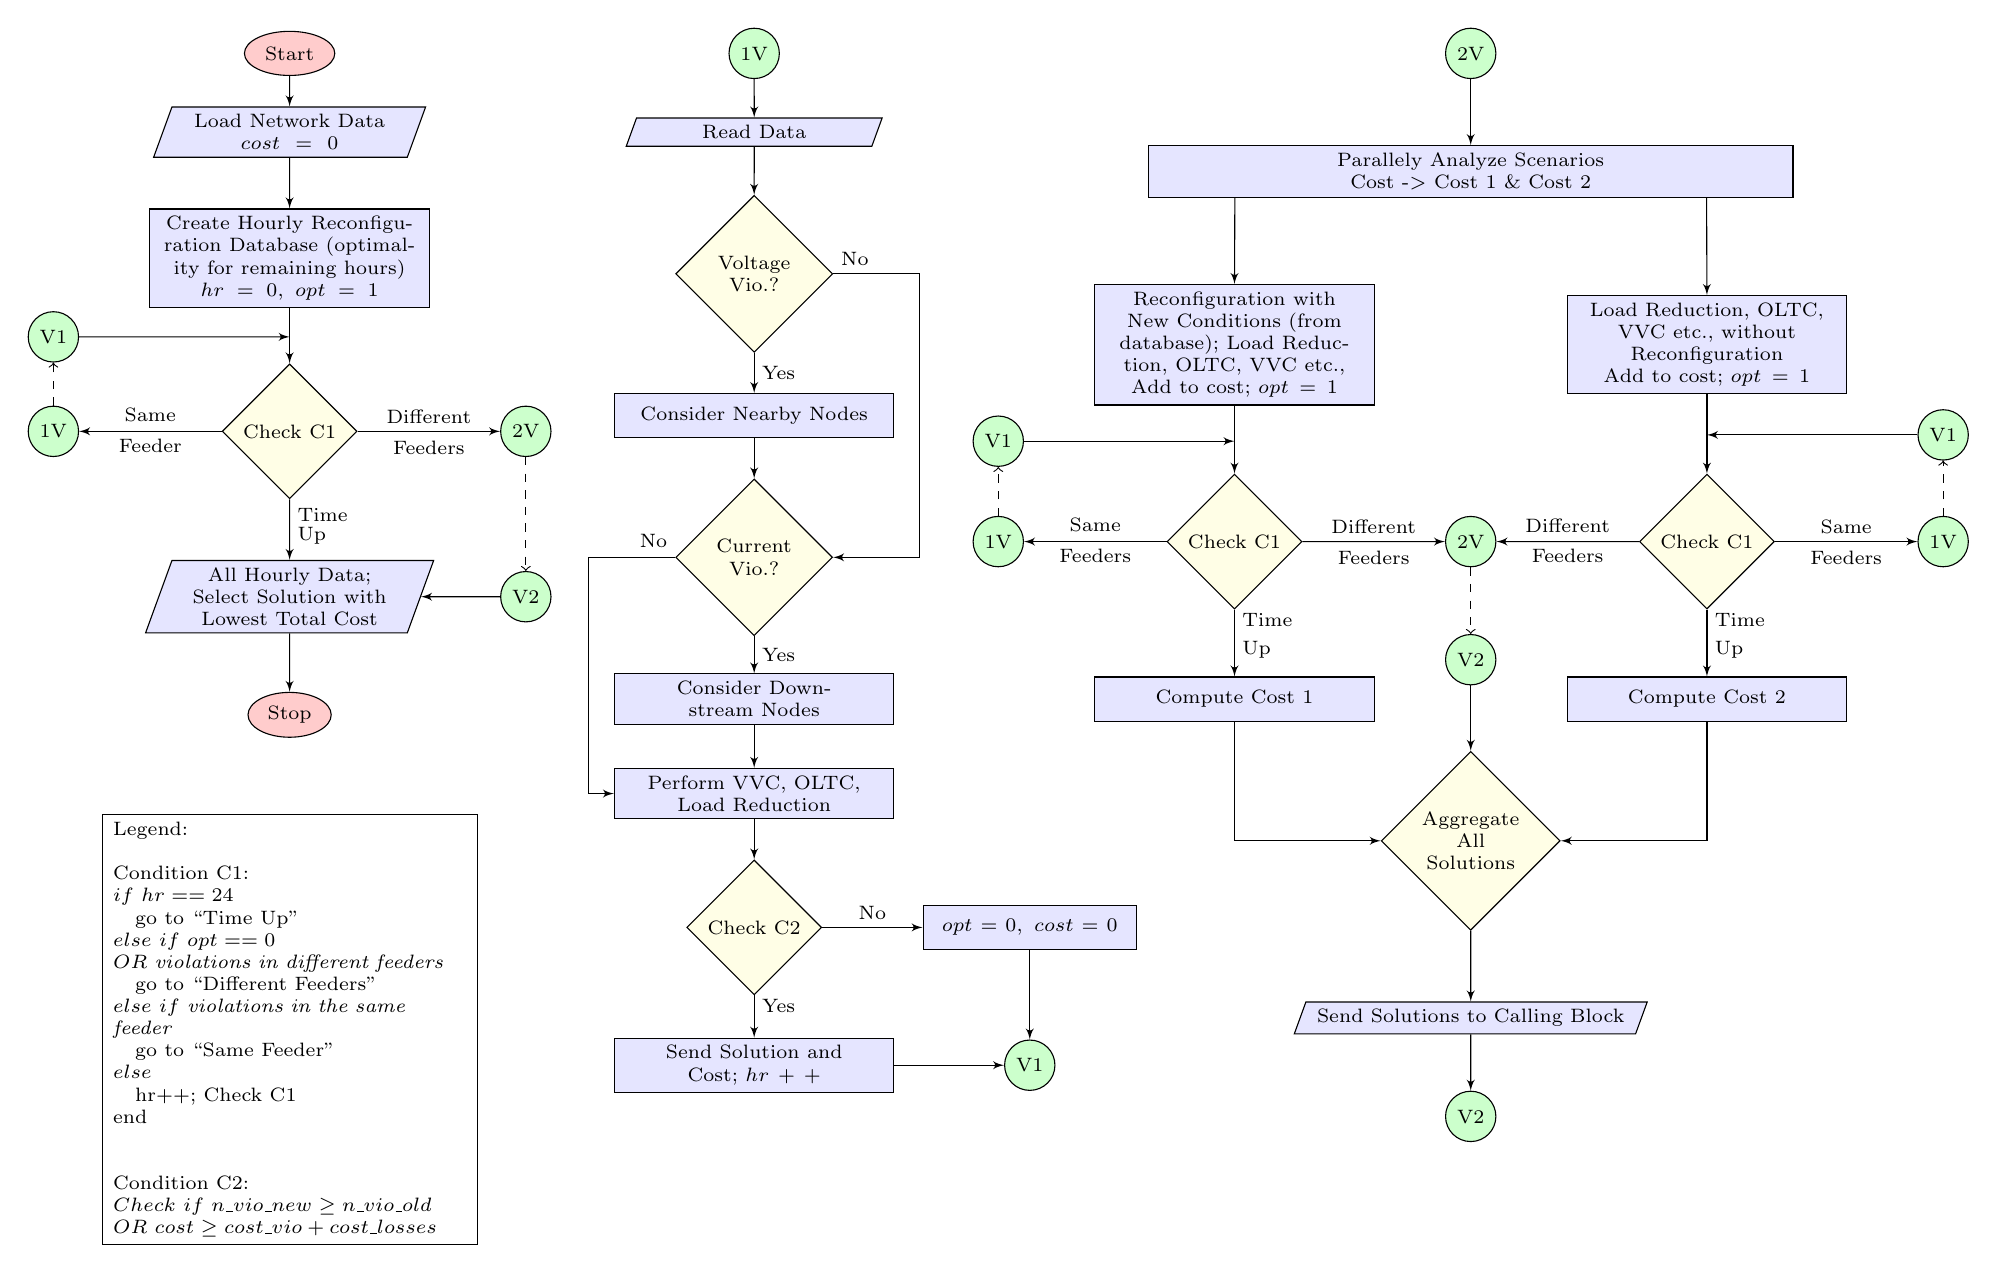
\begin{tikzpicture}[node distance = 1.5cm, auto]
\scriptsize

	% Define block styles
	\tikzstyle{decision} = [diamond, draw, fill=yellow!10, 
    text width=4.5em, text badly centered, node distance=3cm, inner sep=2pt]
	\tikzstyle{block} = [rectangle, draw, fill=blue!10, 
    text width=12em, text centered, minimum height=2em, minimum width=12em]
	\tikzstyle{io} = [trapezium, trapezium left angle=70, trapezium right angle=110, text centered, text width=10em, minimum width=10em, draw, fill=blue!10]
	\tikzstyle{line} = [draw, -latex']
	\tikzstyle{cloud} = [draw, ellipse,fill=red!20, node distance=3cm,
    minimum height=2em]
	\tikzstyle{con} = [draw, circle,fill=green!20, node distance=3cm,
    minimum height=2em]
	\tikzstyle{blank} = [node distance=1cm,minimum width=-1cm]
	\tikzstyle{legend} = [rectangle, draw,
    text width=16em, minimum height=2em, minimum width=17em]

	% Main Flow Chart
	\node [blank] (start) {};
	\node [cloud, below of=start, node distance=0cm] (init) {Start};
   	\node [io, below of=init, node distance=1cm] (load) {Load Network Data\\$cost=0$};
	\node [block, below of=load, node distance=1.6cm] (rec1) {Create Hourly Reconfiguration Database (optimality for remaining hours)\\ $hr=0,\ opt=1$};
	\node [decision, below of=rec1, node distance=2.2cm] (check1) {Check C1};
	\node [blank, below of=rec1,node distance=1.0cm] (b1) {};
	\node [con, left of=b1] (V1_1) {V1};
	\node [con, left of=check1] (1V_1) {1V};
	\node [con, right of=check1] (2V_1) {2V};
	\node [con, below of=2V_1, node distance=2.1cm] (V2_1) {V2};
	\node [blank, below of=check1] (b2) {};
	\node [io, below of=check1, node distance=2.1cm] (fin1) {All Hourly Data;\\Select Solution with Lowest Total Cost};
	\node [cloud, below of=fin1, node distance=1.5cm] (stop) {Stop};

	% Main Flowchart Paths
	\path [line] (init) -- (load);
	\path [line] (load) -- (rec1);
	\path [line] (rec1) -- (check1);
	\path [line] (V1_1) -- ($(b1.east)!0.5!(b1.west)$);
	\path [line] (check1.west) -- node [yshift=1.4em]  {Same} node {Feeder} (1V_1);
	\draw[dashed,->] (1V_1) -- (V1_1);
	\path [line] (check1.east) -- node {Different} node  [yshift=-1.4em] {Feeders} (2V_1);
	\path [line] (V2_1) -- (fin1);
	\draw[dashed,->] (2V_1) -- (V2_1);
	\path [line] (check1) -- node [near start] {Time} node [yshift=-0.3em] {Up} (fin1);
	\path [line] (fin1) -- (stop);

	% V1 Flowchart
	\node [con, right of= start, node distance=5.9cm](1V) {1V};
	\node [io, below of=1V, node distance=1cm] (read1V) {Read Data};
	\node [decision, below of=read1V, node distance=1.8cm](des1V_V) {Voltage Vio.?};
	\node [block, below of=des1V_V, node distance=1.8cm] (conV) {Consider Nearby Nodes};
	\node [decision, below of=conV, node distance=1.8cm](des1V_I) {Current Vio.?};
	\node [block, below of=des1V_I, node distance=1.8cm] (conI) {Consider Downstream Nodes};
	\node [block, below of=conI, node distance=1.2cm] (write1V) {Perform VVC, OLTC, Load Reduction};
	\node [decision, below of=write1V, node distance=1.7cm] (ok1V) {Check C2};
	\node [block, right of=ok1V, node distance=3.5cm, minimum width=9em, text width=9em] (no1V) {$opt=0,\ cost = 0$};
	\node [block, below of=ok1V, node distance=1.75cm] (res1V) {Send Solution and Cost; $hr++$};
	\node [con, right of=res1V, node distance=3.5cm] (V1) {V1};

	% V1 Flowchart Paths
	\path [line] (1V) -- (read1V);
	\path [line] (read1V) -- (des1V_V);
	\path [line] (des1V_V) -- node {Yes} (conV);
	\path [line] (des1V_V.east) --  node [near start] {No} +(1.1,0) |- (des1V_I.east);
	\path [line] (conV) -- (des1V_I);
	\path [line] (des1V_I) -- node {Yes} (conI);
	\path [line] (des1V_I.west) --  node [near start,yshift=1.4em] {No} +(-1.1,0) |- (write1V.west);
	\path [line] (conI) -- (write1V);
	\path [line] (write1V) -- (ok1V);
	\path [line] (ok1V) --  node [near start] {Yes} (res1V);
	\path [line] (ok1V) -- node {No} (no1V);
	\path [line] (no1V) -- (V1);
	\path [line] (res1V) -- (V1);

	% V2 Flowchart
	\centering
	\node [con, right of= start, node distance=15cm](2V) {2V};
	\node [block, below of=2V,minimum width=8cm,text width=8cm] (parallel) {Parallely Analyze Scenarios\\Cost -$>$ Cost 		1 \& Cost 2};
	\node [blank, below of=parallel, node distance=2.2cm] (bx) {};
	\node [block, left of=bx, node distance=3cm] (reconf) {Reconfiguration with New Conditions (from database); Load Reduction, OLTC, VVC etc.,\\ Add to cost; $opt=1$};
	\node [block, right of=bx, node distance=3cm] (lrvvc) {Load Reduction, OLTC, VVC etc., without Reconfiguration\\ Add to cost; $opt=1$};
	\node [blank, below of=reconf, node distance=1.225cm] (b3) {};
	\node [decision, below of=reconf, node distance=2.5cm] (check2) {Check C1};
	\node [con, left of=b3] (V1_2) {V1};
	\node [con, left of=check2] (1V_2) {1V};
	\node [block, below of=check2, node distance=2cm] (C1) {Compute Cost 1};

	\node [con, below of=2V, node distance=6.2cm] (2V_2) {2V};
	\node [con, below of=2V_2, node distance=1.5cm] (V2_2) {V2};
	\node [blank, below of=check2] (b4) {};
	\node [blank, below of=lrvvc, node distance=1.145cm] (b5) {};
	\node [decision, below of=lrvvc, node distance=2.5cm] (check3) {Check C1};
	\node [con, right of=b5] (V1_3) {V1};
	\node [con, right of=check3] (1V_3) {1V};
	\node [block, below of=check3, node distance=2cm] (C2) {Compute Cost 2};

	\node [decision, below of=parallel, node distance=8.5cm] (check4) {Aggregate All Solutions};
	\node [io, below of=check4, node distance=2.25cm, text width=4cm] (fin2) {Send Solutions to Calling Block};
	\node [con, below of=fin2, node distance=1.25cm] (V2) {V2};
	
	%V2 Flowchart Paths
	\path [line] (2V) -- (parallel);
	\path [line]  ($(parallel.south)!0.7305!(parallel.south west)$) -- (reconf.north);
	\path [line]  ($(parallel.south)!0.7305!(parallel.south east)$) -- (lrvvc.north);
	\path [line] (reconf) -- (check2);
	\path [line] (lrvvc) -- (check3);
	\path [line] (V1_2) -- ($(b3.east)!0.5!(b3.west)$);
	\path [line] (V1_3) -- ($(b5.east)!0.5!(b5.west)$);
	\path [line] (check2.east) -- node {Different} node  [yshift=-1.4em] {Feeders} (2V_2);
	\path [line] (check3.west) -- node  [yshift=1.4em] {Different} node {Feeders} (2V_2);
	\path [line] (V2_2) -- (check4);
	\draw[dashed,->] (2V_2) -- (V2_2);
	\path [line] (check2.west) -- node  [yshift=1.4em] {Same} node {Feeders} (1V_2);
	\path [line] (check3.east) -- node {Same} node  [yshift=-1.4em] {Feeders} (1V_3);
	\draw[dashed,->] (1V_2) -- (V1_2);
	\draw[dashed,->] (1V_3) -- (V1_3);
	\path [line] (check2) --  node [near start, yshift=0.3em] {Time} node [yshift=-0.3em] {Up} (C1);
	\path [line] (check3) --  node [near start, yshift=0.3em] {Time} node [yshift=-0.3em] {Up} (C2);
	\path [line] (C2.south) |- (check4.east);
	\path [line] (C1.south) |- (check4.west);
	\path [line] (check4.south) -- (fin2);
	\path [line] (fin2) -- (V2);

	% Legend
	\node [legend, below of=stop, node distance=4cm] (leg) {Legend:\\ \ \\Condition C1:\\$if\ hr == 24$\\\ \ \ go to ``Time Up''\\$else\ if\ opt == 0$\\$OR$ \textit{violations in different feeders}\\\ \ \ go to ``Different Feeders''\\$else\ if$ \textit{violations in the same feeder}\\\ \ \ go to ``Same Feeder''\\$else$\\\ \ \ hr++; Check C1\\end\\ \ \\ \ \\Condition C2:\\$Check\ if\ n\_vio\_new \ge n\_vio\_old$\\$OR\ cost \ge cost\_vio+cost\_losses$};

\end{tikzpicture}
\caption{The Flowchart of the Algorithm}
\labelFigure{fig:algoflch}
\end{sidewaysfigure}
%-------------------------------------------------------|
%-------------------------------------------------------|
%					 Flow Chart End 					|
%-------------------------------------------------------|
%-------------------------------------------------------|
\backmatter
\renewcommand{\bibname}{References}
% SVN info for this file
\svnidlong
{$HeadURL$}
{$LastChangedDate$}
{$LastChangedRevision$}
{$LastChangedBy$}

\RaggedRight
\nocite{*}
\printbibliography




\end{document}
